\chapter{Background}
\section{Hematology} % Taken from Sensors Survey DONE
Hematology is the branch of medicine concerned with the study, diagnosis, monitoring, treatment, and prevention of blood and blood-forming organs diseases. Hematology studies the blood in health and pathological conditions, firstly to identify the patient's health condition and, secondly, to predict how the bone marrow may have contributed to reaching that condition. 
Hematology, indeed, studies the relationship between the bone marrow and the systemic circulation. Many diseases, disorders, and deficiencies can affect the number and type of produced blood cells, their function, and lifespan. Usually, only healthy, mature or nearly mature cells are released into the bloodstream, but certain circumstances can induce the bone marrow to release immature and abnormal cells into the circulation. The Complete Blood Count (CBC) is one of the most frequently ordered tests to monitor the cell components distribution into the bloodstream. It offers various hematologic data represented by the numbers and types of cells in the peripheral blood circulation. The cells percentage is compared with the reference ranges to determine if the cells are present in their expected rate, if one cell type is increased, decreased or if immature cells exist. Reference ranges for blood tests are sets of values used to interpret a set of diagnostic test results from blood samples. Since it is difficult to prove that healthy-considered subjects may not have infections, parasitic infection and nutritional deficiency, it is more feasible to talk about reference ranges rather than normal ranges. A reference range is usually defined as the set of values in which 95\% of the healthy population falls within. It is determined by collecting data from vast numbers of laboratory tests result from a large number of subjects who are assumed to be representative of the population. With automatic counters or the flow cytometry, an automated CBC can be performed quickly. However, if the results from an automated cell count indicate the presence of abnormal cells or if there is a reason to suspect that abnormal cells are present, then a blood smear is collected \cite{Loddo2016}. A blood smear is often used to categorize and identify conditions that affect one or more types of blood cells and to monitor individuals undergoing treatment for these conditions. The results of a blood smear analysis typically include a description of the appearance of the cells, as well as any abnormalities that may be seen on the slide. The manual analysis of blood smears is tedious, lengthy, repetitive and it suffers from the presence of a non-standard precision because it depends on the operator's skill. The use of image processing techniques can help to analyze, count the cells in human blood and, at the same time, to provide useful and precise information about cells morphology.
Peripheral blood smears analysis is a common and economical diagnosis technique by which expert pathologists may obtain health information about the patients. Although this procedure requires highly trained experts, it is error-prone and could be affected by inter-observer variations. Moreover, blood cells' images taken from a microscope could vary in their illumination and coloration conditions, as shown in Figure \ref{fig:images_types}. Typically, blood cells images contain three main components of interest: the platelets (or thrombocytes), the red blood cells (or erythrocytes) and the white blood cells (or leukocytes). It is worth considering that blood cells exist with different shapes, characteristics, and colorations, according to their types. A schematic representation is shown in Fig. \ref{fig:leukocytes2}
Many tests are designed to determine the number of erythrocytes and leukocytes in the blood, together with the volume, sedimentation rate, and hemoglobin concentration of the red blood cells (blood count). Besides, certain tests are used to classify blood according to specific red blood cell antigens, or blood groups. Other tests elucidate the shape and structural details of blood cells and hemoglobin and other blood proteins. Blood can be analyzed to determine the activity of various enzymes or protein catalysts, that either is associated with the blood cells or are found free in the blood plasma.
Blood also may be analyzed from properties such as total volume, circulation time, viscosity, clotting time and clotting abnormalities, acidity (pH), levels of oxygen and carbon dioxide, and the clearance rate of various substances. There are specific tests based on the presence in the blood of substances characteristic of specific infections, such as the serological tests for syphilis, hepatitis, and human immunodeficiency virus (HIV, the AIDS virus) \cite{Brit}.
Among the several available blood tests, the most common are the blood cells counts, \mbox{e.g., a CBC} is a measure of the hematologic parameters of the blood. Included in the CBC is the calculation of the number of red blood cells (red blood cell count) or white blood cells (white blood cell count) in a cubic millimeter (mm$^{3}$) of blood, a differential white blood cell count, a hemoglobin assay, a hematocrit, calculations of red cell volume, and a platelet count. The differential white blood cell count includes measurements of the different types of white blood cells that constitute the total white blood cell count: the band neutrophils, segmented neutrophils, lymphocytes, monocytes, eosinophils, and basophils. A specific infection can be suspected from the type of leukocyte that has an abnormal value \cite{DiRuberto2016}.

\begin{figure}[h]
	\centering
	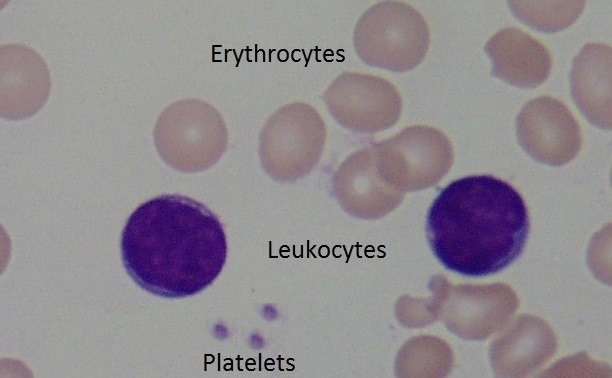
\includegraphics[width=0.3\textwidth]{images/Cells1}
	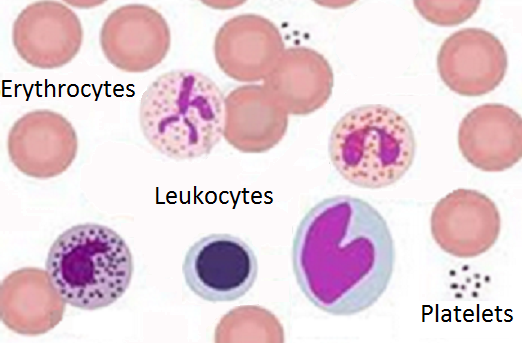
\includegraphics[width=0.3\textwidth]{images/Cells2}
	\caption[Peripheral blood smear components.]{\label{fig:leukocytes2} Peripheral blood smear components: a real image and a schematic representation.}
\end{figure}

\begin{figure}[h]
	\centering    
	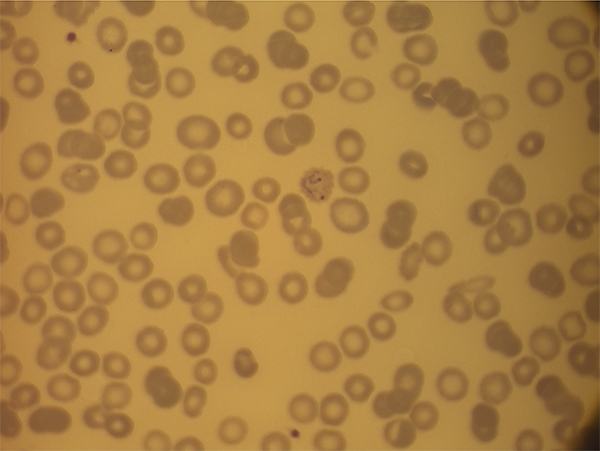
\includegraphics[width=0.22\textwidth]{images/malaria/f1a}
	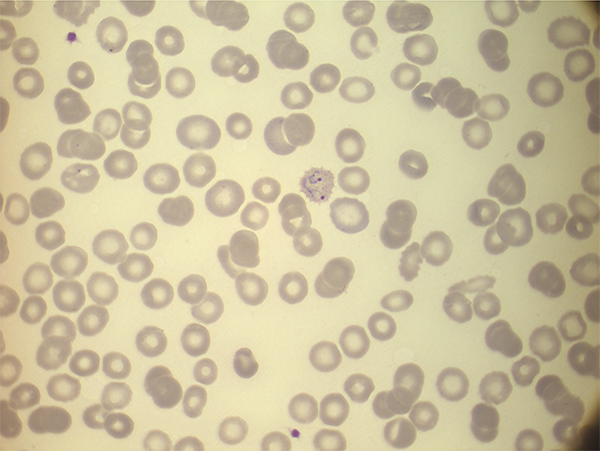
\includegraphics[width=0.22\textwidth]{images/malaria/f1b}
	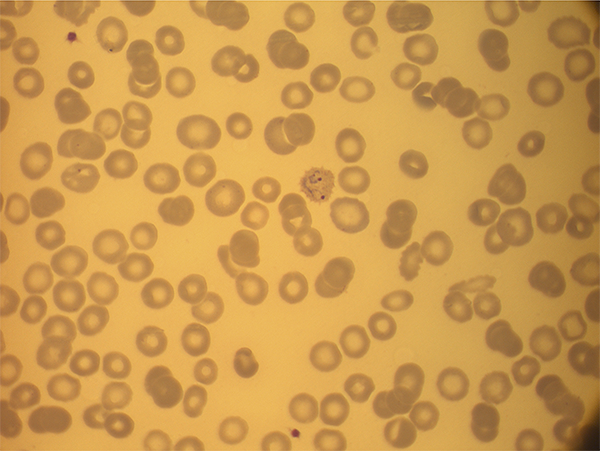
\includegraphics[width=0.22\textwidth]{images/malaria/f1c}
	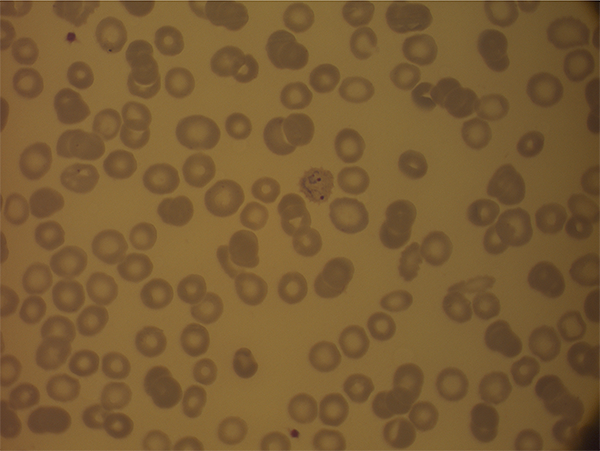
\includegraphics[width=0.22\textwidth]{images/malaria/f1d}
	\caption[Example of different illumination conditions.]{\label{fig:images_types} Different illumination conditions generate distinct images because of the absence of a standardized acquisition procedure. From left to right: acquisition of the same smear with four microscope's brightness levels. Courtesy of CHUV, Lausanne.}
\end{figure}

\section{Peripheral Blood Images}
There are several components in blood smears containing peripheral blood samples. Consequently, these kinds of image usually consist of, at least, three principal objects of interest: the White Blood Cells (\acs{WBC}s), the Red Blood Cells (\acs{RBC}s) and the platelets (or thrombocytes). 
Platelets or thrombocytes are small non-nucleated disc-shaped cells with a diameter between 1 and 3 $\mu$m. Upon release into the peripheral blood from the bone marrow, they appear as fragments. They play a significant role in hemostasis leading to the formation of blood clots when there is blood vessel injury or bleeding, starting to clump together to form aggregates. There must be a sufficient number of platelets to control bleeding. If too few are present, or if they do not work correctly, the ability to form a clot becomes impaired and can be a life-threatening situation \cite{Ciesla}. Healthy, mature RBCs or erythrocytes are uniform in size, 7-8 $\mu$m in diameter,  and do not have a nucleus as most other cells do. They are round and flattened like a donut with a depression in the middle instead of a hole (biconcave). Due to the hemoglobin inside the RBCs, they appear pink to red with a pale center once the staining process has been completed. Considering that not every RBC could respect its typical shape, any significant number of cells that are different in shape or size may indicate the presence of some diseases \cite{Erhabor}. WBCs or leukocytes have a nucleus surrounded by cytoplasm, instead. For this reason, they are easily identifiable, as their nucleus appears darker than the background. However, the analysis and the processing of data related to the WBCs are complicated due to wide variations in cell shape, dimensions, and edges. The generic term leukocyte refers to a set of cells that are entirely different from each other. Indeed, although they are all derived from bone marrow stem cells, in the bone marrow, they differentiate themselves into two main groups: cells containing granules, called granulocytic or myelocytic, and cells without granules called mononuclear or lymphoid. Thus, we can distinguish between these cells according to their shape or size, the presence of granules in the cytoplasm and the number of lobes in the nucleus, as it can be seen in Fig.~\ref{fig:leukocytes1}. The lobes are the most substantial part of the nucleus, and thin filaments connect them. WBCs mature into five distinct cells types, that include neutrophils, basophils, and eosinophils in the granulocytic group and lymphocytes and monocytes in the non-granulocytic group. Neutrophils are indeed the most common WBCs in a healthy adult, present in the human blood at a percentage ranging between 50 and 70\%. They range in size from 10-15 $\mu$m and present a cytoplasm with pink or purple granules. They are distinguishable also due to the number of lobes present in the nucleus, which can range from 1 to 6 according to the cell maturation. They are involved in the defense against infections.
Basophils are the least common of the granulocytes and represent only 0-1\% of all leukocytes in human blood. They have a diameter of approximately 10 $\mu$m. Generally, basophils have an irregular, plurilobated nucleus that is obscured by large and dark granules. Eosinophils are easily recognized in stained smears due to the presence of large, red-orange granules, which include para-crystalline structures in the shape of a coffee bean. They are round, 10-12 $\mu$m in size, and have a nucleus with two lobes. Generally low in number, present at 1-5\% in human blood, they most often increase in number in individuals with allergies and parasitic infections. Monocytes are usually the most voluminous WBCs, with a diameter of 12-20 $\mu$m and are often referred to as scavenger cells (phagocytes). They can ingest particles such as cellular debris, bacteria, or other insoluble particles. They represent 3-9\% of circulating leukocytes. Their nucleus is large and curved, often in the shape of a kidney. Lymphocytes are usually the smaller WBCs, with a diameter of 7-12 $\mu$m. They are characterized as having a smooth, round nucleus and a small amount of cytoplasm and often a smooth chromatin pattern. They are very common in human blood, with a percentage of 20-45\%. 

\begin{figure}[!htbp]
	\centering
	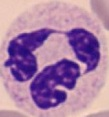
\includegraphics[height=0.125\textheight]{images/crop-Fig2-1}
	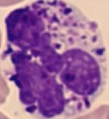
\includegraphics[height=0.125\textheight]{images/crop-Fig2-2}
	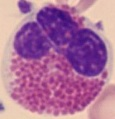
\includegraphics[height=0.125\textheight]{images/crop-Fig2-3}
	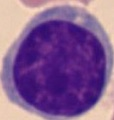
\includegraphics[height=0.125\textheight]{images/crop-Fig2-4}
	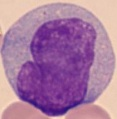
\includegraphics[height=0.125\textheight]{images/crop-Fig2-5}
	\caption[WBCs types comparison.]{\label{fig:leukocytes1}A comparison between different types of WBCs: neutrophils, basophils, eosinophils, monocytes and lymphocytes.}
\end{figure}

Numerous diseases and conditions can affect the absolute or relative number of WBCs and their appearance on a blood smear. More details of the conditions that affect the number and the morphology of kind of cells are listed in Appendix A. Examples of the most common diseases that involve variation in shape and number of blood cells include anemia, hemophilia, general blood clots, and bleeding disorders while more severe cases that need to be diagnosed are leukemia, myeloma, and lymphoma. This thesis focused on the analysis of Acute Lymphoblastic Leukemia (ALL) and malaria.

\section{ALL - Acute Lymphoblastic Leukemia}
Leukemia is a blood cancer that can be detected through the analysis of WBCs. There are two types of leukemia: acute and chronic. According to the French-American-British (FAB) classification model \cite{Bennett}, acute leukemia is classified into two subtypes: acute lymphoblastic leukemia (\acs{ALL}) and acute myeloid leukemia (AML). Here, only ALL has been considered, which affects a group of leukocytes called lymphocytes. ALL primarily affects children and adults over 50 years of age. The risk of developing ALL is highest in children younger than five years of age, and it declines and begins to rise again after age 50. Due to its rapid expansion into the bloodstream and vital organs, ALL can be fatal if left untreated \cite{Biondi}. Therefore, early diagnosis of this disease is crucial for a patients' recovery, especially for children. Diagnosis of ALL is based on the morphological identification of lymphocytes suffering from ALL, called lymphoblasts, by microscopy and the immunophenotypic assessment of lineage commitment and developmental stage \cite{Inaba}. Lymphoblasts present morphological changes that increment with increasing severity of the disease. In particular, lymphocytes are regularly shaped and have a compact nucleus with regular and continuous edges, whereas lymphoblasts are irregularly shaped and contain small cavities in the cytoplasm, termed vacuoles, and spherical particles within the nucleus, termed nucleoli \cite{Donida} (Fig.~\ref{fig:ex2}).

\begin{figure}[!t]
	\centering
	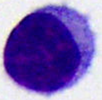
\includegraphics[height=0.125\textheight]{images/crop-BlastNo}
	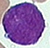
\includegraphics[height=0.125\textheight]{images/crop-BlastL1}
	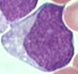
\includegraphics[height=0.125\textheight]{images/crop-BlastL2}
	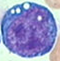
\includegraphics[height=0.125\textheight]{images/crop-BlastL3}
	\caption[Lymphocytes suffering from ALL comparison.]{\label{fig:ex2}A comparison between lymphocytes suffering from ALL: a healthy lymphocyte, followed by lymphoblasts classified as L1, L2 and L3, respectively, according to the FAB \cite{Bennett}.}
\end{figure}

The observation of blood smears by skilled operators is one diagnostic procedure available to initially recognize the ALL, where the automatic counter fails due to the presence of abnormal cells. Human visual inspection is tedious, lengthy and repetitive, and it suffers from the presence of a non-standard precision because it depends on the operator's skill; these disadvantages limit its statistical reliability. The use of image processing techniques can help count the cells in human blood and at the same time to provide information about cell morphology, making them less expensive and providing more accurate standards. One of the goals of this thesis is to provide a fully automatic procedure based on the analysis of blood smear images, to support medical activity. This procedure counts the WBCs present in the smear through a process of segmentation and detection. The detected WBCs are then classified as suffering from ALL or not. 

\subsection {Related Works}
The progress of automated methods for the classification of blood cells from digitized images is a current problem in pattern recognition. These techniques can help to count the cells in human blood and, at the same time, be able to provide information on the morphological cells themselves. Unfortunately, for the analysis and processing of images, there are no standard techniques to apply to all types of images, but the processing must be adapted to the context. In particular, regarding the blood smear images, the processing techniques vary according to the type of blood cell to be analyzed. In the literature, few attempts of automated systems, based on techniques of image processing, able to identify and classify peripheral blood cells have been proposed.
Moreover, the existing systems are only partially automated, combining manual steps to automated ones. Furthermore, most of them do not work on the entire analysis process, but on individual phases of the whole analysis process. This section will show the techniques most commonly used by different authors at different stages of the process. 

The used methods of pre-processing depend on many variables, such as lighting conditions, the duration of the dye, defects caused by visual artifacts or not uniform background. The images should be processed to improve specific characteristics or to reduce further operations that could be required in the later stages of the analysis. The main issues addressed at this stage include noise reduction and enhancement of some structures of the images. Mohapatra et al. \cite{Mohapatra10a, Mohapatra10b, Mohapatra10c, Mohapatra14} used a median filter to remove the noise followed by an Unsharp filter. The median filter has been preferred to the average filter since it preserves details of edges and then they are enhanced with the use of the Unsharp filter. Other authors preferred operations based on the histogram such as contrast stretching or the histogram equalization to redistribute the grey level values. Often these two transformations have been used together or with other techniques, as the algorithm proposed in \cite{Madhloom}. It starts from the greyscale image performs separately a contrast stretching and a histogram equalization. Then a series of arithmetic operations between the two images just obtained is performed in order to highlight the nuclei of leukocytes. The results are impressive because it either enhances the nuclei of leukocytes and it drastically reduces the number of the other blood components, making further steps much more straightforward.

As previously said, different levels of segmentation are used in medical images analysis. In particular, for what concerns peripheral blood images two main levels are used: the level of cells segmentation, which aims to separate whole cells from the background or plasma and the level of segmentation that tries to separate the various components inside the cell, such as the nucleus from the cytoplasm or intracellular parasites. Several authors have proposed methods for effective segmentation of the nucleus of leukocytes, while there are few attempts of segmentation of the cytoplasm. The characteristic generally used for segmentation is the intensity value of grey level images. However, many authors showed how the use of a single channel from different color spaces could be used to highlight differences between blood components. Indeed the nuclei of the white blood cells are more in contrast on the Green component of the RGB color space \cite{Cseke}, while the cytoplasm of the white blood cells is more evident on the Hue component \cite{Wu} or the Saturation component \cite{Halim} of the HSV color space. The Saturation component of the HSV color space is also useful to identify and separate erythrocytes \cite{DiR} when present in complex agglomerates of cells. Otherwise, they can be easily detected and counted with a threshold value computed using Zack algorithm from grey level images \cite{Berge}. Based on this knowledge many algorithms of region growing have been proposed \cite{Kovalev, Lez98, Lez02}. They use the pixels within the nuclei as seeds in order to segment the whole white blood cells. The cytoplasm is detected through iterative aggregation of the pixels surrounding the region of interest according to the homogeneity of the colors and the information of the gradient. Edge-based segmentation methods are rarely used in this contest since the boundaries between cells are not clearly defined. However, the performances of edge detection operations can be improved using morphological operators \cite{Piuri, Sco05} being able to connect in a better way the detected edges and restore the complete boundary of the cells. 
A huge number of papers has been proposed in the literature concerning the application
of clustering methods to the segmentation of medical images \cite{Karthikeyan2017}

A further problem in the analysis of peripheral blood cell images is the presence of cells grouped together or adjacent, as shown in Fig. \ref{fig_clumps}. It does not allow an analysis of the single cells, such as the computation of shape descriptors or the proportion of cytoplasm and nucleus. A priori knowledge about the average size and shape of the cells allow working on sub-images extracted from the original image, by cutting a square around the nucleus previously segmented \cite{Kovalev, Sinha}. Thus, assuming that each sub-image has only one white blood cell using some restrictions on the shape and the color information it is possible to perform a clustering around the nucleus. Unfortunately, this assumption is not always true, and in fact, it is possible to find more than one nucleus on a sub-image that affects the result of the clustering. An improvement of this approach works on the whole images without using the a priori knowledge about the size and shape. It is possible thanks to the distance transform \cite{Maurer} that associates to each pixel of the binary image its distance from the border. Thus, the maximum distance obtained can be used as a marker for a subsequent segmentation step \cite{Malpica}, or the distance image can be used directly as a shape delimiter for a watershed segmentation \cite{Lindblad}. The main drawbacks of these approaches are that the cells should be perfectly segmented since they work directly on the binary images. Furthermore, since the distance transform, in this case, works like a shape delimiter, it can separate only small agglomerates of cells that should have an almost circular shape.

Finally, \cite{Chen2016} proposed a deep learning method for cells classification in a label-free environment. They also compared various learning algorithms including artificial neural network, support vector machine, logistic regression.

\begin{figure}[h]
	\centering
	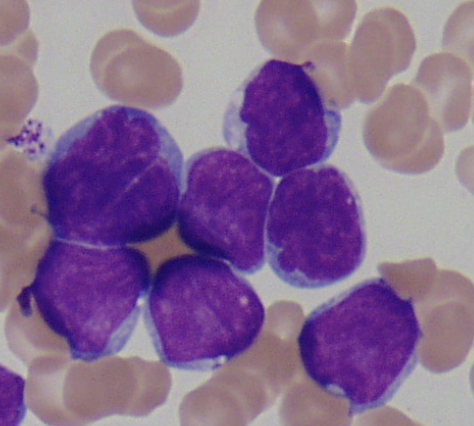
\includegraphics[height=0.25\textwidth]{images/2016_1_mva/clump}
	\caption[ALL-IDB1 image crop.]{\label{fig_clumps}Crop of a sample image taken from ALL-IDB1. It represents a leukocyte clump.}
\end{figure}

The step of feature extraction is essential in the analysis of peripheral blood cells, as only with significant features, the system will be able to discriminate the various types of cells, the cells affected by diseases from the normal ones or the presence of other abnormalities in the blood. The idea is to extract the descriptors that best approach to the visual patterns indicated by pathologists. The color and texture descriptors are indeed the most discriminatory features of blood cells. Generally, this kind of images is acquired using the RGB color space that allows good discrimination of platelets, red blood cells, and white blood cells, especially if the analysis is extended to all RGB channels \cite{Angulo}. However, the differentiation of subclasses of cells such as various types of leukocytes, usually requires the use of other color spaces, taking into account all the color channels or only the most discriminatory such as the H channel of the HSV color space \cite{Hengen}.
Furthermore, geometrical features can be used to discriminate cells with abnormal size or with an irregular shape. Other geometrical features have explicitly been proposed to classify the type of nucleated cells since they can be distinguished not only using the ratio between cytoplasm and nucleus \cite{Piuri, Sco05, Sco06} but also extracting the number of lobes of the nucleus. Extract the number of lobes means to count the more substantial parts of the nucleus connected by thin filaments. It is not an easy task since the connection between the lobes sometimes can appear larger than average and thus, also a skilled operator, could count two small lobes as it was only one. A good approximation of the number of lobes can be obtained by iterative erosion of the nucleus. The number of lobes corresponds to the connected components with an area more significant than a prefixed parameter \cite{Piuri}.  

Once the features have been extracted, they must be inserted in a process which classifies cells based on hematological concepts \cite{Biondi, Serbouti}. 
Different learning methods have been used to classify blood cells, but above all very different choices about the number of classes have been taken. The most frequent choice is the binary classification to distinguish healthy white blood cells from abnormal ones making use of the SVM classifier, which is excellent in the separation of binary classes with a pattern very close in space \cite{Mohapatra10a, Mohapatra10b, Mohapatra10c, Mohapatra14}. Mishra \cite{Mishra2017} showed that a highly appropriate feature extraction technique is required for the classification of the disease. Discrete Cosine Transform (DCT) has been used in association with a nucleus features extraction from the RGB image. Finally, they detect ALL on ALL-IDB images with SVM classifier.
KNN classifier is also used, for example Abdeldaim et al. \cite{Abdeldaim2018} present a computer-aided ALL diagnosis system, which first segments each cell in the microscopic images, and then classifies each segmented cell to be normal or affected. The experiment based on ALL-IDB2 achieves the
accuracy of 96.42\% with a KNN classifier. Instead, when the number of classes is higher the most used classifier have been the Neural Networks, performing a separation into the five types of leukocytes \cite{Sco06} or performing a separation into 7 classes, lymphocytes, neutrophils, eosinophils, other (monocytes and basophils), lymphocytic leukaemia L1, lymphocytic leukaemia L2 and non-lymphocytic leukaemia \cite{Buavirat}. 

In the following chapter, you will see the algorithms proposed to create a fully automated system for peripheral blood images. For clarity, each step of the whole process has been discussed separately following the order mentioned before and used for most of the methods presented in the literature. Furthermore, to make a comparison with the state-of-the-art, each step of the proposed method has been tested using the same dataset presented below.

\subsection{White Blood Cells images Datasets}
\label{wbc_datasets}
The main problem in the testing phase of an automated system is certainly the absence of many public datasets. A lot of authors have tested their methods by using only manual segmented ground truth samples or private datasets. These disadvantages do not allow a direct comparison with the results obtained by similar proposed systems, and it limits the reproducibility of possible innovations. Among the public datasets of peripheral blood samples image we found useful for our purposes, there are the following:
\begin{itemize}
	\item ALL-IDB \cite{Donida}
	\item IUMS-IDB \cite{Sarrafzadeh}
	\item SMC-IDB \cite{Mohamed}
\end{itemize} 
Acute Lymphoblastic Leukemia Image Database (\acs{ALL-IDB}), has been proposed by Donida Labati in \cite{Donida}. It is a public image dataset of peripheral blood samples of normal individuals and leukemic patients, and it contains the relative supervised classification and segmentation data. So, this dataset allows not only to assess the quality of the algorithms for cell counting but also to assess the ability to discriminate the white blood cells affected by leukemia from healthy ones. The sample images have been collected by the experts of the M. Tettamanti Research Center for childhood leukemia and hematological diseases, Monza, Italy. The ALL-IDB database has two distinct versions. The first version the ALL-IDB1 contains full-size original images that can be used for testing the segmentation capability of algorithms, as well as the classification systems and image preprocessing methods. The second version the ALL-IDB2 is a collection of cropped area of interest of normal and blast cells that belong to the ALL-IDB1 dataset, so it can be used only for testing the performances of classification systems.

\begin{figure}[!htbp]
	\centering
	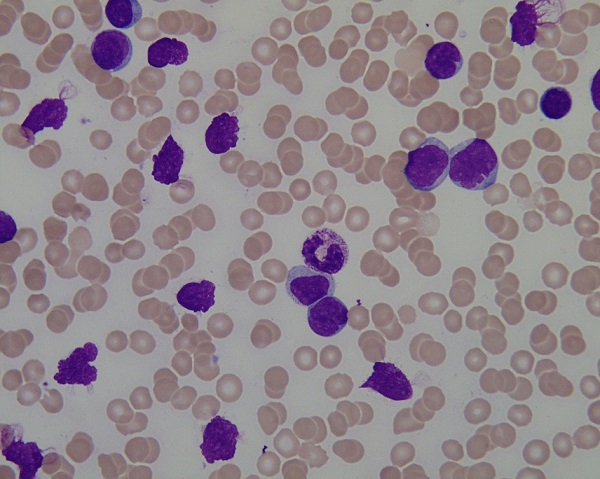
\includegraphics[height=0.25\textwidth]{images/Fig17-1}
	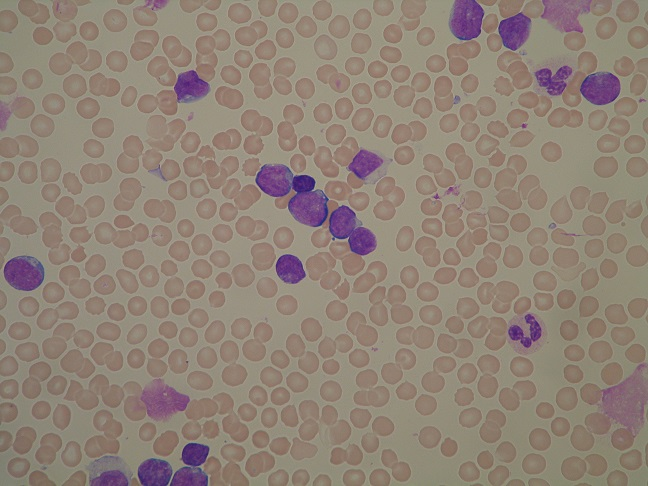
\includegraphics[height=0.25\textwidth]{images/Fig17-2}
	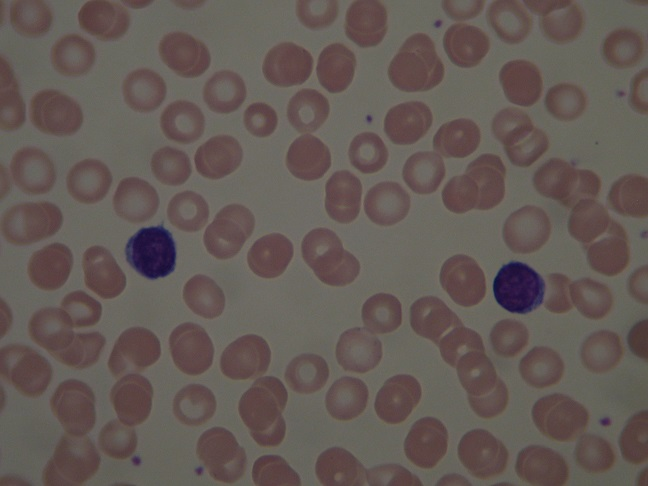
\includegraphics[height=0.25\textwidth]{images/Fig17-3}
	\caption[ALL-IDB1 samples.]{\label{fig:dataset}Sample images from the ALL-IDB1}
\end{figure}

In both versions of the dataset, each image has an associated text file containing the coordinates of the centroid of each candidate lymphoblast, which was manually labeled by a skilled operator and can be used as ground truth for classification. The dataset ALL-IDB1 includes 108 images in JPG format with 24-bit color depth. Most of the images in the dataset were captured with an optical laboratory microscope, with different magnifications ranging from 300 to 500, coupled with a Canon PowerShot G5 camera and their resolution is 2592x1944. The remaining images were acquired with a microscope at a constant magnification, combined with an Olympus C2500L camera and their resolution is 1712x1368. Some images belonging to the ALL-IDB1 are shown in Fig.~\ref{fig:dataset}.

\begin{figure}[!htbp]
	\centering
	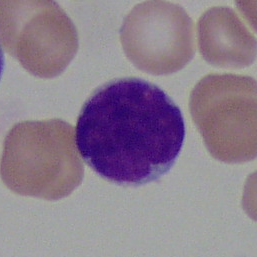
\includegraphics[height=0.16\textwidth]{images/Fig18-1}
	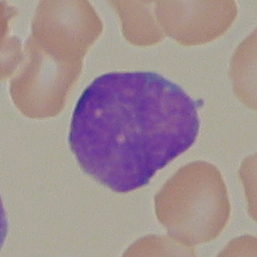
\includegraphics[height=0.16\textwidth]{images/Fig18-2}
	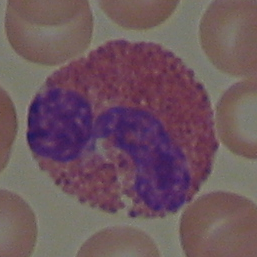
\includegraphics[height=0.16\textwidth]{images/Fig18-3}
	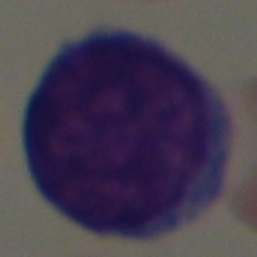
\includegraphics[height=0.16\textwidth]{images/Fig18-4}
	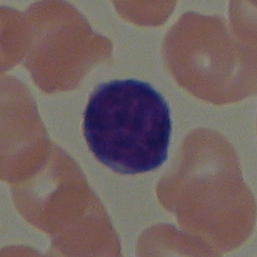
\includegraphics[height=0.16\textwidth]{images/Fig18-5}
	\caption[ALL-IDB2 samples.]{\label{fig:dataset2}Sample images from the ALL-IDB2}
\end{figure}

The sample images show that there are many differences either regarding color and illumination or resolution and cells dimension. The dataset ALL-IDB2 includes 260 images in TIFF format with 24-bit color depth. As said previously, these images are cropped areas of interest, containing a single leukocyte per image, belonging from the first version of the database. These images, differently from the first ones, have a standard size of $257\times257$, but being cropped area of them, they present the same issues about color, illumination and cells dimension, as it can be seen in Fig.~\ref{fig:dataset2}.

\begin{figure}[ht]
	\centering
	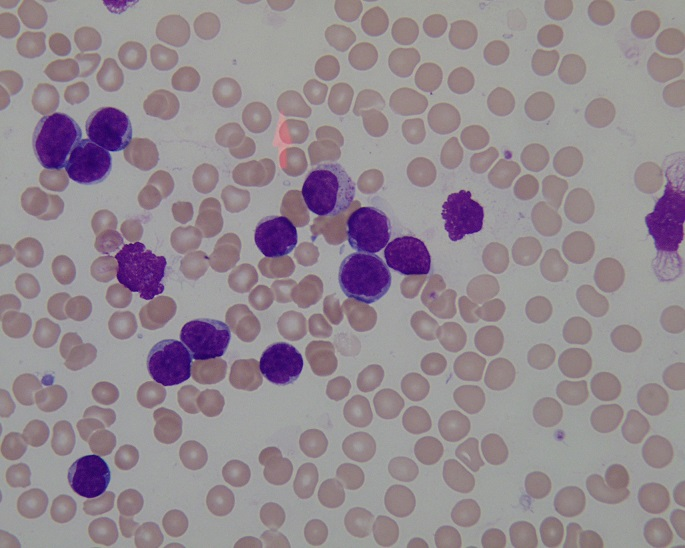
\includegraphics[width=0.24\textwidth]{images/Im003_1}\vspace{1 mm}
	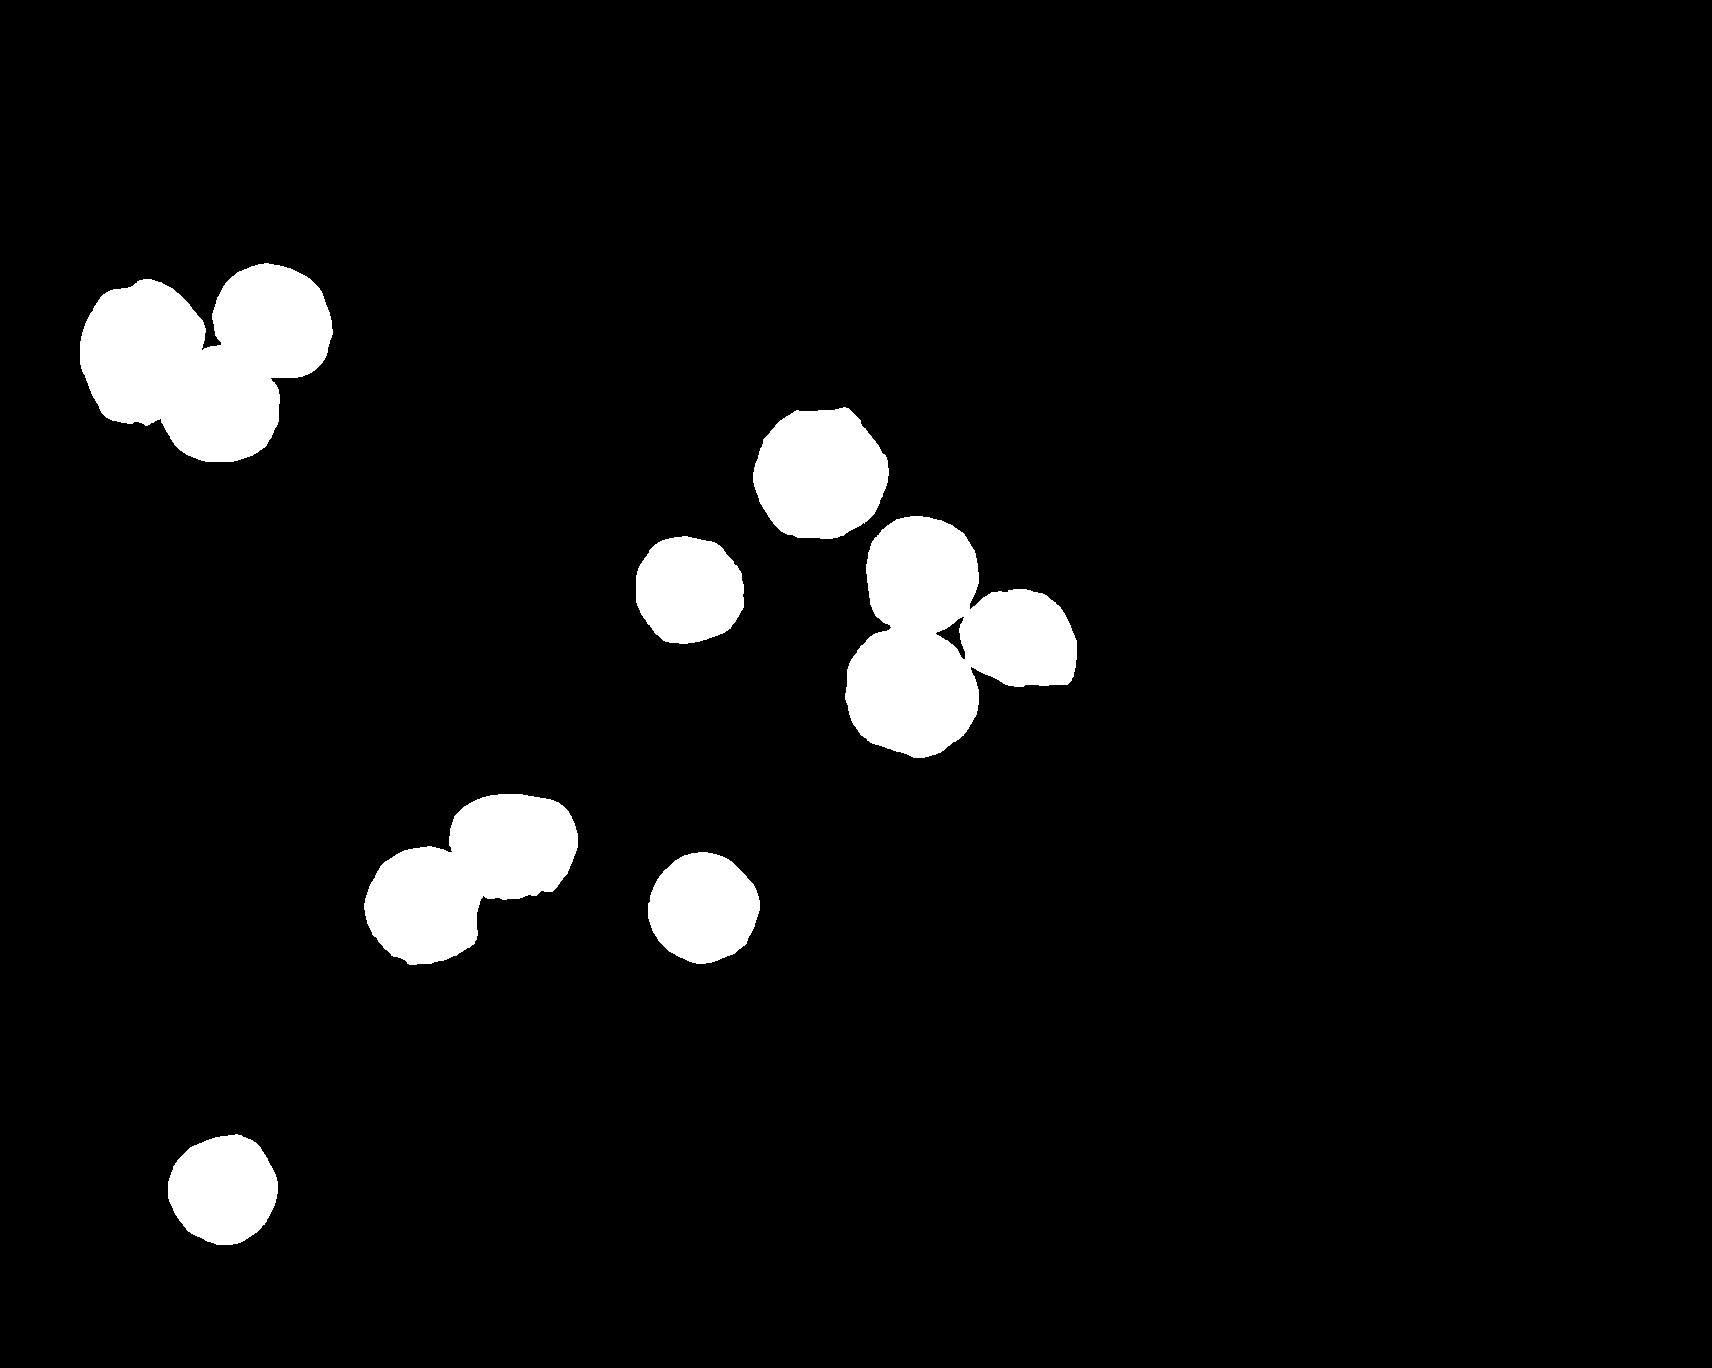
\includegraphics[width=0.24\textwidth]{images/Im003_1_WBC}
	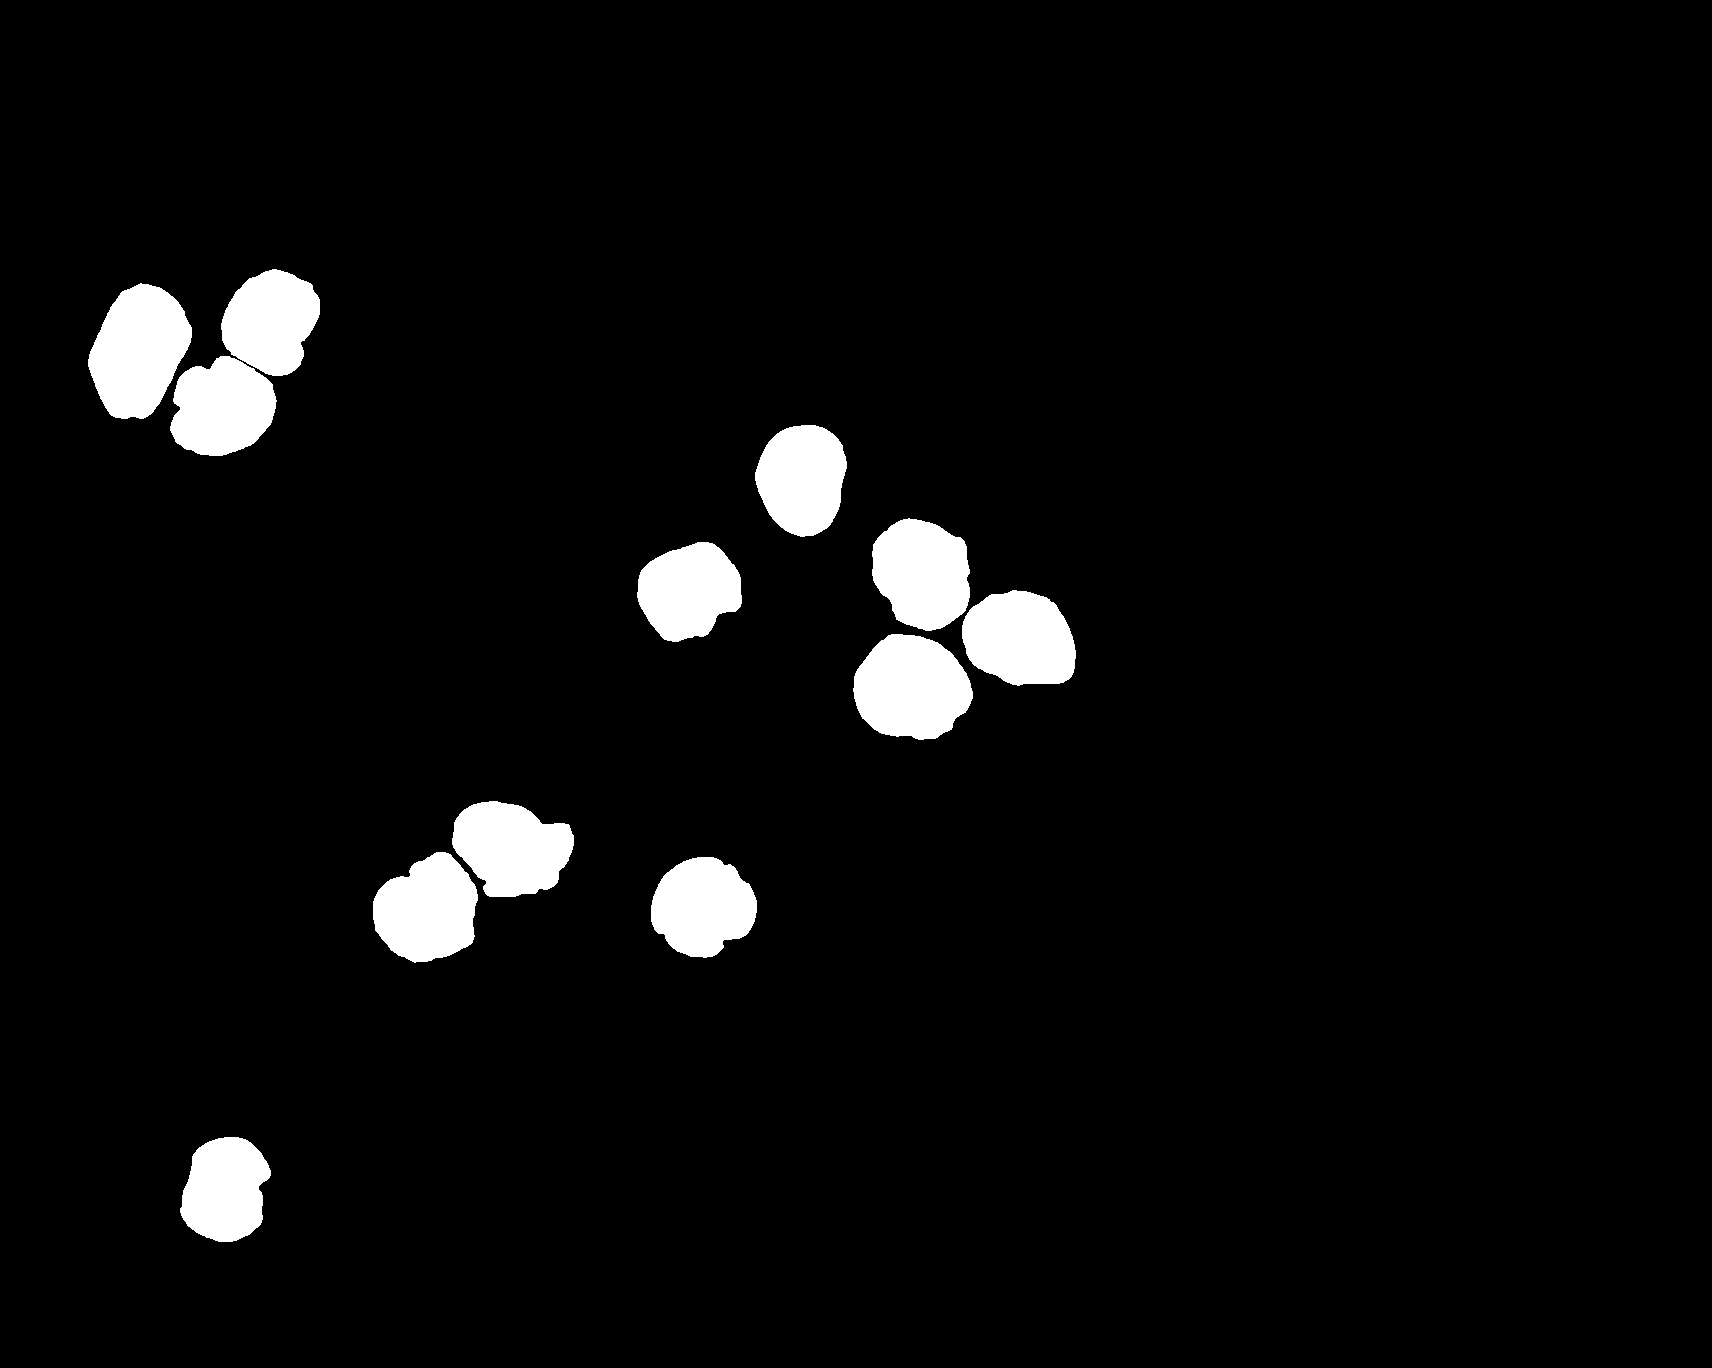
\includegraphics[width=0.24\textwidth]{images/Im003_1_WBCn}
	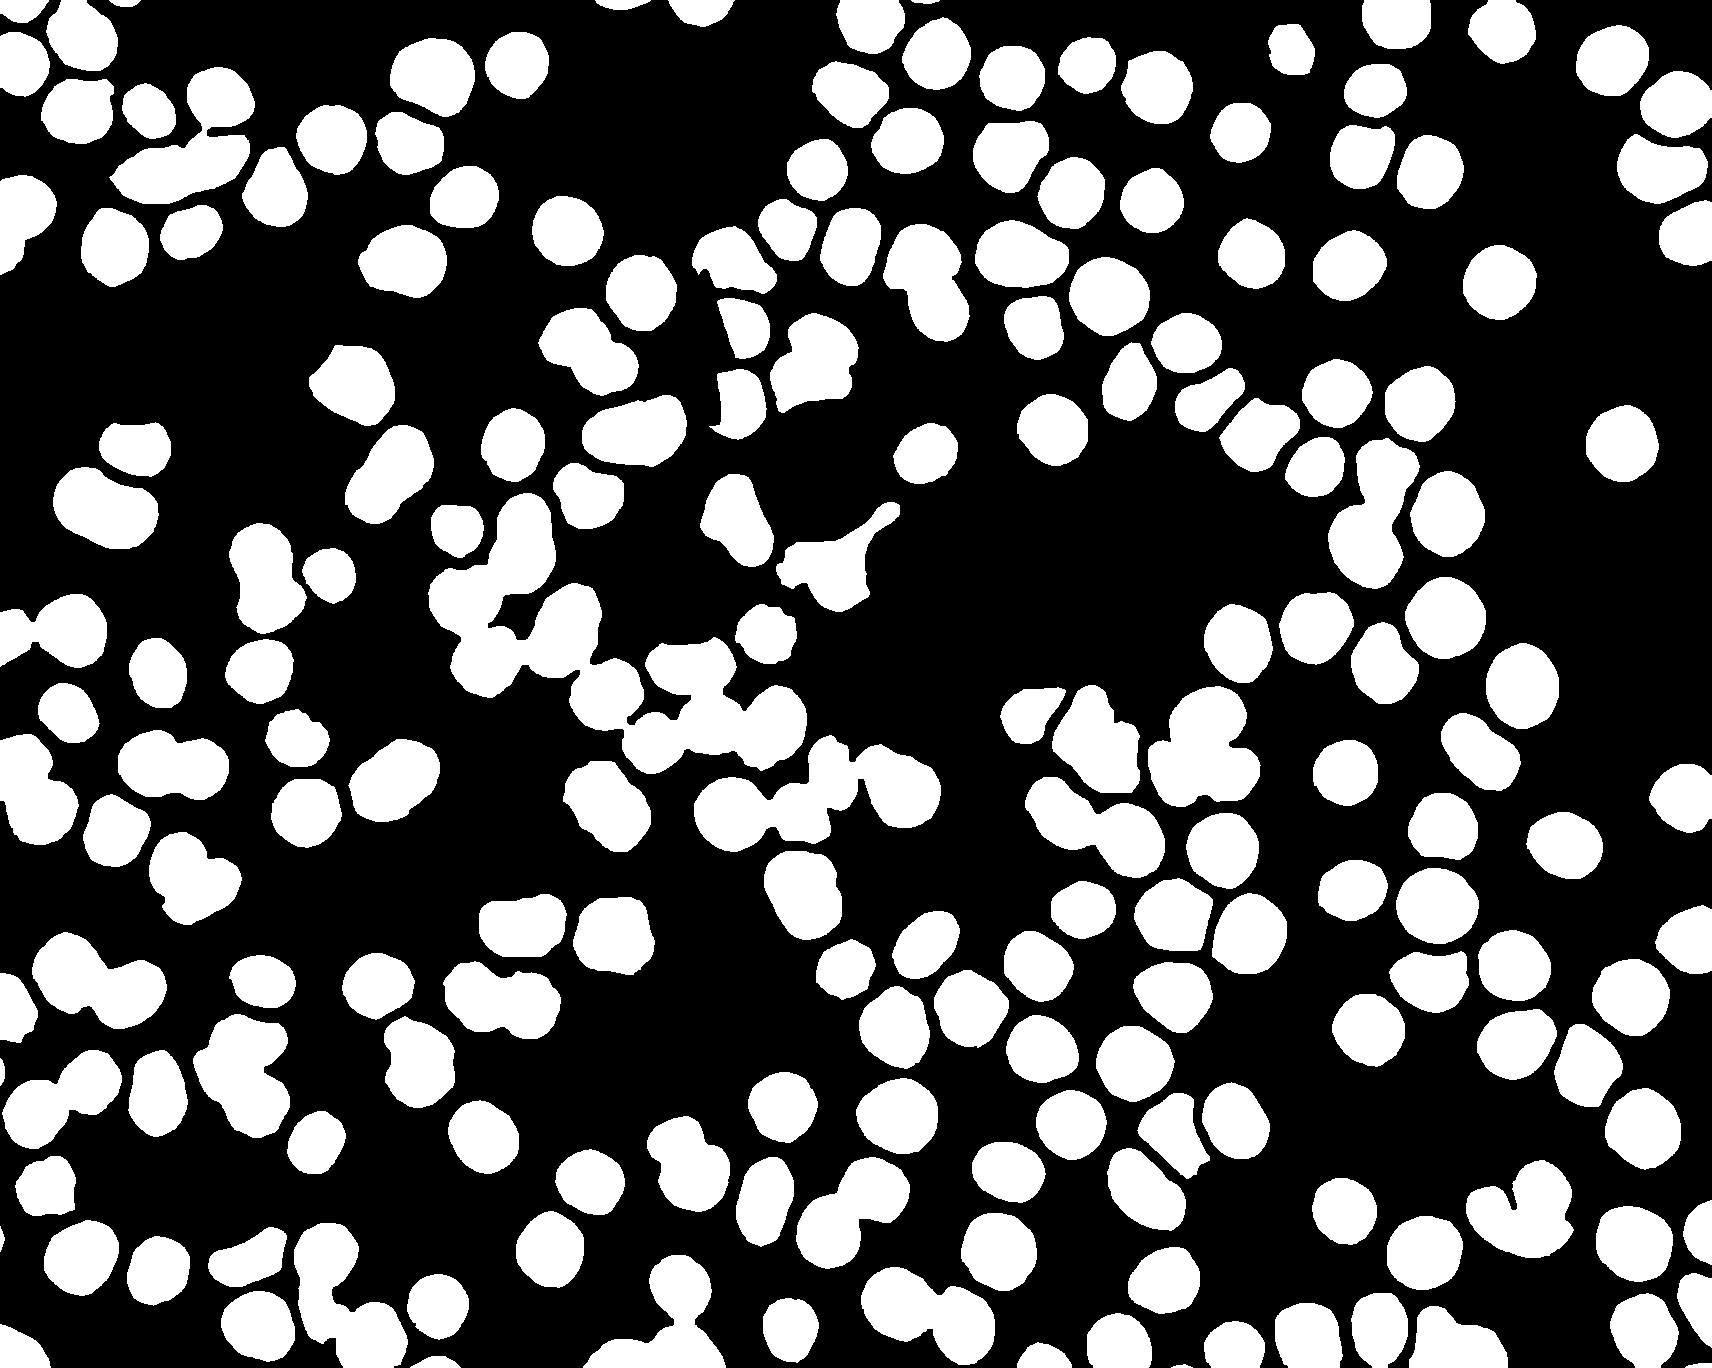
\includegraphics[width=0.24\textwidth]{images/Im003_1_RBC}
	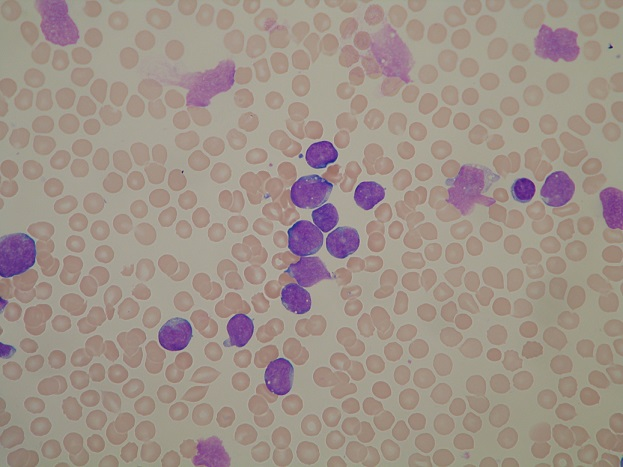
\includegraphics[width=0.24\textwidth]{images/Im050_1}
	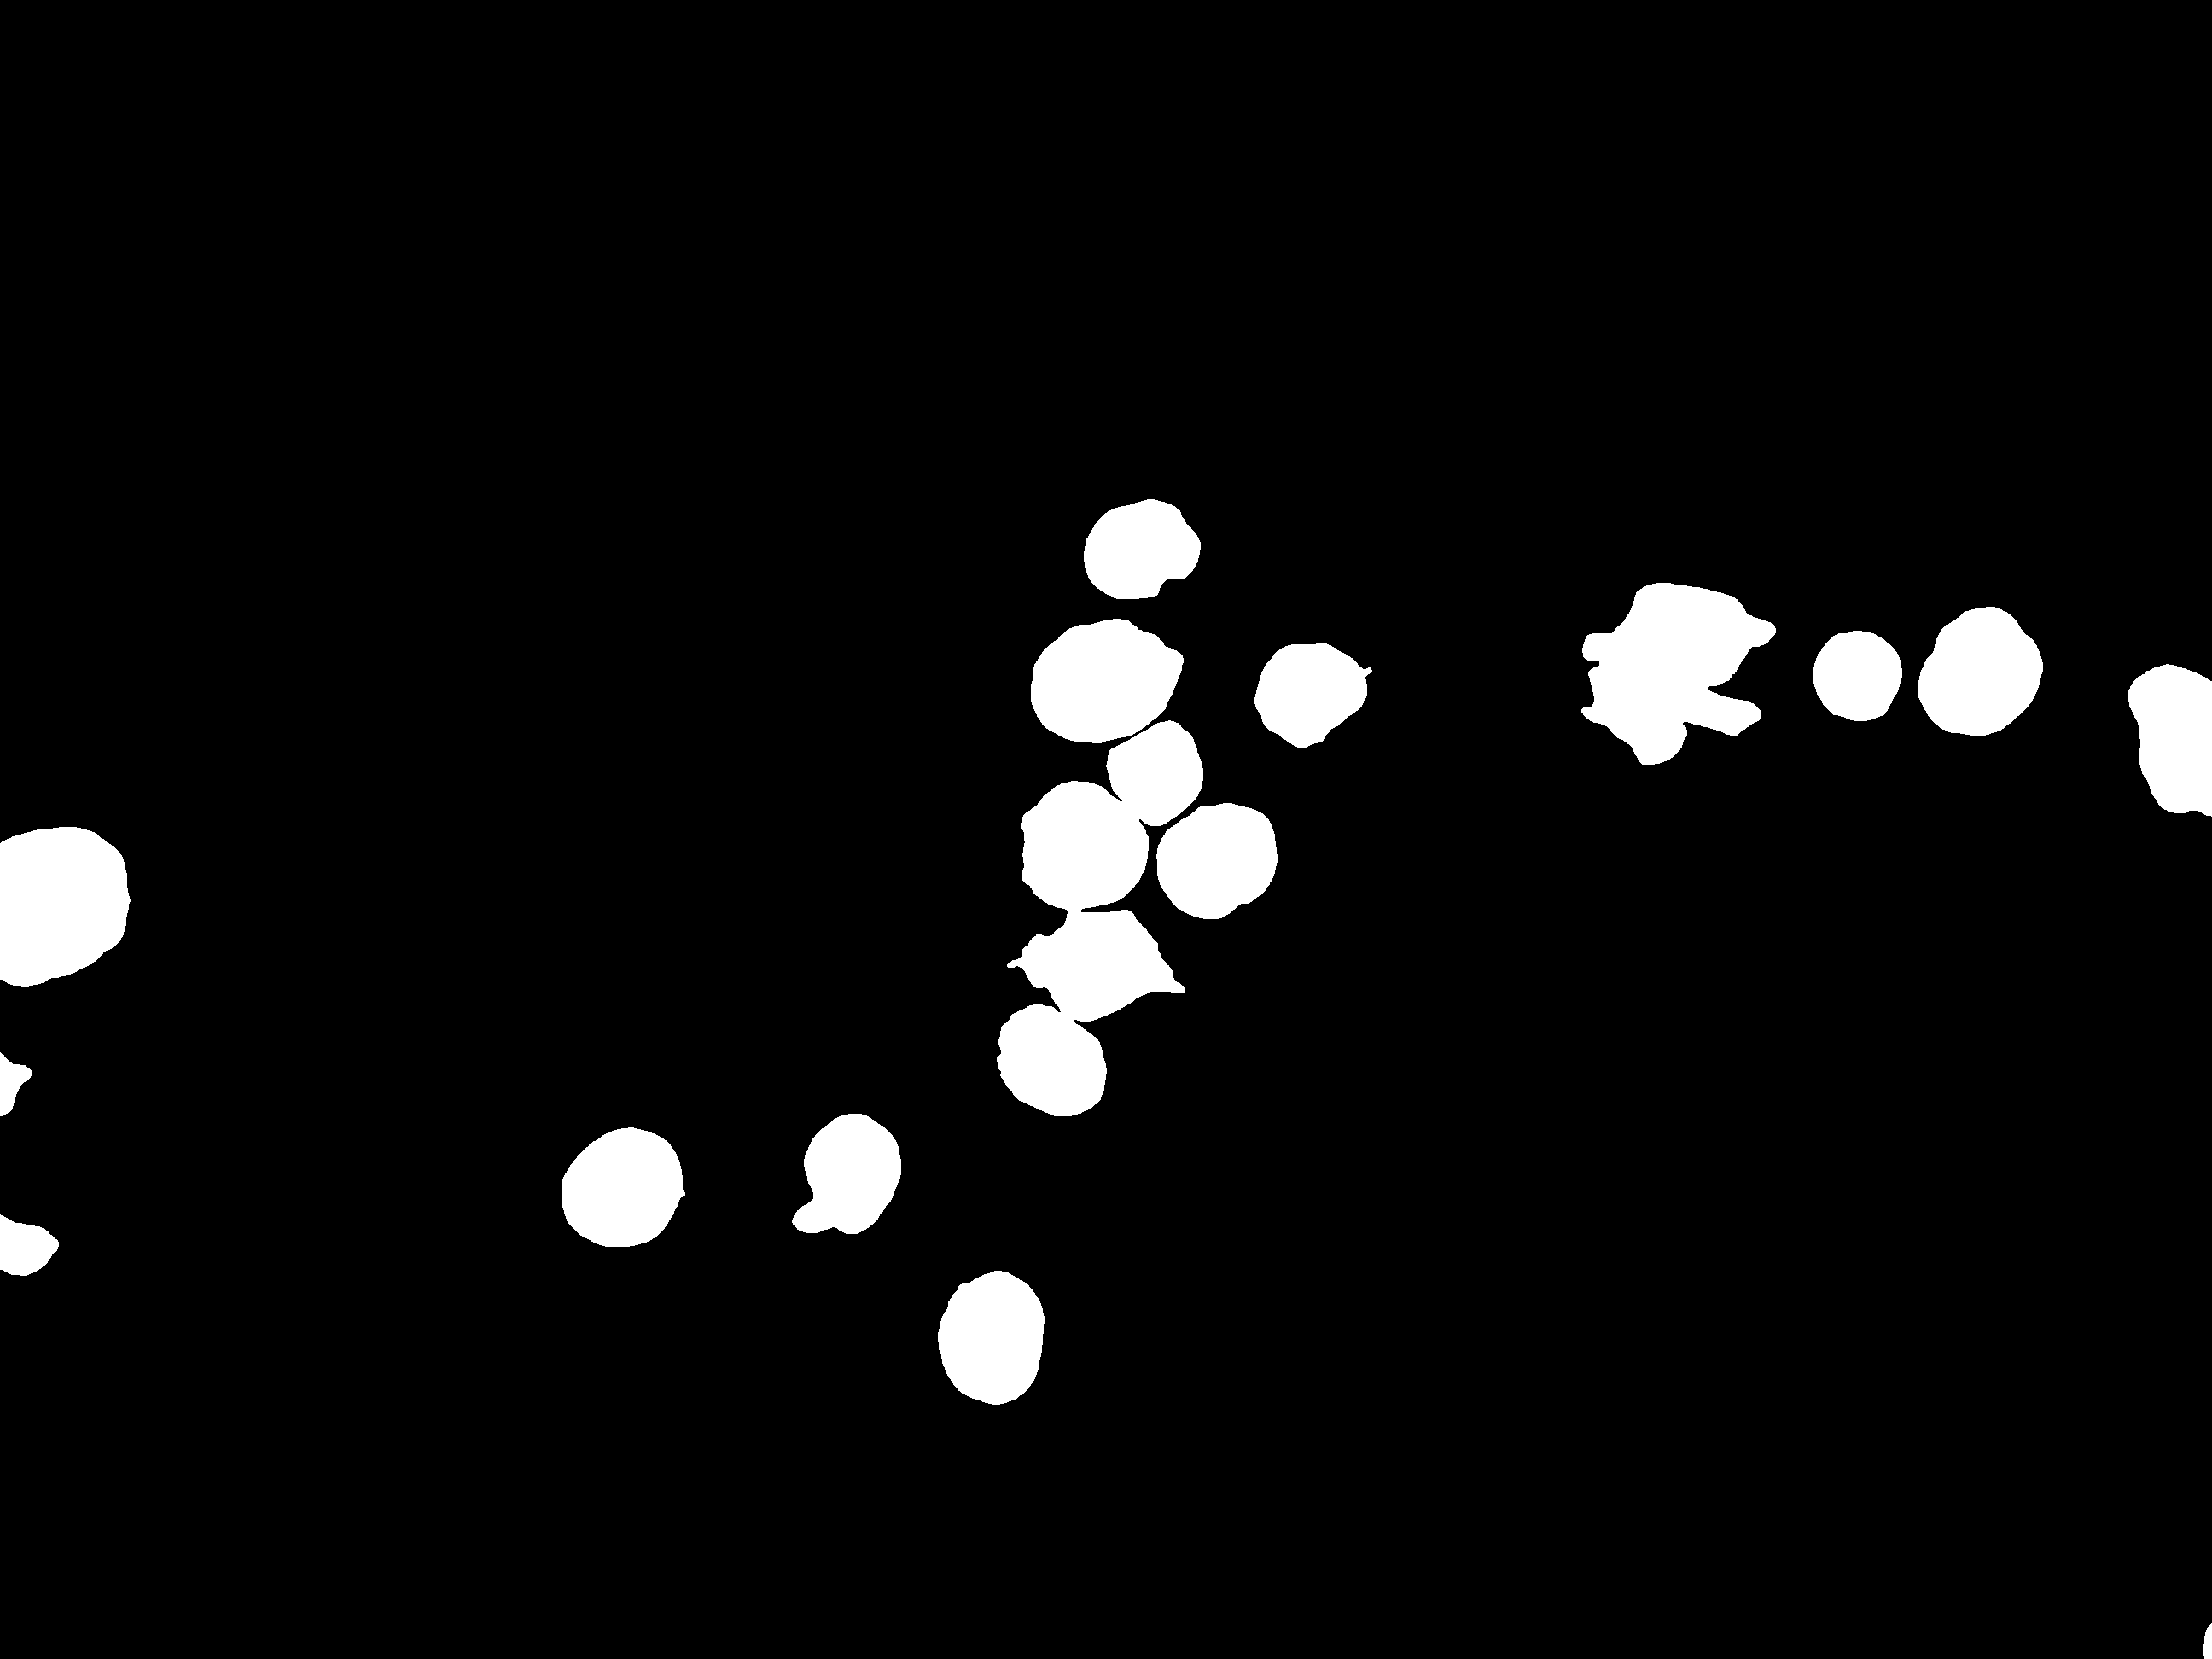
\includegraphics[width=0.24\textwidth]{images/Im050_1_WBC}
	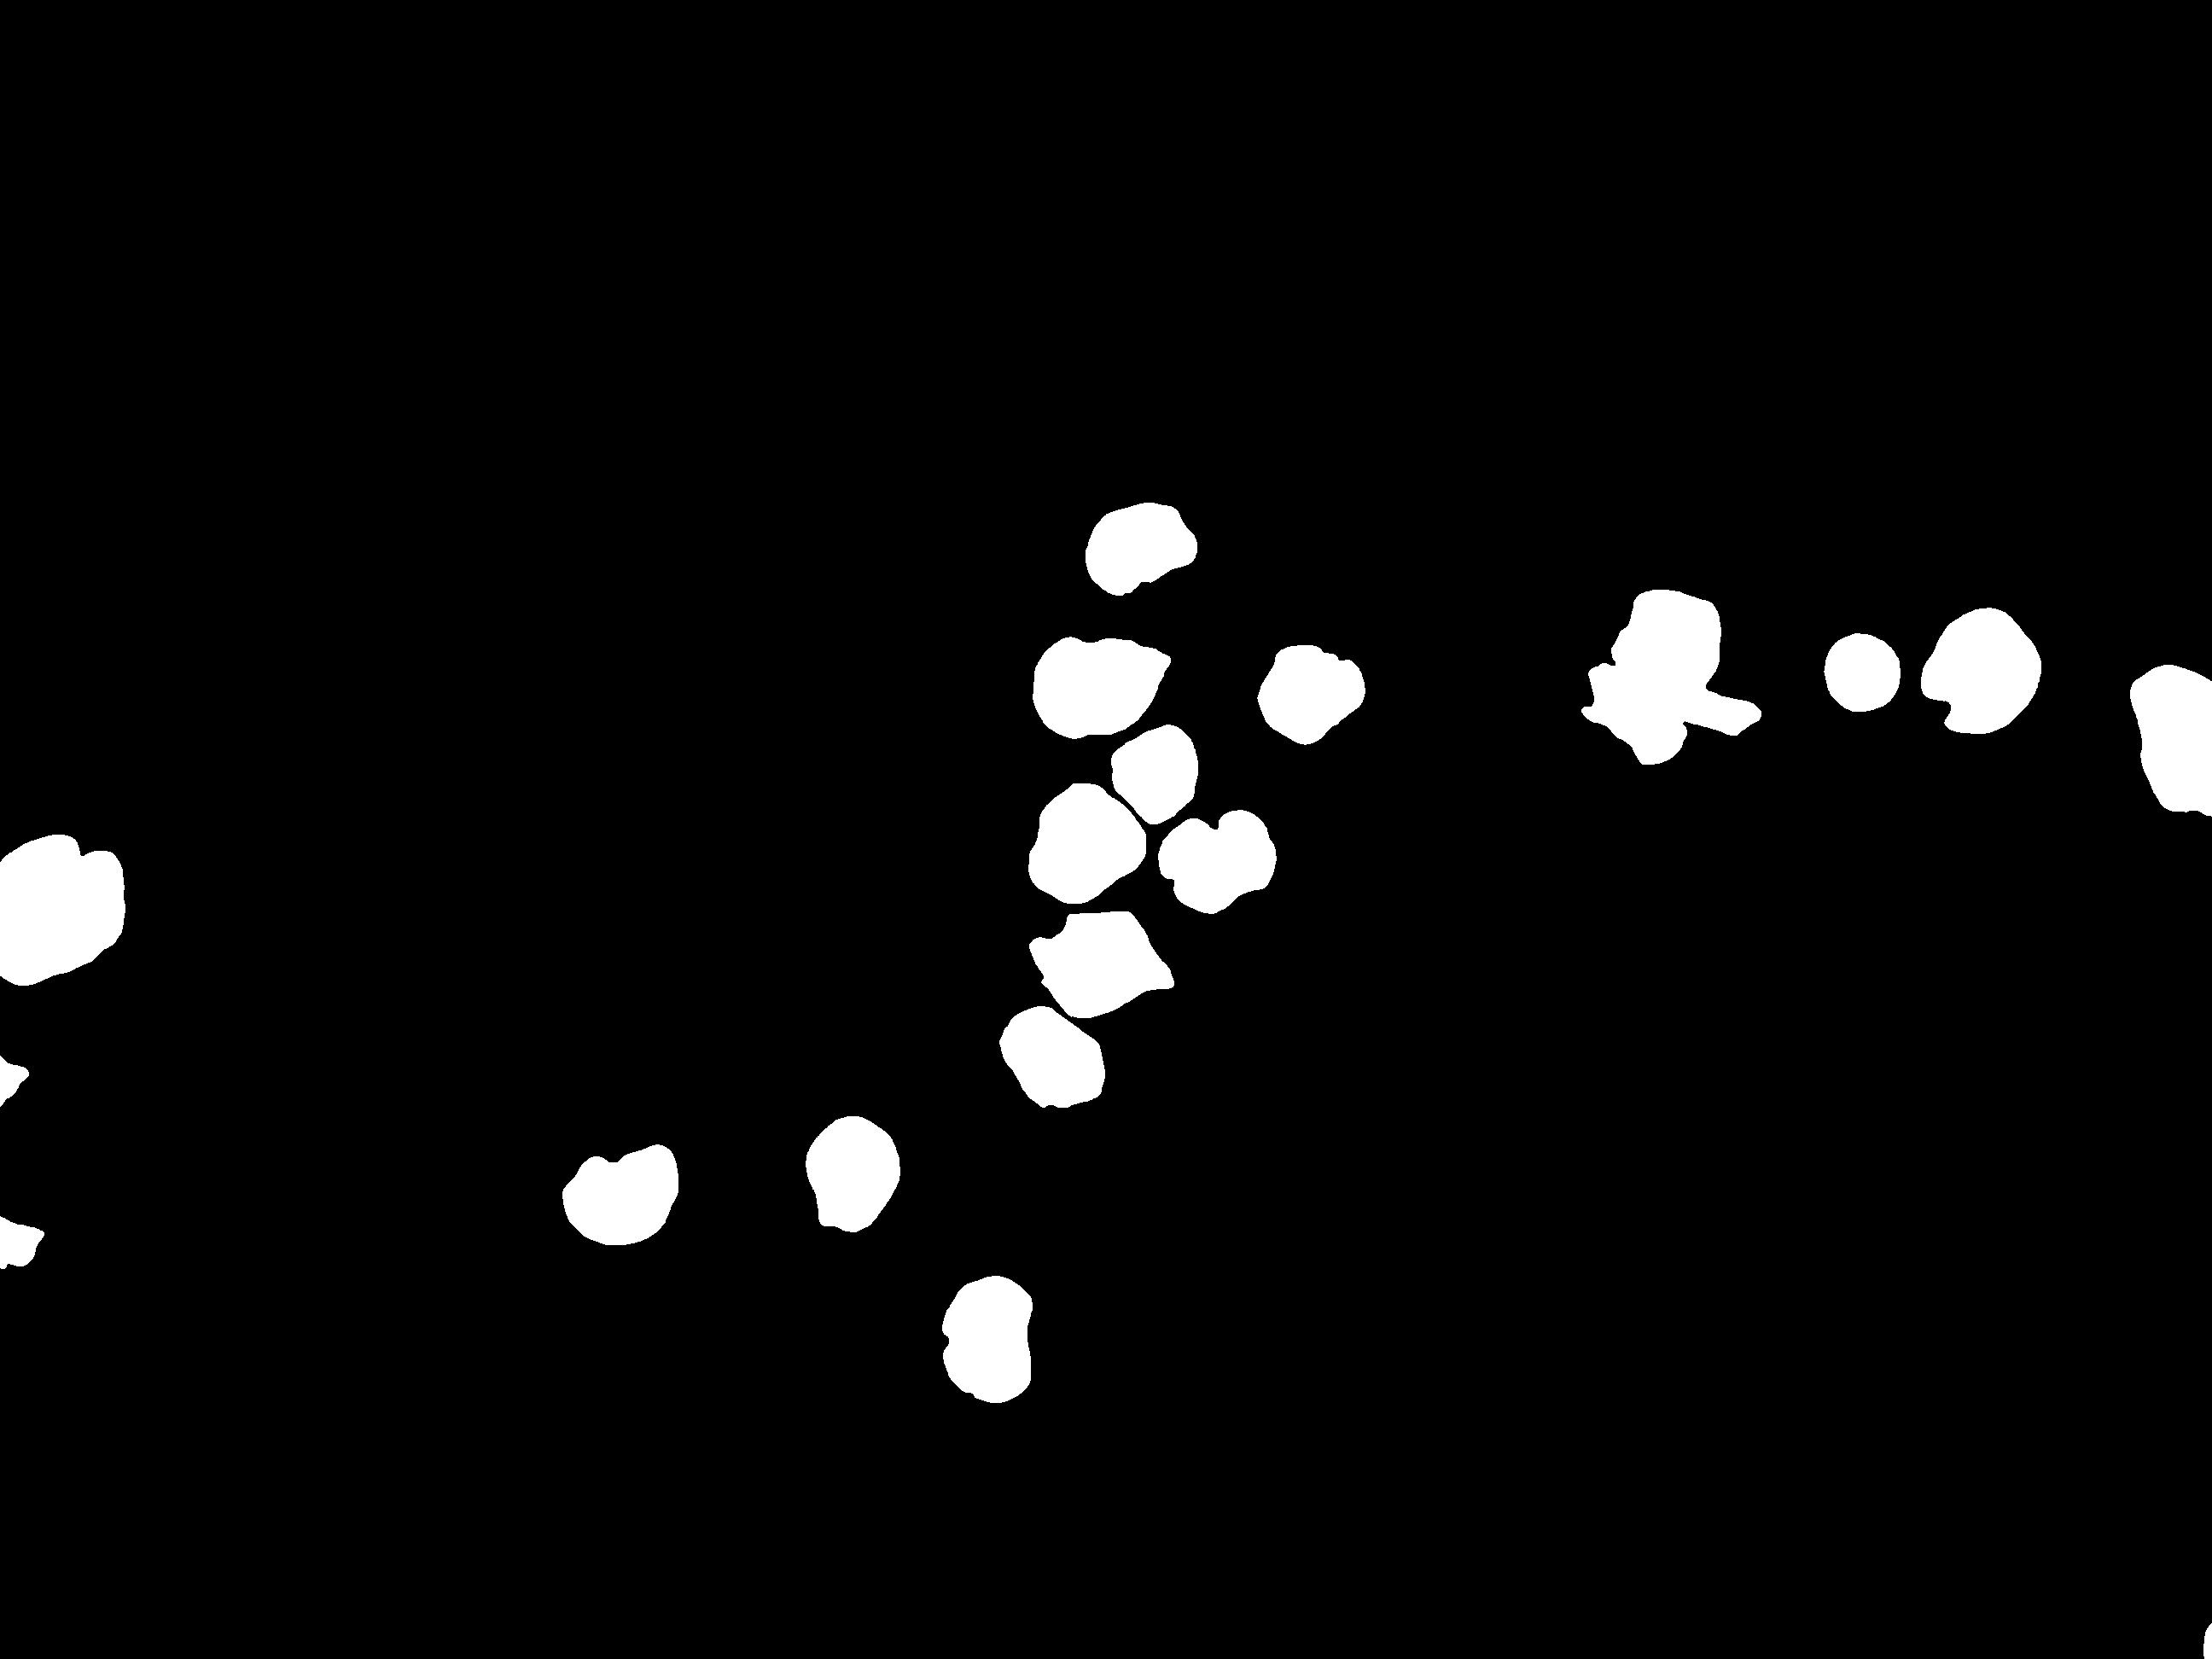
\includegraphics[width=0.24\textwidth]{images/Im050_1_WBCn}
	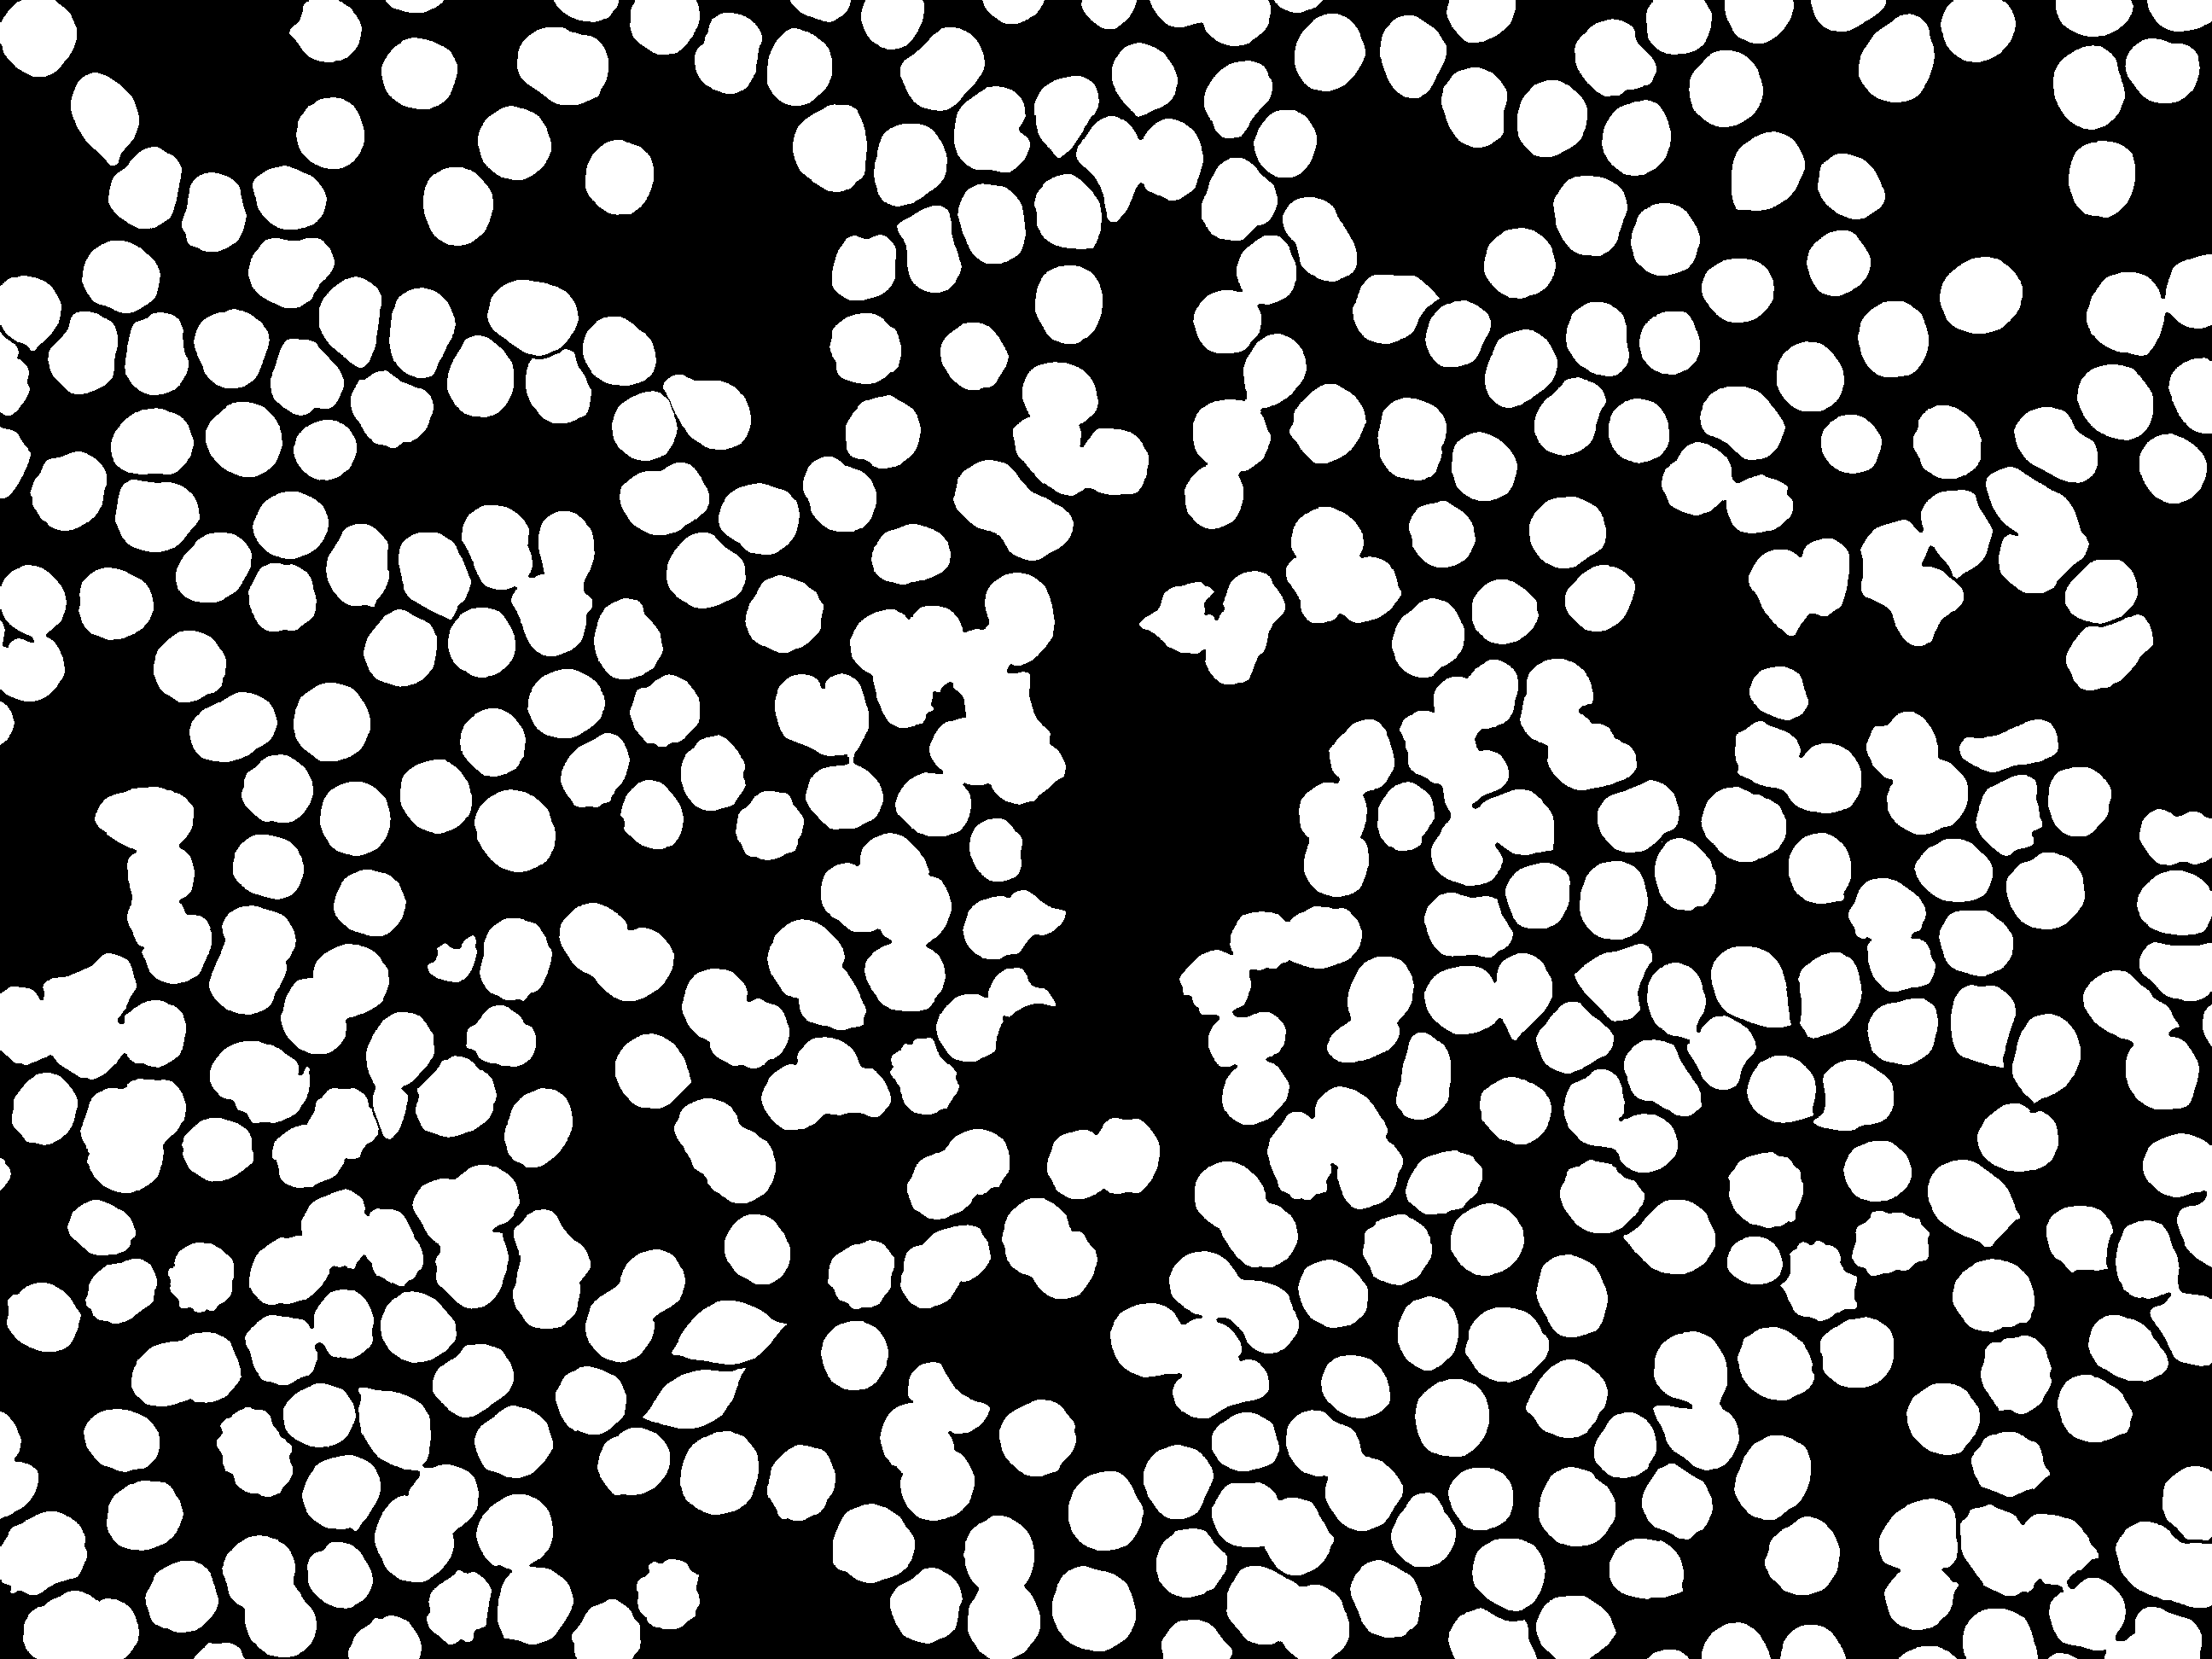
\includegraphics[width=0.24\textwidth]{images/Im050_1_RBC}
	\caption[ALL-IDB1 and relative ground-truths.]{\label{fig:datasetgt1}From left to right: original images from the ALL-IDB1 database, ground-truth for whole leukocyte, only nuclei and RBCs}
\end{figure}

\begin{figure}[ht]
	\centering
	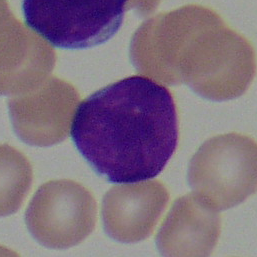
\includegraphics[width=0.16\textwidth]{images/Im035_1}
	
\includegraphics[width=0.16\textwidth]{images/Im035_1_WBC}
	
\includegraphics[width=0.16\textwidth]{images/Im035_1_WBCn}
	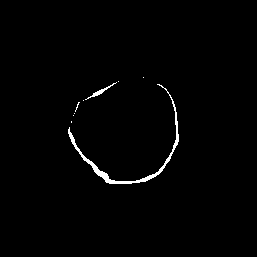
\includegraphics[width=0.16\textwidth]{images/Im035_1_WBCc}
	
	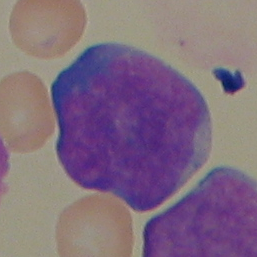
\includegraphics[width=0.16\textwidth]{images/Im091_1}
	
\includegraphics[width=0.16\textwidth]{images/Im091_1_WBC}
	
\includegraphics[width=0.16\textwidth]{images/Im091_1_WBCn}
	
\includegraphics[width=0.16\textwidth]{images/Im091_1_WBCc}
	\caption[ALL-IDB2 and relative ground-truths.]{\label{fig:datasetgt2}From left to right: original images from the ALL-IDB2 database, ground-truth for whole leukocyte, only nucleus and only cytoplasm}
\end{figure}

To evaluate the segmentation performances of the proposed method, 52 images belonging to the ALL-IDB1 have been manually segmented by skilled operators, creating four ground-truth images for each sample. One for the entire WBCS, one for the whole of the RBCs, one for WBCs nuclei and, finally, one for WBCs cytoplasm. Fig.~\ref{fig:datasetgt1} shows some images belonging to the ALL-IDB1 and their relative ground-truth images. Ground-truth images have also been extracted for images belonging to the ALL-IDB2, but in this case, the manual segmentation is only devoted to the analysis of leukocytes, so the ground truth images display only the cytoplasm and the nucleus of the leukocyte, as it can be seen in Fig.~\ref{fig:datasetgt2}.
Despite our main efforts are devoted in designing a method able to achieve a robust segmentation with different image datasets, in our previous works \cite{Put15c, Put15d}  just the ALL-IDB dataset has been used, mainly because the proposed approach exploited the subdivision of the ALL-IDB dataset. Indeed, the ALL-IDB2 images were used to create the training set, being able to develop a robust model to segment optimally the original images in ALL-IDB1. Our aim has always been to let our segmentation algorithm work for different kinds of images and, consequently, different datasets. 
For this reason, two more datasets have been used for testing the proposed method. 
IUMS-IDB is provided by the Iran University of Medical Science \cite{Sarrafzadeh}. It presents 100 microscopic images of size $732 \times 572$, taken from peripheral blood of 8 healthy subjects. These images are truly different from the ones present in the ALL-IDB, since the microscope slides have been smeared and stained with a different staining technique. SMC-IDB, on the other hand, has been proposed in \cite{Mohamed}, presented at IEEE's 2012 SMC conference. It has been acquired from slides stained with the same staining technique as ALL-IDB. Nevertheless, the images are different, since they have been acquired with a different combination of microscope and camera. This dataset provides a total of 367 peripheral blood images of size $640 \times 480$.
Sample images taken from IUMS-IDB and SMC-IDB are shown in \ref{fig:datasets_samples}.

\begin{figure}[h]
	\centering
	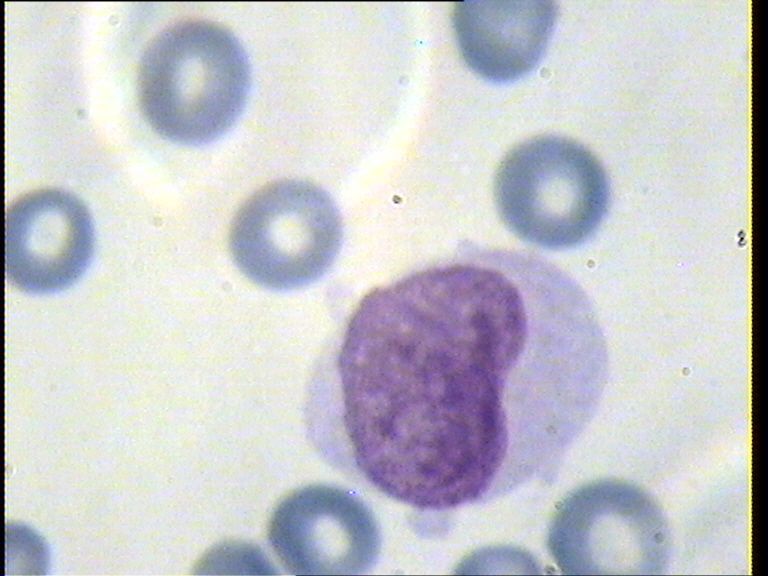
\includegraphics[height=0.33\textwidth]{images/2016_1_mva/IUMS}
	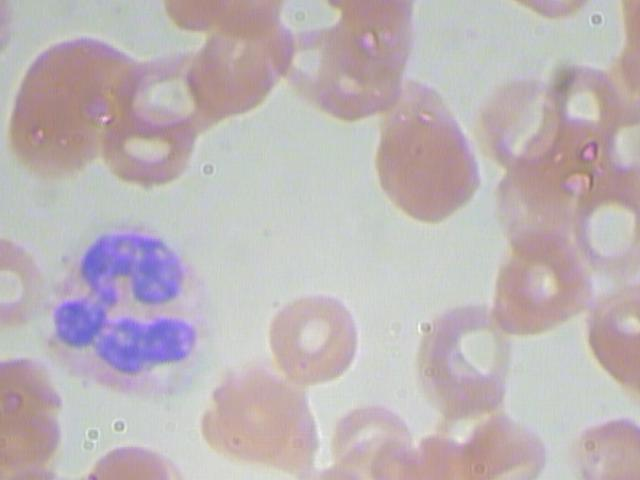
\includegraphics[height=0.33\textwidth]{images/2016_1_mva/SMC}
	\caption[IUMS-IDB and SMC-IDB samples.]{\label{fig:datasets_samples}From left to right: sample image from IUMS-IDB and SMC-IDB.}
\end{figure}

\newpage
\section{Malaria}
\label{malaria_survey}
This chapter explains in detail the characteristics of malaria disease in general, how it is caused, how it affects humans and, finally, the details of malaria parasites. It refers the survey work \cite{Loddo2018}.
Malaria is an epidemic health disease so rapid and accurate diagnosis is necessary for proper intervention. 
Human malaria infection is not strongly related to cell count, but it needs different tests in order to be identified. It can only be caused by parasitic protozoans belonging to the \emph{Plasmodium} type. The parasites are spread to people through the bites of infected female Anopheles mosquitoes, called "malaria vectors".
There are five parasite species that cause malaria in humans and two of these species, \emph{Plasmodium falciparum} and \emph{Plasmodium vivax}, constitute the greatest threat. \emph{Plasmodium~ovale}, \emph{Plasmodium malariae} and \emph{Plasmodium knowlesi} are the three remaining species that are less dangerous in humans \cite{WHO_dec_2016}, as shown in Figure \ref{fig:malaria_types}.
All five species may appear in four different life-cycle stages during the infection phase in peripheral blood: ring, trophozoite, schizont, and gametocyte. Some examples are shown in Figure \ref{fig:malaria_stages}.
The life-cycle-stage of the parasite is defined by its morphology, size and the presence or absence of malarial pigment.
The species differ in the changes of infected cell's shape, the presence of some peculiar dots and the morphology of the parasite in some of the life-cycle-stages \cite{Somasekar2011}.

\begin{figure}[h]
	\centering
	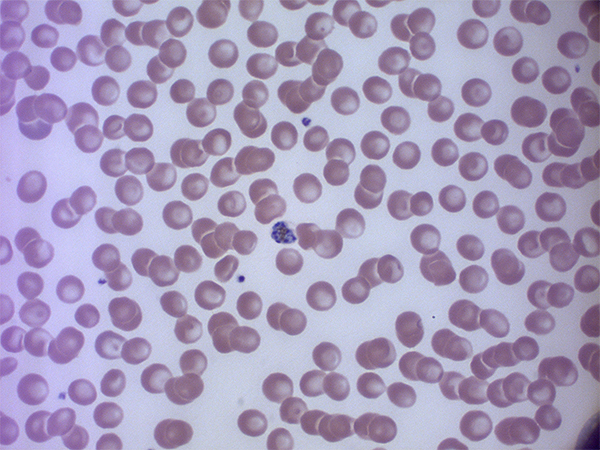
\includegraphics[width=0.48\textwidth]{images/malaria/f2_Pfalciparum}\vspace{1 mm}
	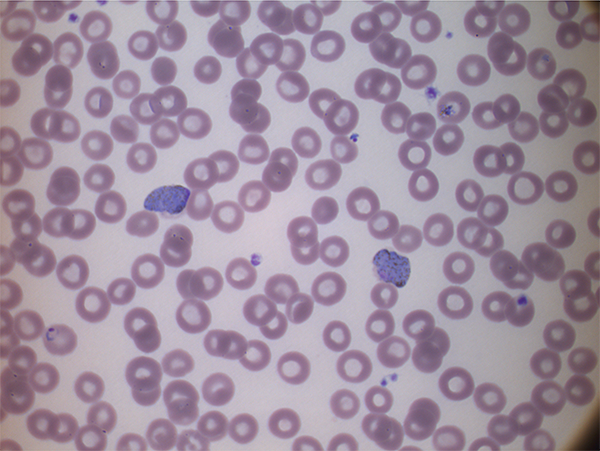
\includegraphics[width=0.48\textwidth]{images/malaria/f2_Pvivax}
	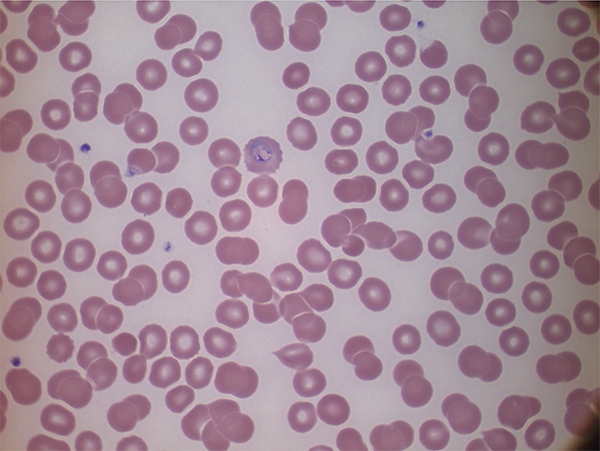
\includegraphics[width=0.48\textwidth]{images/malaria/f2_Povale}
	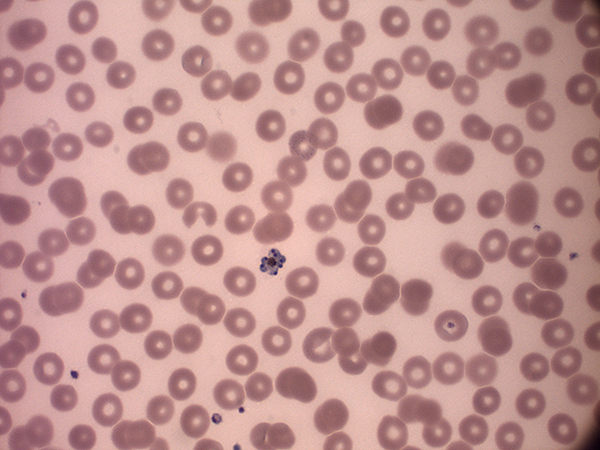
\includegraphics[width=0.48\textwidth]{images/malaria/f2_Pmalariae}
	\caption[Human malaria parasites.]{\label{fig:malaria_types}Types of human malaria parasites: from left to right, \emph{P. falciparum} in its schizont stage, \emph{P. vivax} in two gametocytes specimens and one ring stage, \emph{P. ovale} in its ring stage, \emph{P. malariae} in its schizont stage.
		Courtesy of CHUV, Lausanne.}
\end{figure}

\subsection{Related Works}
% Pre Processing starts
In an image analysis field, especially when we refer to complex computer-aided pipelines, preprocessing methods are particularly used to improve the image data by suppressing unwanted noise or enhancing some image features for further processing.
It is worth mentioning preprocessing methods because they are an essential step regarding the image analysis field, but, for what concerns the malaria-affected blood image analysis, in our review, we mainly found methods that operate for illumination correction and noise filtering purposes.
Generally speaking, digital~microscopy images can be acquired in different lighting conditions, with several types of acquisition devices or from blood smears stained with various staining protocols, and, consequently, the features of similar images could differ a lot.
Different techniques for illumination correction have been suggested to reduce such variation, e.g., a lot of authors work with grayscale-converted images as an illumination correction method.
On the other hand, noise filtering aims to remove the noise introduced by mishandling the slides and the camera settings.
Morphological operators have been extensively used as preprocessing for image enhancement in significant studies.
Erosion and dilation operations on raw smear images allow for discarding undesired patterns and help in the selection of required cells or regions of interest. Morphological operators are useful for the removal of unwanted
objects, holes filling, splitting, thinning and thickening. Different researchers during the automated diagnosis of malaria used morphological operations in the preprocessing phase, and the most recent are listed below.

In \cite{Gonzalez2016}, Gonzalez-Betancourt et al. proposed a system to determine markers for watershed segmentation based on the Radon transform and mathematical operators. In the first step of the process, small irrelevant structures and part of the noise are eliminated by a morphological filter, in~order to ensure the preservation of the edges of the cell. Image smoothing is performed by a morphological erosion-reconstruction and dilation--reconstruction filter with a disk structuring element of a radius equal to 20 pixels, which is $0.274$ times smaller than the average radius of the RBCs. 

In this way, the influences of the size and the shape of the structures can be separated in the smoothing process. At the same time, the objects that are not eliminated remain unchanged. Besides, a morphological closing is performed with a disk structuring element having a radius smaller than half the average of the RBCs radii, to connect the possible (more than one) markers that can appear on a single cell.

In \cite{Kareem2012}, Kareem et al. illustrated a morphological approach for blood cell identification and used image features such as intensity, histogram, relative size and geometry for further analysis. Before~the identification of blood cells, the authors propose different morphological filtering based on the size of RBCs for platelets and artifacts elimination. Dilation is performed by a concentric ring structuring element and erosion by a disk-shaped structuring element. The radius of the structuring element depends on the radius of the RBCs so that all the components smaller than the RBCs can be removed.

The system proposed in \cite{Oliveira2017} by Oliveira et al. is based on image processing, artificial intelligence techniques, and an adapted face detection algorithm to identify Plasmodium parasites. The latter uses the integral image and haar-like features concepts, and weak classifiers with adaptive boosting learning. The search scope of the learning algorithm is reduced in the preprocessing step by removing the background around blood cells employing morphological erosions both for training and for testing.

Romero-Rondon et al. in \cite{Romero2016} presented an algorithm that uses morphological operations, the watershed method, the Hough transform and the clustering method of k-means to detect overlapped RBCs. In the preprocessing stage, white blood cells and platelets are removed before the segmentation task. During this step, some noise, the WBC cytoplasm, and platelets remain on the image. 
Therefore, the small objects are removed using a morphological opening, and then the image is dilated with a disk-shaped structuring element.

Reni et al. in \cite{Reni2015} described a new algorithm for morphological filtering of the blood images as a preprocessing tool for segmentation. Conventional morphological closing on blood images removes the unwanted components but also useful information. On the contrary, the proposed method preserves the necessary knowledge of foreground components while eliminating noise and artifacts.

In the method proposed in \cite{Sheik2013} by Sheikhhosseini et al., the first phase is the stained object extraction that detects candidates' objects that can be infected by malaria parasites using intensity and color. Before detecting the stained objects, the method firstly extracts the foreground. The foreground image is a binary image that is produced after applying morphological hole filling on such pixels that have lower intensity value than average intensity value of the green layer. After the stained objects' extraction process, a series of morphological operations are also employed to eliminate small components and complete the final stained objects.

An edge-based segmentation of erythrocytes infected with malaria parasites using microscopic images is proposed by Somasekar et al. in \cite{Somasekar2015}.  A fuzzy C-means clustering is applied to extract infected erythrocytes, which is further processed for the final segmentation. A morphological erosion is used to erase some small noises and spots before the segmentation and holes inside the infected erythrocytes are filled using a morphological hole filling operation for the final segmentation.

In \cite{Tek2010}, Tek et al. presented a complete framework to detect and identify malaria parasites in images of Giemsa stained thin blood film specimens. In addition, the system is able to identify the infecting species and life-cycle stages.
The preprocessing step of the proposed method is applied to reduce the variations in the observed size, intensity, and color of the cells and stained objects before the detection and classification steps. The aim is to correct the non-uniform illumination in the images. The estimation is based on a morphological closing operation using a sufficiently large structuring element. Enough large size for an input image is determined automatically concerning its average cell size computed from the area granulometry distribution.

The median filter is often used for reducing impulse noise. Several studies have used it to enhance microscopic images of peripheral blood smear towards the characterization of malaria followed by adaptive or local histogram equalization. Local low pass filter and local adaptive histogram equalization techniques have also been applied to enhance the pathological image quality. Das et al. \cite{Das2015} showed that the geometric mean filter provides better performance towards improving peripheral blood smear images. Di Ruberto et al. \cite{DiRuberto2016} proposed an approach to overcome the problem of uneven illumination conditions in image acquisition. For this purpose they designed an illumination pattern that simulates the classic visual defects introduced by the digital microscope lenses, that is the vignetting effect. Starting from the smallest radius, they applied different illumination patterns, created modifying the radius of the Gaussian curve, to the original images. Then, a similarity value measures the difference regarding pixels between the original images and the corrupted ones.
% Pre Processing ends

% Segmentation starts
Segmentation is a critical step in image analysis because it permits the identification and separation of the regions that compose an image, according to specific criteria of homogeneity and separation. Its~main target is to divide the image into parts that have a strong correlation with objects or areas of the real world contained in the image.
The commonly used segmentation methods essentially operate considering characteristics such as the brightness value, colour, and reflection of the individual pixels, identifying groups of pixels that correspond to spatially connected regions. As for many problems of image processing, there is no standard solution valid in general. Therefore different segmentation techniques can be applied, according to the characteristics of the images to process and of the objects to segment.
Medical images segmentation is typically performed using two main strategies: the first level aims to separate whole cells or tissues from the background and the second one seeks to separate the tissue structure in different regions or the cell in their components, as the nucleus from the cytoplasm or intracellular parasites. The latter case is commonly used in applications in which the cell class depends on the morphological characteristics of its components.

%%% THRESHOLDING METHODS
Several other authors attempted to use thresholding combined with morphological operations as a segmentation method in their computer-aided systems, and they are described as follows.

Arco et al. in \cite{Arco2014} worked on thick blood films and proposed a method that uses an adaptive thresholding based scheme, which also allows a valid classification of pixels. This means that the election of whether a pixel belongs to the background or the signal (parasites and white blood cells) is only established by the pixels around it, that is its neighborhood. Then, morphological methods are applied to evaluate the area of connected components, labeling those belonging to parasites and counting their number.

Anggraini et al. \cite{Anggraini2011} proposed a method for separating blood cells, parasites and other components from the background in a microscopic field of a thin blood smear. They applied several global thresholding methods and visually compared the results to determine which technique yields the best result qualitatively. The binary image was then subjected to a hole filling morphological operator and applied as a marker to label blood cells. From each identified cell (RBC and WBC), constituents of the parasite (nucleus and cytoplasm) were extracted using multiple thresholds.

Dave et al. in \cite{Dave2017} performed image segmentation using histogram-based adaptive thresholding followed by mathematical morphological operations (erosion and dilation). The detection of infected RBCs is based on an unsupervised learning technique.

The automated method proposed in \cite{Elter2011} by Elter et al. for parasite detection and identification worked on thin blood film acquired with Giemsa stain. The authors found that the G and B channels of the RGB color are outstanding features to identify objects containing chromatin in Giemsa stained blood films are considered highly discriminative and also almost independent of differences in illumination and staining intensity. They transformed the colour input image into a monochrome image \textit{I(x,y)}, which highlights objects containing chromatin: $ I(x,y) = arctan \frac{I_{green}(x,y)}{I_{blue}(x,y)} $. In this work, mathematical morphology has been used with a black top-hat operator to separate MP from both leukocytes and platelets, with a non-flat paraboloid structuring element with a radius of 9 and a slope of one~pixel. It should be taken into account that these fixed parameters might not be suitable for images with different pixel resolutions. A thresholding operation follows the black top-hat operator with a fixed threshold, which, according to the authors, is reliable given the independence of the G and B channels concerning illumination and staining intensity. However, the authors do not define the value of this fixed threshold in their paper.

Kareem et al. in \cite{Kareem2011} used the Annular Ring Ratio transform method. Before applying it, a~preprocessing phase for removing platelets, parasites and other artifacts in the image has been performed. In the proposed method, the image after being converted to grayscale undergoes a morphological opening similar to closing. Unlike conventional closing (dilation followed by erosion), which uses the same structuring element, two different structuring elements are used: a concentric ring for dilation and a disk for erosion. The inner and outer diameter of the dilation ring is set to 35\% and 70\% of RBCs size, respectively, and the erosion disk has the same diameter. Therefore, considering that fixed manually defined parameters are used for this strategy, the results may substantially differ depending on the image resolution. This approach results in locating only the stained components in the image instead of all the cells and hence will not only speed up the operation but reduce the~complexity.

Mushabe et al.~\cite{Mushabe2013} used morphological and statistical classification to detect malaria in blood smears by identifying and counting red blood cells and Plasmodium parasites. Morphological~operations and histogram-based thresholding are used to extract RBCs, and boundary curvature calculations and Delaunay triangulation are used for splitting clumped RBCs. They worked on Giemsa-stained thin blood smears.

In \cite{Ross2006}, Ross et al. proposed a method that provides a positive or negative diagnosis of malaria and differentiates parasites by species. The segmentation step relies on a six-step thresholding selection strategy. It aims to identify and segment potential parasites and erythrocytes from the background. Mathematical morphology has been used in several key steps of the procedure. Hole~filling is used in the first step to fill RBCs' binary masks obtained from first thresholding. \mbox{Afterwards, step 4} employs RBCs' morphological reconstruction with parasites' mask, found in step 2, for identifying infected cells. In step 5, a morphological opening filter, using a disk-shaped SE with a radius equal to the mean erythrocyte radius less the standard deviation, is applied to the grayscale, morphologically filtered, green component to remove any objects smaller than an erythrocyte. The morphological gradient (the difference between dilation and erosion of the image) is then calculated using a diamond-shaped SE with unity length.
Finally, in step 6, the intersection of morphological gradient image and the dilated cell cluster is calculated. This image is then transformed into a binary image by thresholding any value greater than zero. A series of morphological operations, namely a closing operation, thinning, and spur-removal are then applied to generate a contour of the segmented erythrocytes. Contours are filled, and the segmented mask is again reconstructed with the correct parasite marker image to result in a segmented mask of infected cells. RBCs and parasites masks are consequently ready for the next generation step.

Savkare et al. \cite{Savkare2011b} worked on thin blood films with Giemsa staining and used a global threshold and Otsu threshold \cite{Otsu} on the grayscale enhanced image (green channel) for separating foreground from background. Hole filling has been performed on identified cells, and morphological operators have been used to identify overlapping cells. Then, a watershed transform has been applied for separating overlapped cells.

Besides, in the method proposed in \cite{Somasekar2017} by Somasekar et al., the segmentation of the infected parasites is based on thresholding. It is achieved in two stages by maximizing the between-class variance of an original image and consequently by an iterative threshold selection from a stage-one threshold image with suitable stopping criteria. The segmented results are post-processed to improve the accuracy of malaria parasites detection by morphological operators (erosion and closing).

% Morphology and granulometry in Segmentation stage:
On the other hand, a lot of works have been realized through mathematical morphology and granulometry in the segmentation stages, even in combination with thresholding strategies. They are briefly analyzed below.

Ahirwar et al. \cite{Ahirwar2012} based their approach on thresholding and granulometry. The histogram of the complemented green component has been used, and it is said to be a bimodal distribution in all the considered images. Then, both local and global thresholds are used, and the union of the two binary images is chosen as the parasite marker image. A morphological opening filter, using a disk-shaped SE with a radius equal to the mean erythrocyte radius less the standard deviation, is applied to the grayscale morphologically filtered green component of the image to remove any objects smaller than an erythrocyte. The morphological gradient is then calculated using a diamond-shaped SE with unity length. The segmentation method is applied to each object in the reconstructed binary image of erythrocytes individually. Those objects that do not exceed the area of a circle with a radius equal to the mean erythrocyte radius plus the standard deviation are regarded as being single cells and are unmodified.
On the other hand, the clumped cells are segmented as follows. First, the intersection of the morphological gradient image and the dilated cell cluster is taken. This image is then transformed into a binary image by thresholding any value greater than zero. A series of morphological operations, namely a closing operation, thinning, and spur removal is then applied to generate a contour of the segmented erythrocytes. The contours are filled, and the segmented mask is again reconstructed with the correct parasite marker image to result in a segmented mask of infected cells.

Di Ruberto et al. \cite{DiRuberto2002} aimed to detect the parasites utilizing automatic thresholding based on a morphological approach applied to cell image segmentation, which is more accurate than the classical watershed-based algorithm. They applied grey scale granulometries based on opening with disk-shaped elements, flat and hemispherical. They used a hemispherical disk-shaped structuring element to enhance the roundness and the compactness of the red blood cells improving the accuracy of the classical watershed algorithm, while they used a disk-shaped flat structuring element to separate overlapping cells. These methods make use of the red blood cell structure knowledge, which is not used in existing watershed-based algorithms.

Khan et al. in \cite{Khan2011} presented a novel threshold selection technique used to identify erythrocytes and possible parasites present on microscopic slides that dramatically benefit from morphological operations, such as granulometry and morphological reconstruction.

In \cite{Rosado2017}, Rosado et al. proposed a system using supervised classification to assess the presence of malaria parasites and determine the species and life cycle stage in Giemsa-stained thin blood smears. For the RBCs segmentation, they used an adaptive thresholding approach followed by a closing morphological operation with an elliptical structuring element.

Soni et al. \cite{Soni2011} performed segmentation of erythrocytes by using granulometry as well. The~size and eccentricity of the erythrocytes are also required for the calculation of some feature values (as~these can be indicative of infection). The shape of the objects (circular erythrocytes) is known a priori, but the image must be analyzed to determine the size distribution of objects in the image and to find the average eccentricity of erythrocytes present.
Grayscale granulometries based on opening with disk-shaped elements are then used. Non-flat disk-shaped structural elements are applied to enhance the roundness and compactness of the red blood cells and flat disk-shaped structural elements applied to segment overlapping cells. The object to be segmented differs significantly in contrast to the background image. Changes, in contrast, can be detected by operators that calculate the gradient of an image. The gradient image can be computed, and a threshold can be applied to create a binary mask containing the segmented cell. The binary gradient mask is dilated using a vertical structuring element followed by a horizontal structuring element. The cell of interest has been successfully segmented, but~it is not the only object that has been found. Any objects that are connected to the border of the image can be removed.

In Tek et al. \cite{Tek2010}, the localization of the parasites is achieved after a foreground and background segmentation step. Firstly, a rough foreground image using morphological area top-hats (using the average cell area value) is extracted. Then, from these rough foreground and background regions, two different threshold values are determined and used in morphological double thresholding of the input grey level image to produce a refined binary foreground mask. From the foreground image, the stained pixels are detected using a thresholding approach again and finally used as markers to extract the stained objects by morphological area top-hats based on the estimated average area value.

In \cite{Yunda2012}, Yunda et al. proposed a method for \textit{P. vivax} parasite detection. The segmentation phase is a combination of border and region detection that allows rejection of the image background and permits identifying each of the objects. Initially, the morphological gradient method is used to enhance the borders of previously found objects. It is followed by a threshold detection stage using the K-Median method.
Furthermore, a Laplacian operator was used to discriminate the pixels that are interior or exterior concerning the regions of the images and then erosion operation followed by two dilations were applied to delete the pixels that did not make part of any object. In the end, Absence~of Gradients and Nernstian Equilibrium Stripping (AGNES) and K-Median techniques were applied to assign the remaining number of pixels to each region, using the image regions previously identified as objects and background as the starting point.

Several authors used marker-controlled watershed \cite{Soille2004} with the morphological approach, as~described in the following.

Das et al. in \cite{Das2011, Das2013, Das2014, Das2015} segmented erythrocytes as aforesaid and then morphological operators are used to eliminate unwanted cells like leukocytes and platelets. Moreover, overlapping erythrocytes are segmented by using a marker-controlled watershed segmentation technique.

In \cite{Devi2017}, Devi et al. proposed a computer-assisted system for quantification of erythrocytes in microscopic images of thin blood smears. The performance of the system in classifying the isolated and clump erythrocytes by geometric features is evaluated for the different classifiers. The clump erythrocytes are segmented using marker-controlled watershed with h-minima as an internal marker.

In \cite{Dey2015}, Dey et al. presented an automatic system for segmenting platelets, useful for identifying the disease like malaria, using a color based segmentation and mathematical morphology (opening~operations with a disk element of radius 2).

In the study presented in \cite{Diaz2009} by Diaz et al. for quantification and classification of erythrocytes in stained thin blood films infected with \textit{Plasmodium Falciparum}, the authors used connected morphological operators in the segmentation step. The RBCs are detected as follows: firstly, a pixel classification allowed for labeling each image pixel as either background or foreground, based on its color features. Afterward, an inclusion-tree structure is used to represent the hierarchical object relations between background and foreground so that a filtering process allows for removing irrelevant structures such as artifacts generated at the staining or digitization processes.

Khan et al. \cite{Khan2011}, among other experimentations, used it to try to separate overlapping cells because, according to their statements, the watershed transform can isolate touching cells, but it is not sufficient for overlapping cells.

In the algorithm described by Romero-Rondon et al. in \cite{Romero2016}, the detection of overlapped RBCs is still based on marker-controlled watershed transform. To define the suitable markers in the watershed transform, they used three different approaches, based on a morphological erosion operation, on Hough transform and on a clustering method of K-means.

{Savkare et al. in \cite{Savkare2015} segmented cells using K-mean clustering and global threshold. Overlapping cells are separated using a Sobel edge detector and watershed transform, applied to each cluster separately. Over-segmentation is minimized by a series of morphological operations, like erosion and dilation, utilizing disk-shaped structuring elements.
	
	In \cite{Savkare2011a}, an approach to detect red blood cells with the following classification into parasite infected and healthy cells for further estimation of parasitemia is proposed. For separation of overlapping cells, the watershed transform is applied on a distance transform of a binary mask of cells having a larger area.
	
	In \cite{Springl2009}, {\v{S}}pringl performed red blood cell segmentation by using marker-controlled watershed transformation based on the image gradient. Markers are computed as a combination of the binary mask of the red blood cells and centers of the cells that are computed using a similar algorithm that was utilized for the evaluation of the average cell radius. The binary mask is obtained by thresholding the grayscale image with an automatically estimated threshold using the Otsu method \cite{Otsu}.
	
	In \cite{Sulist2015}, Sulistyawati et al. combined morphological operations (erosion, dilation, opening, and closing) and blob analysis to segment and identify malaria parasites with a high degree of accuracy.
	
	Tek et al. in \cite{Tek2006} proposed a classifier-based method for the segmentation stage, which relies on a Bayesian pixel classifier to distinguish between stained and non-stained pixels. In particular, they used a non-parametric approach based on histograms to produce the probability density functions of stained and non-stained classes. Stained pixels can belong to other components such as WBCs, platelets or artifacts, in addition to the parasites, and so the detection procedure requires a further classification to distinguish among parasite and non-parasite pixels. However, the stained pixels have to be represented as connected sets, representing stained objects, to extract features for the classifier. Furthermore, top-hat extraction and infinite reconstruction were applied to find the regions that include the objects.
	
	% Segmentation ends 
	
	% Feature extraction starts
	Feature extraction has the aim of reducing the computational complexity of the subsequent process and facilitating a reliable and accurate recognition for unknown novel data, considering~that the input data to an algorithm could be too large to be processed, and it could be redundant (e.g., the repetitiveness of pixels patterns in an image). Moreover, the in-depth understanding of the domain-specific knowledge gained by human experts on the problem being addressed can be of extreme importance for the design of a reliable and effective feature extraction engine \cite{Jiang2009}.
	It starts by determining a subset of the initial features, and this procedure is called feature selection. The~selected features are expected to contain the relevant information from the input data so that the desired task can be performed by using this reduced representation instead of the complete initial data.
	Malaria parasite infection causes microstructural changes in erythrocytes. The microscopic features of the RBCs are usually specific to morphology, intensity, and texture. They may also represent the differences that occur among healthy and unhealthy cells. Most of the studies have reported both textural and geometric features for describing malaria infection stages \cite{Das2015}.
	Generally speaking, features may be distinguished according to the following characteristics: morphological features and textural and intensity features.
	
	It is a well known mathematical morphology approach to compute a size distribution of grains in binary images, using a series of morphological opening operations. It is the basis for the characterization of the concept of size. Some authors used area granulometry for preprocessing purposes in malaria characterization \cite{Tek2010}, even though it is certainly effective for extracting cell size features' information \cite{Springl2009, Tek2006, Malihi2013}. In \cite{Tek2010}, local area granulometry combined with the color histogram is used as features. The area granulometry feature is calculated locally on the binary mask of the stained objects, for the RGB channels, and then concatenated. Morphological features are also used in \cite{Ross2006} (erosion dilation), in \cite{Das2011} (opening, closing) and in \cite{DiRuberto2002} (skeleton) to classify parasites.
	% Feature extraction ends
	
	\begin{figure}[!t]
		\centering
		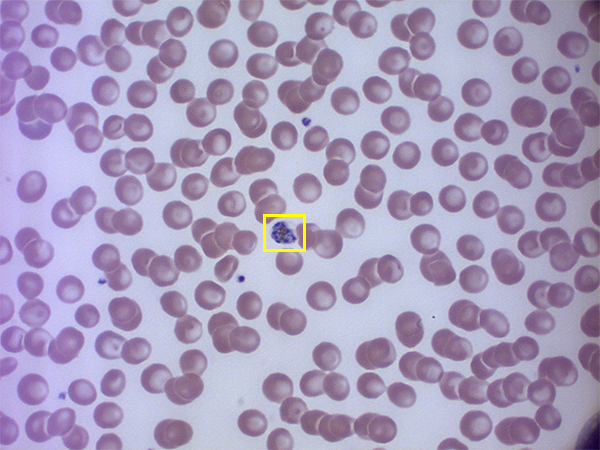
\includegraphics[width=0.48\textwidth]{images/malaria/f2_Pfalciparum_rect}
		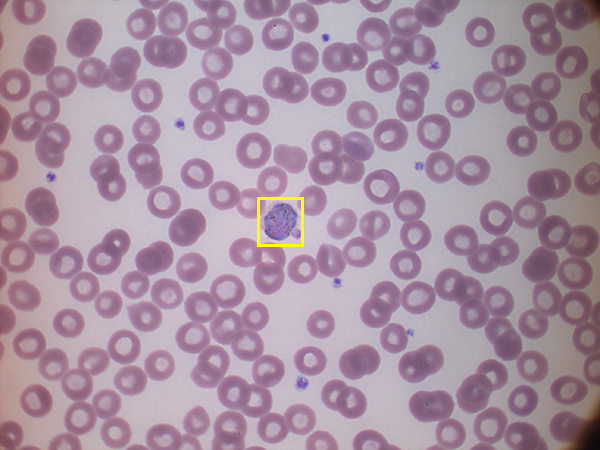
\includegraphics[width=0.48\textwidth]{images/malaria/f2_Pvivax_rect}
		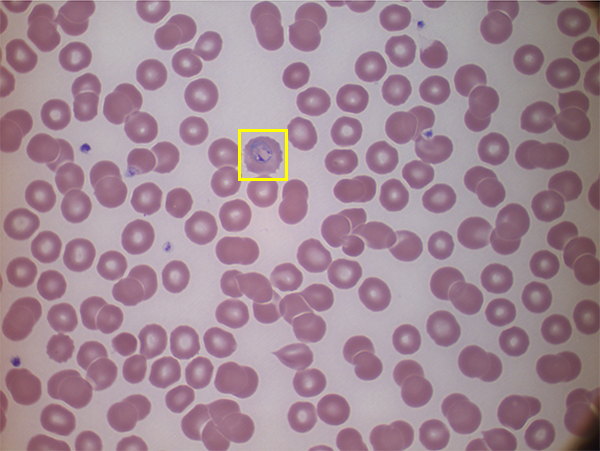
\includegraphics[width=0.48\textwidth]{images/malaria/f2_Povale_rect}
		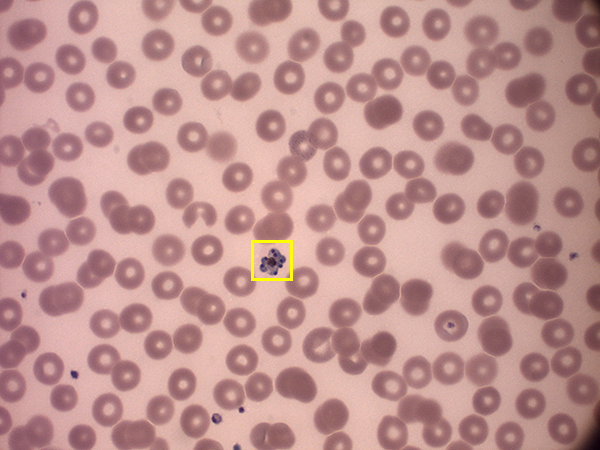
\includegraphics[width=0.48\textwidth]{images/malaria/f2_Pmalariae_rect}
		\includegraphics[width=2cm, height=2cm]{images/malaria/f2_Pfalciparum_crop}
		\includegraphics[width=2cm, height=2cm]{images/malaria/f2_Pvivax_crop}
		\includegraphics[width=2cm, height=2cm]{images/malaria/f2_Povale_crop}
		\includegraphics[width=2cm, height=2cm]{images/malaria/f2_Pmalariae_crop}
		\caption[Malaria parasites.]{\label{fig5_malaria_types}Types of malaria parasites: from top left, clockwise, \emph{P. Falciparum} in its schizont stage, \emph{P. Vivax} in a gametocytes specimen, \emph{P. Malariae} in its schizont stage, \emph{P. Ovale} in its ring stage. All parasites have been surrounded with a yellow box. Underneath, from left to right: crops of P. Falciparum schizont, P. Vivax gametocyte, P. Ovale ring and P. Malariae schizont, taken from the boxes. Courtesy of CHUV, Lausanne.}
	\end{figure}
	
	\begin{figure}[!b]
		\centering
		\includegraphics[width=2cm, height=2cm]{images/malaria/falciparum_1_ring}
		\includegraphics[width=2cm, height=2cm]{images/malaria/falciparum_2_trophozoiteAge}
		\includegraphics[width=2cm, height=2cm]{images/malaria/falciparum_3_schizont}
		\includegraphics[width=2cm, height=2cm]{images/malaria/falciparum_4_gametocyte}
		
		\includegraphics[width=2cm, height=2cm]{images/malaria/ovale_1_ring}
		\includegraphics[width=2cm, height=2cm]{images/malaria/ovale_2_trophozoite}
		\includegraphics[width=2cm, height=2cm]{images/malaria/ovale_3_schizont}
		\includegraphics[width=2cm, height=2cm]{images/malaria/ovale_4_gametocyte}
		
		\includegraphics[width=2cm, height=2cm]{images/malaria/vivax_1_ring}
		\includegraphics[width=2cm, height=2cm]{images/malaria/vivax_2c_trophozoiteDeveloped}
		\includegraphics[width=2cm, height=2cm]{images/malaria/vivax_4_gametocyte}
		\caption[Malaria parasite stages.]{\label{fig6_malaria_stages}Examples of malaria parasite stages. From top left: P.falciparum ring, trophozoite, schizont, gametocyte;
			P.ovale ring, trophozoite, schizont, gametocyte; P.vivax ring, developed trophozoite, gametocyte. \cite{Loddo2018}}
	\end{figure}
	
	\subsection{Malaria parasites morphology}
	A blood smear image, obtained through a microscope, is presented in fig. \ref{fig4_colour}. It typically contains at least three regions of interest: white blood cells (or leukocytes), red blood cells (or erythrocytes) and platelets (or thrombocytes). Two different categories of leukocytes exist granulocytes (composed, in turn, of neutrophils, basophils, and eosinophils).
	On the other hand, leukocytes without granules are called agranulocytes (composed of lymphocytes and monocytes). Erythrocytes do not have any subcategory even though malaria parasites (MPs) can infect them, consequently modifying their shape, morphology or coloration conditions. In particular, fig. \ref{fig5_malaria_types} shows several examples of malaria parasites in their different life stages and type.
	Although MPs infect only RBCs, a blood smear image representing both WBCs (particularly granulocytes) and MPs could be tough to analyze because of the similarities in coloration and shape between parasites and WBC grains, as shown in fig. \ref{fig4_colour}.
	
	\begin{figure}[h]
		\centering
		\includegraphics[width=0.8\textwidth]{images/malaria/f2_typical_bb}
		\caption[Malaria blood smear images.]{\label{fig4_colour} Example of blood smear image acquired with a good coloration and illumination scheme. Three different regions of interest characterize the image: an eosinophil granulocyte on the bottom left (yellow bounding box), a schizont Plasmodium Falciparum on bottom center (green bounding box) and the erythrocytes. Please note that some platelets are also present (blue bounding box). Courtesy of CHUV, Lausanne.}
	\end{figure}
	MP-IDB collects four malaria parasite species: Plasmodium Falciparum, Ovale, Malariae, and Vivax, in four different life-cycle stages: ring, trophozoite, schizont, and gametocyte. Plasmodium Falciparum trophozoite and schizont are very rare, and they are not present in our data collection. A complete set of examples, extracted from the dataset, are shown in fig. \ref{fig6_malaria_stages}. The morphology, the size and the presence or absence of malarial pigment of the parasites define their life-cycle-stage. The species differ in the changes of infected cell's shape, the presence of some peculiar dots and the morphology of the parasite in some of the life-cycle-stages \cite{Somasekar2011}.
	An automated malaria parasites analysis on blood smears usually comprises four different tasks, as follows:
	\begin{enumerate}  
		\item Image preprocessing: the images are normalized in colouration because it can differ a lot from image to image, and the different regions of interest are made the most contrasted possible. 
		\item Segmentation: red blood cells and parasites are separated from the background and white blood cells by using algorithms based on different characteristics of the cells (e.g., shape, color, texture).
		\item Feature extraction: relevant characteristics (e.g., shape, color, texture) are extracted from the different region of interest to train an automatic parasite analyzer.
		\item Classification: several classification schemes can be performed. Hierarchically, cells are classified in red blood cells and white blood cells. Afterward, red blood cells are classified in affected by parasite(s) or not. In the end, parasites are classified in their type and life stage. Parasites potentially can also be present outside the cells. In this case, they should need a more specific and dedicated analysis.
	\end{enumerate}
	
	\chapter{WBCs Segmentation}
	\label{wbcs_segmentation}
	The main purpose of this thesis was to develop a CAD system able to extract appropriate and useful information from blood cell images, acquired employing microscopes, to easily perform activities on them, like the WBCC. One of the main issues to deal with is certainly the management of the different staining techniques and illumination conditions in which the image can be acquired. Datasets presented for WBC analysis show several examples \ref{wbc_datasets}.
	All considered, this chapter presents different methods which takes into account these issues and offers solutions to them. Paragraph \ref{iciap_caip_2015} refers to the works \cite{Put15c}, \cite{Put15d}, while paragraph \ref{visapp2018} refers to the work \cite{Porcu}.
	The proposed solution starts with a segmentation step, which is a crucial step in this procedure because its accuracy dramatically affects both the computational performances and the whole system overall accuracy. However, it is also a challenging problem to manage because of the complex nature of the cells, the low resolution of microscopic images and complex scenes, e.g., cells can overlap each other or cells can have different sizes or shapes. On the other hand, the color and contrast between the cells and the background can vary so often according to the standard, inconsistent staining technique, the thickness of smear and illumination. Although standardization is useful to avoid superfluous differences in the features of similar images, a robust segmentation approach can cope with the described issues, and this is undoubtedly one of the main motivations to the realization of this work.
	State of the art shows that most of the authors proposed traditional methods to perform cells segmentation, like thresholding. In some cases, WBCs counting has been based on detection methods rather than on segmentation ones, by using the circular Hough transform \cite{Mahmood} or texture analysis, even though color image segmentation could also be performed with pixels clustering or classification in color space. Unsupervised and supervised schemes \cite{Pan}, such as k-means and neural networks, have been widely used for this purpose even if there are many disadvantages to deal with. Generally, the biggest problem of an unsupervised clustering scheme is how to determine the number of clusters, which is known as cluster validity. And as for a color image, the selection of color space is quite critical. The supervised scheme needs training. The training set and initialization may affect the results, and overfitting should be avoided. So a supervised clustering/classification algorithm with right generalization property is most appealing. Our method aims to solve the segmentation problem in a non-linear feature space obtained by kernel methods to overcome the non-linearity of data distribution and the shift/offset of color representing the different regions of interest inside a blood sample: mature erythrocytes, leukocytes nuclei, and cytoplasm. SVM (Support Vector Machines) and ANN (Artificial Neural Network) are machine learning models with excellent performances in classification, but their main drawbacks are that a training phase is necessary to make them work and it could be computationally hard with large datasets.
	Several authors have proposed methods for effective segmentation of the nucleus of leukocytes, while there are few attempts of segmentation of the cytoplasm. In this chapter, the segmentation techniques used to segment the whole white blood cells will be illustrated. Since during the analysis of the images and the segmentation results many issues have been observed, different approaches have been proposed in order to make further improvement and to obtain better results. Most of the proposed procedures are based on machine learning methods. Although in many cases machine learning methods are not considered computationally suitable for segmentation, here special effort has been devoted to improving this kind of approaches in order to be robust against uneven illumination, local imprecision, different acquisition devices, and staining. They have been mostly chosen because they can provide excellent segmentation results by training with different samples. Efforts have also been made to reduce their computational expensiveness.
	
	\section{WBC segmentation by samples} 
	\label{iciap_caip_2015}
	As stated before, typically segmentation is a key step in every CAD system. Moreover, it is worth to remember that several regions of interest have different characteristics. Therefore a good segmentation strategy is certainly needed.
	Further issues addressed are that images are acquired with various acquisition devices and staining techniques. Staining procedures could produce very different blood smears and, consequently, images even though they represent the same scene. Although standardization of the procedures could be useful to avoid excessive differences in the features of similar images, a robust segmentation approach can cope with the described issues. An automatic machine learning approach to performing image segmentation has been realized by following the critical idea that producing a well-trained model, and it is possible to generalize the problem and overcome the issues. As for all the approaches that involve the use of machine learning techniques, a training set is needed in order to create a model or to make a comparison with the unknown samples. ALL-IDB presents two distinct versions, one with regions-complete images and the other with singular leukocytes only. Therefore the strategy is to use a part of this dataset as a training set for the learning by sampling algorithm. Firstly, the images of the training set have been segmented with classic segmentation method to obtain pure samples related to the regions of white blood cells nucleus and cytoplasm, mature erythrocytes and background. As a comparison, an approach based on three Mean Shift iterations and a ROI-selection method has been realized. The first one aims to smooth the intensity colors of the clustering modes corresponding to the colors of the region of interest, while the second one lets the user choose the most appropriate samples.
	Moreover, the pixels obtained from these regions have been reduced in number through a Nearest Neighbour Search (NNS) by removing any duplicates or elements with distance next to zero. Then, the training samples have been prepared by adapting sampling from the regions obtained from the classic segmentation phase so as to perform the training process of a multi-class SVM in order to classify all the pixels of a given image correctly. Finally, the SVM is used to segment the image for extracting whole white cells, using a classification phase by means of a model. Since the size of the training set could be controlled and reduced in sampling, SVM training is speedy.
	
	\subsection{On Mean Shift Technique}
	Mean Shift technique was originally proposed in 1975 by Fukunaga \cite{fukunaga}, then adapted by Chen \cite{Pan} and generalized for image analysis purposes. More recently it has been extended to low-level vision problems \cite{Foran}, including segmentation, adaptive smoothing, and visual tracking. It is used as a non-parametric technique for the estimation of the density gradient in the image analysis field, even if it was developed to perform mode finding on clustering procedures. In contrast to the classic K-means clustering approach, there are neither a priori assumptions about the point distribution nor the number of modes and clusters: the Mean Shift procedure itself computes them. Furthermore, Mean Shift has been adapted to become a very effective image segmentation technique, even if it was born as a clustering method of data analysis. It allows to attenuate shape or color differences between the objects inside the considered images; for these reasons, it works as a local homogenization technique. The objective is to substitute every single pixel value with the mean of the sampled pixel values in a certain neighborhood, within a certain radius $R$ and a certain color distance $D$. Both of them are usually input defined by the user who generally has a deep knowledge about the context or uses some pre-processing technique to obtain the best values of $R$ and $D$. Typically, Mean Shift requires at least three basic information to gain the best results; first of all, we have to define a certain kernel, which uses a distance function, to measure the pixel distance in every single iteration of the procedure: examples are the Gaussian kernel and the Epanechnikov kernel. Secondly, it needs two distance values: an $R$ radius and a $D$ color distance. Then, iteratively, the procedure finds the modes of an input given image and calculates new values for every single pixel, according to the chosen kernel function and the distance parameters. It is worth mentioning that the Mean Shift algorithm is not well defined at the boundaries, because it does not consider the non-existent neighbor pixels. Consequently, a strategy to handle them is necessary. For example, we have studied a padding of the image to process boundary pixels correctly.
	
	\subsection{Experimental evaluation}
	\label{sec:experimental_evaluation}
	This section motivates how a classification method has been used to perform a WBCs segmentation. Support Vector Machine (SVM) has been used to perform a classification of every single pixel belonging to the images to segment, following the indications of the method proposed in \cite{Pan}. Once Mean Shift has been applied over the training set for producing clustered colored images, as shown in fig. \ref{fig:svm_candidates}, in which the classes to which each pixel belongs is immediately clear. We use a part of these images to train the different SVM in the three different strategies following mentioned. As a comparison, we also segment every single dataset image with classic segmentation methods. It is done to execute a more in-depth analysis of our study. The \textbf{first strategy} works as a conventional binary SVM classifier. Hence we have exactly two classes in which the pixels will be classified: the positive class includes the white blood cell nuclei and cytoplasm pixels, while the negative class represents pixels belonging to erythrocytes or background. The \textbf{second strategy} substantially works like the first one, with the main difference that we exclude from the training samples all the pixels belonging to the cytoplasm, in order to avoid misclassification due to similarities with the lighter region of erythrocytes. The \textbf{third strategy} is based on the results obtained with the two previous versions. The classifier needs more valid training samples for cytoplasm only. So, in the last version, we perform a three-class SVM, using both the pixels belonging from WBCs nuclei (class 1) and both pixels belonging to the WBCs cytoplasm (class 2). Thus, pixels belonging to erythrocytes or background are labeled with class 3. Note that for this approach only classic segmentation has been used to produce pure samples for the SVM because Mean Shift segmentation merge both WBC nucleus and cytoplasm. A Mean Shift alteration could be done to adapt it for our purposes, but we have chosen to use classic method for simplicity. Fig.~\ref{fig:exs1} shows the segmentation results using the three aforementioned solutions. In the first one, WBCs are exactly recognized and segmented, but the lighter region of erythrocytes is misclassified as WBC one. The second strategy, like the first one, can correctly detect the nucleus even if it fails in detecting the cytoplasm of some WBCs classes.  Finally, the third strategy performs a good detection of both nucleus and cytoplasm.
	
	\begin{figure}[h]
		\centering
		\includegraphics[width=0.20\textwidth]{images/2015_1_caip/1-1}
		\includegraphics[width=0.20\textwidth]{images/2015_1_caip/1-3}
		\includegraphics[width=0.20\textwidth]{images/2015_1_caip/1-4}
		\includegraphics[width=0.20\textwidth]{images/2015_1_caip/1-2}
		\caption[ALL-IDB2 sample and segmentation results.]{\label{fig:exs1} From left to right: extracted image from ALL-IDB2, segmentation result for nucleus an cytoplasm with the first strategy, segmentation result for nucleus an cytoplasm with the second strategy; segmentation result for nucleus an cytoplasm with the third strategy. First strategy tends to misclassify lighter pixels belonging to RBCs, that are quite similar to WBC cytoplasm. Second strategy improve the results of the first one and it misclassifies only RBC nuclei, that are quite light. Final strategy gives the expected results by classifying WBCs pixels correctly. }
	\end{figure}
	
	\subsection{System Implementation}
	For each strategy, the training set is formed by sampling pixels from the images belonging to the ALL-IDB2 presenting healthy WBCs chosen to make part of the available training images. On the other hand, the test set is formed of the first 33 images of ALL-IDB1, acquired in the same lighting conditions and with the same camera. 
	
	%\subsection{First Step}
	According to the prior knowledge defined about Mean Shift and standard segmentation methods, we have used two strategies to perform the first phase of our algorithm. Both of them are focused on offering the SVM a sufficient set of possible training samples. We have used either standard methods or Mean Shift to obtain this training set. The main objective is to understand which samples represent the most accurate pixels to train an SVM model between Mean Shift and thresholded images. As said before, we have used both the approaches to experiment their behavior concerning the SVM training set building. With thresholding, we have obtained two binary masks. The first one contains the white blood cells segmented in their entirety while the second one contains only the white blood cells nuclei.
	From these images, the segmented cytoplasm region could be easily obtained performing a difference operation between the first image and the second one and remembering that the cytoplasm region is always placed around the white blood cell nucleus. Thanks to this process we can efficiently perform the SVM training phase. Overall, we have obtained, in both cases, a specific set of images in which the regions have been pointed out. Mean Shift method, instead, produces only a set of images in which the regions of interest are marked with different colors, obtained by finding the dominant color modes of the three main regions: erythrocytes, white blood cell, and background. 
	
	\begin{figure}[!b]
		\centering
		\includegraphics[height=0.10\textheight]{images/2015_2_iciap/Im002_1}
		\includegraphics[height=0.10\textheight]{images/2015_2_iciap/Im002_1_MS}
		\includegraphics[height=0.10\textheight]{images/2015_2_iciap/Im002_1_T2}
		\caption[Training sample candidates.]{\label{fig:svm_candidates} Examples of training samples candidates. From From left to right: original image from ALL-IDB2, same image after three iteration of Mean Shift algorithm; same image thresholded to emphasize WBC nuclei (light blue) and cytoplasm (blue).}
	\end{figure}
	
	%\subsection{Second Step}
	At this time, our interest is to perform a proper training phase over the given pixels obtained in phase one. The chosen pixels must be the most various possible all over the regions obtained in phase one, in order to realize a proper classification model during the SVM training phase. 
	The strategy we followed to train the SVM to produce a classification model is now presented. Once we have obtained pixels belonging to the cytoplasm, white blood cell nucleus and red blood cells regions, the remaining step to perform is to accurately choose these pixels with uniform sampling, to consider every single image available in the group of images given for the training set.
	Thus, four different regions form candidates of the training set for SVM. We mark nucleus pixels of white blood cells with class label $I_1$, cytoplasm pixels with class label $I_2$, while mature erythrocyte and non-cell region pixels are marked with $I_3$. To avoid uncertainty, the following property has been set:$ I_1\cap I_2 \cap I_3 = \emptyset$ (empty set). SVM implements a classification strategy that exploits a margin-based "geometrical" criterion rather than a purely "statistical" criterion. It does not estimate the statistical distributions of classes for classification, while defines the classification model by exploiting the concept of margin maximization. There are two types of margin in SVM. Hard margin classifier works well in no-noise cases but fails with noisy data due to overfitting. Soft margin classifier may achieve much better generalization results by relaxing the hard margin and ignoring the noisy data. So, training can benefit from removing noisy samples from the training; for this reason, we have produced pure samples of the three classes. Statistics theory has revealed that, through uniform, or Monte Carlo sampling, a subset could be produced to approximately represent the entire data set while retaining the distribution of data effectively \cite{caflisch}.
	The essential steps of this phase can be summarized as follows:
	\begin{itemize}\itemsep3pt \parskip0pt \parsep0pt
		\item[-] sample N pixels from $ I_1, I_2, I_3$ regions. There are N/4 pixels sampled respectively from four regions (cytoplasm, nucleus, mature erythrocytes, and background region) to keep the size of the training set balanced;
		\item[-] train an SVM online, taking the reduced training set defined at point one and an RBF kernel and generate a classifier model;
		\item[-] use this model to classify the image pixels which are represented by $(R,G,B)^T.$
	\end{itemize}    
	We have performed two main experiments. The first one has been realized to verify our implementation performances over single WBCs and to identify the most suitable parameters for the SVM. Thus, through a ten-fold cross-validation each time we have divided the original training set in two subsets, the first one to train the SVM and the second one to test the obtained model. An ideal average accuracy value has been reached by choosing the parameters $c$ and $\gamma$ as $1e3$ and $1e1$ respectively. 
	The second and final experiment has been realized to verify the segmentation performances of the proposed method. Thus the whole original training set has been used to create the SVM model. The first 33 native resolution images have been used as a test set and to check the method applied to a natural image composed of several white blood cells of many different classes. 
	
	%\subsection{Third Step}
	Once the first (visual) results have been obtained, we have started experimenting with various features that can be used to train the classifier.
	Even though we are talking of a segmentation technique, pixels are used as features for the SVM classifier. Until now the only descriptors used are the original RGB color intensity values. Although, in many cases, these features are enough to reach a good segmentation result, in other cases a weak feature set like this is not able to discriminate pixels belonging to regions with wide variations in colors. Thus the first intuition has been to add the average color values of each pixel neighborhood. These average values have been tested for a neighborhood of size $3 \times 3$, $5 \times 5$ and $7 \times 7$. For the same neighborhood, we have also computed other statistical features that are often used for segmentation purposes: standard deviation, uniformity, and entropy. While the segmentation accuracy highly benefits from the use of these new features, the overall system became slower, both in training and in segmentation phases.
	Furthermore, the step of samples selection, used to train the classifier, became too complicated, due to a higher number of samples with different values. For all these reasons the features previously mentioned have been extracted only for a neighborhood of size $3 \times 3$, showing excellent performances as shown in fig.~\ref{fig:ex5}, outperforming previous results. After the segmentation, all the images have been automatically cleaned, as we have already proposed in \cite{Put13c}, to remove small artifacts from the background and to give the reader an idea about the goodness of the results.
	To evaluate the segmentation performances of the proposed method, a subset of images (52 samples) belonging to the ALL-IDB1 have been manually segmented by skilled operators. As stated above, the entire WBCs, the entire RBCs, WBCs nuclei and WBCs cytoplasm are available as separate ground truth images. Fig.~\ref{fig:ex5} shows some images belonging to the ALL-IDB1 and their relative ground-truth images.
	\begin{figure}[!b]
		\centering
		\includegraphics[height=0.18\textwidth]{images/2015_1_caip/Im003_1}
		\includegraphics[height=0.18\textwidth]{images/2015_1_caip/Im003_1_WBC}
		\includegraphics[height=0.18\textwidth]{images/2015_1_caip/Im003_1_WBCn}
		\includegraphics[height=0.18\textwidth]{images/2015_1_caip/Im003_1_label}
		\caption[ALL-IDB1 images and segmentation results.]{\label{fig:ex5}Original images from the ALL-IDB1 database, ground-truth for whole leukocyte, ground-truth for leukocyte nuclei and final segmentation result.}
	\end{figure}
	Finally, the ground-truth images previously described have been compared with the automated segmented images in order to calculate the most common metrics for segmentation evaluation, that are: accuracy, sensitivity, specificity, precision and F-measure. Our segmentation approach has been compared with some well know segmentation algorithms like Otsu \cite{Otsu} and Zack \cite{Zack}. Table~\ref{tab:table1} shows the average performances obtained 52 samples They adequately represent the different staining and illuminations available in ALL-IDB. As it can be seen the most important values obtained with our approach are higher than the other segmentation approaches. 
	\begin{table*}[h]
		\caption{Segmentation performances.}
		\centering\tabcolsep=2mm
		\begin{tabular}{ccccccccc}
			\hline
			&    Otsu              &            Zack                 &    Our Approach\\
			\hline
			Accuracy    &   77.67 $\pm$  0.6     &        74.76    $\pm$  3.6         &        97.61 $\pm$  1.7\\
			Sensitivity     &   76.70 $\pm$  8.3      &        85.43    $\pm$  6.8         &        98.45 $\pm$  0.3\\
			Specificity    &   85.62 $\pm$  4.6     &         81.27    $\pm$  5.4         &        97.56 $\pm$  1.2\\
			Precision      &   53.55 $\pm$  12.8 &        79.12    $\pm$  8.6         &        70.45 $\pm$  5.8 \\
			F-measure     &   45.18 $\pm$  5.3     &         55.15    $\pm$  3.3         &        82.13 $\pm$  2.3\\
			\hline
		\end{tabular}
		\label{tab:table1}
	\end{table*}
	
	\subsection{System extension} \label{caip2015}  % CAIP 2015
	This segmentation solution has been developed following the idea described in section \ref{sec:experimental_evaluation}.
	The same settings have been maintained, from the dataset to materials. The only thing that differs is that classic segmentation method has been used to obtain pure samples related to the regions of white blood cells nucleus and cytoplasm, mature erythrocytes and background, instead of Mean Shift technique. The pixels obtained from these regions have been reduced in number through a Nearest Neighbour Search (NNS) by removing any duplicates or elements with distance next to zero. Even in this case, SVM has been chosen due to the excellent results so far produced. Once the manually segmented images have been obtained from the training set, we used a subset of these images to train the SVM. In particular, in this version we performed a three-class SVM, using both the pixels belonging from WBCs nuclei (class 1) and both pixels belonging to the WBCs cytoplasm (class 2). Thus, pixels belonging to erythrocytes or background are labeled with class 3. 
	It is well known that getting manually segmented images is neither simple nor cheap. Considering that, we perform an experiment which can be applied to every peripheral blood images dataset, even in each illumination condition and with different combinations of cameras and microscopes. 
	This method is based on ROI (Region of Interest) selection. Thus, making use of a few original images, the object of interest (WBCs) could be selected and used as a positive example for our multiple-class classifier. Considering that it is a segmentation method based on classifiers, negative instances are needed. Therefore, the background region, that comprises red blood cells and plasma must be selected. An example of ROI selection for positive and negative example is showed in Fig.~\ref{fig:ex6}.
	
	\begin{figure}[h]
		\centering
		\includegraphics[height=0.25\textwidth]{images/2015_1_caip/ROI1}
		\includegraphics[height=0.25\textwidth]{images/2015_1_caip/ROI2}
		\includegraphics[height=0.25\textwidth]{images/2015_1_caip/ROI3}
		\caption[ROI selection.]{\label{fig:ex6}Examples of ROI selection for WBCs, RBCs and plasma.}
	\end{figure}
	
	Naturally, the negative samples must not contain any WBC. In fact, in this case, the NNS has performed also over pixels belonging from a different region, to avoid errors committed during the ROI selection and to remove pixels with close values. In this way, the obtained training set certainly present uniformly distributed pixel values. Note that with this approach the WBC cytoplasm and nucleus are managed as a unique region, both because the ROI selection is not so suitable for adjacent regions and both because they can be easily separated in a further step by using a simple threshold. Differently, from other approaches, we are now able to take also RBCs into account, considering them as a different class, as explained in \ref{mva}.
	
	\section{Discussion}
	\label{sec:Discussion}
	This chapter illustrated the segmentation techniques used to segment white blood cells.
	It has been observed how the results could be influenced by the presence of different lighting condition and especially by the presence of uneven lighting within the same image. Just for this reason, a machine learning approach has been chosen, to take into account the uncertainty present in the image itself and at the same time to address the problems of local light variations. This method uses the SVM, a machine learning technique providing extreme flexibility, both because it is possible to make use of different types of kernel and both because it is possible to define a hyperplane for separating classes which guarantees a certain tolerance with respect to noise. Some visual results have been showed for each of the proposed approaches, and finally, the most common metrics for segmentation evaluation have been computed and compared with the results obtained with some well know segmentation algorithms. Making a comparison with the state-of-the-art is not easy since no public ground truth images for segmentation experiments are available. So, each author that proposed a new segmentation approach tested his method with manually segmented ground truth images. Thus a direct comparison is not possible, but an overall idea of the segmentation performances can be made by comparing the approaches that used ALL-IDB. As a comparison, the method proposed in \cite{Rawat}, that uses a k-means clustering, obtained an average accuracy of 85\%, while the method proposed in \cite{Alilou} that uses a rectangular detection using Gray Level Co-occurrence Matrix to firstly find the region containing the WBCs later segmented with a reshaping procedure on the region detected achieved an overall accuracy of 91\%. Again, the method proposed in\cite{Kekre}, that uses a vector quantization technique to segment the white blood cells, obtains an accuracy of 92\%. As it can be seen the results obtained with the SVM approach outperforms the state-of-the-art, with an average accuracy of 97.6\%. It must also be noted that most of the algorithms proposed in the literature are focused only on WBCs segmentation. Thus none of them performs a whole segmentation of peripheral blood images.
	Although the accuracy of these methods can be already considered excellent, a further approach has been proposed, to improve them and to directly face the problem of clumped cells analysis.
	On the other hand, the VFC detection method is more oriented to clumped cells separation rather than on pure segmentation. It works by following only their natural shape even if they are hard to distinguish. Its strength lies in the invariance to cells shapes and, by using the gradients movement, it can find the edge shape even if this is not immediately visible.
	Moreover, the proposed algorithm is not tuned to a specific training set, and it could be used for whichever peripheral blood images dataset. 
	Experimental results demonstrate that this new approach is very accurate and robust for detection, if compared to some traditional methods, being able to obtain excellent results with the three public tested datasets, even though some improvements could be implemented.
	
	\chapter{WBCs Identification and Counting} 
	A further problem in peripheral blood cells image analysis is certainly the presence of adjacent cells or, even worse, cells grouped or clumped together, like the typical leukocyte agglomerates. An example is shown in Fig. \ref{fig_clumps}. Cells clumps can be wrongly identified as single cells and then misclassified, by segmentation strategies, considering that all the shape descriptors belonging to these regions are misleading. 
	This chapter presents an analysis of this phase, which is crucial to detect and separate leukocyte agglomerates. Finally, the single leukocytes can be decomposed and segmented into their components: nucleus and cytoplasm. This process can be summarised in the following basic steps:
	\begin{itemize}
		\item Agglomerates identification 
		\item WBCs separation
		\item Image cleaning
	\end{itemize}
	
	\section{Agglomerates Identification} 
	Once the segmented image has been obtained, it is essential to find a suitable method to identify the cells agglomerates. As mentioned earlier, many authors used the a priori knowledge about the typical size and shape of the cells, assuming that only cells agglomerates should present a bigger size than the average leukocytes size. Unfortunately, this assumption is respected only for images acquired with the same camera resolution and the same microscope magnification, and the main issue remains the limit to the usefulness of these approaches to a single dataset, or even a few sets of images. The main goal here is to find an approach able to identify leukocytes agglomerates on different sets of images correctly. It requires the use of one or more descriptors to analyze every region directly. Many shape descriptors could be used to verify if a region is a single cell or an agglomerate \cite{Gonz} but, knowing that a WBC is typically round-shaped, an analysis of the region roundness could be useful to localize the agglomerates. The roundness (\ref{roundness}) is a measure of circularity (area-to-perimeter ratio) that is relatively insensitive to irregular boundaries and its value is equal to $1$ for a circular object and is less than $1$ for an object that departs from circularity. The experimentations showed that this descriptor is useful in shape discrimination and that a roundness value lower than $0.80$ indicates the presence of leukocytes agglomerates. The roundness value is computed for each connected component of the segmented images and using the threshold mentioned above value, two different images have been created (Fig.~\ref{fig:example10}). The first one contains only single leukocytes, and thus it proceeds directly to the next step of the process, while the second one contains only grouped leukocytes and thus it proceeds with the WBCs separation process. It is important to note that in some cases the second image may be empty and so the phase of WBCs separation does not take place.    
	
	\begin{figure}[ht]
		\centering
		\includegraphics[width=0.4\textwidth]{images/Fig12-1}
		\includegraphics[width=0.4\textwidth]{images/Fig12-2}
		\caption[Grouped leukocytes.]{\label{fig:example10}Examples of leukocytes identified as grouped.}
	\end{figure}
	
	\section{WBCs detection and separation from agglomerates} % MVA, SITIS 2016, VISAPP 2018
	The clumped cells separation is a crucial step in peripheral blood cells analysis, as a precise separation allows extraction of more significant features and a correct count. As previously mentioned, this step has been faced by other authors in two different ways. The first one consists in analyzing the regions of interest in the original image, while the second one is based on the analysis of the segmented image, converted to binary. We proposed two different approaches to operate WBCs clumps separation. The first one is a detection approach based on a modified version of the Hough Transform in such a way that it can analyze circular shapes. It takes the name of Circular Hough Transform (CHT), while the second one makes use of Vector Field Convolution and mathematical morphology techniques. 
	
	\subsection{WBC detection with CHT}
	The segmentation via SVM \ref{iciap_caip_2015} produces a labeled image, with a different label for every image component. A binary mask containing only WBCs can be easily extracted and used for a first analysis. The analysis starts by extracting all the connected components from the binary mask that we highlight in Fig.~\ref{fig:ex9} by drawing a bounding box around them. As it can be seen from the first image, both single cells and clumped cells are detected in this phase.
	Each connected component just extracted is firstly compared in size and shape with the reference value that we extracted from the training samples. Such reference values are the \textit{solidity} (\ref{solidity}), determined from the average solidity of all the leukocyte in the training samples, and the area determined from the biggest leukocyte in the training samples. The area value is used to distinguish all the irregular cells sizes caused by the presence of cells agglomerates. The solidity value, on the other hand, is used to discriminate the abnormal components, with an irregular boundary or containing holes but even to exclude dye artifacts, while the $convex\_area$ is the area of the object's convex hull. Since it is already possible to operate only on cells agglomerate, the use of the whole image is no more necessary. Therefore, we perform a crop of the original image for each region containing the agglomerates, using the previously computed bounding box. At this point, we know the position of the agglomerates but, also, the specific regions to work on. Thus we can use the segmentation result again to delete all regions within the sub-images that are not leukocytes. 
	To entirely preserve the leukocytes edges the binary image containing the segmentation result has been enhanced by a morphological closing operation, excluding small holes inside the regions but also enhancing the contour of the cell. In this way, the resulting image is spotless, presenting only the leukocyte agglomerate on a dark background. Since our ultimate goal is to provide a cell count, rather than a real separation of cells, in this case, we have preferred to speed up the process by realizing a pure detection phase based on the knowledge extracted from the cells forming the training set. 
	The detection has been performed with the circular Hough Transform, being the most suitable for the recognition of circular shape, in particular, if the range of the radii values is already known, as in our case. If the range of the possible radii is small, the detection is faster, but we are more interested in detecting all the leukocytes. Thus the radii of the smallest leukocyte decreased of a factor of 0.9, has been chosen as minimum radius value. On the other hand, the radii of the biggest leukocyte have been chosen as maximum radius value increased of 1.1 factor. Both values have been taken from the training samples. The algorithm of the circular Hough transform is based on the gradient field of the image, that performs a threshold in a measure of the 5\% of the maximum intensity value, so ignoring all the pixels with gradient magnitudes smaller than the threshold. Thanks to it, false detection, due to the presence of small values of the gradient magnitude, is avoided. A qualitative evaluation of the whole step of separation and counting is shown in Fig.~\ref{fig:ex9}.  As it can be seen the detection phase is excellent, also with the presence of agglomerates with a high number of cells. The counting now becomes easy, because it is only necessary to count the detected circles in each sub-image plus the single leukocytes detected in the previous phase.
	
	\begin{figure}[h]
		\centering
		\includegraphics[width=0.3\textwidth]{images/2016_1_mva/DetectedIm001_1}
		\includegraphics[width=0.3\textwidth]{images/2016_1_mva/DetectedIm001_1small}
		\includegraphics[width=0.3\textwidth]{images/2016_1_mva/DetectedIm001_1solid}
		\includegraphics[width=0.2\textwidth]{images/2016_1_mva/agglomerateclosed}
		\includegraphics[width=0.2\textwidth]{images/2016_1_mva/agglomeratehough}
		\caption[Leukocytes detection phases.]{\label{fig:ex9}Leukocyte detection phases: connected components, single objects detection, artifact removal, agglomerates crop and detected leukocytes.}
	\end{figure}
	
	To further highlight the importance of each phase of the proposed method, we show in Fig.~\ref{fig:ex10} how the Hough transform performs on some original blood sample images, without the use of any regions crop and in particular, in the first case without any knowledge about the size of the leukocytes and in the second case without any knowledge about the grey levels. In both cases the results are really unsatisfactory, since many little circles have been drawn over bigger leukocytes or worst many circles have been drawn on areas that do not contain any leukocyte. 
	\begin{figure}[!t]
		\centering
		\includegraphics[width=0.49\textwidth]{images/2016_1_mva/wrongradius}
		\includegraphics[width=0.49\textwidth]{images/2016_1_mva/wrongthreshold}
		\caption[Circular Hough Transform application.]{\label{fig:ex10}Application of circular Hough transform to the whole image using an unknown radius and a wrong threshold.}
	\end{figure}
	
	\subsection{WBC separation from clumps with VFC}
	A real cells separation from clumps can be performed, on the other hand, by using the following method, based on Vector Field Convolution.
	
	\section{WBC detection with VFC} % VISAPP 2018
	\label{visapp2018}
	Although the segmentation results of the schema based on segmentation by sampling \ref{iciap_caip_2015} has been very promising for the realization of an automatic cells analysis framework, a further WBC analysis method, based on Vector Field Convolution (VFC), has been investigated an implemented.
	The primary targets of this improvement are to segment all the WBCs nuclei with VFC strategy and to divide potential clumps by using an analysis of the real cells boundaries, overcoming the use of classic methods, like Watershed transform, for example. 
	The system is composed of the following phases: pre-processing, binary edge map generation, VFC \cite{Bing} application, grades transformation, external energy computation, black and white distance calculation and, finally, skeletonizing and region merging application. The method starts with a contrast stretching on the RGB color space's G channel, as shown in fig. \ref{fig:GreenComp}. 
	The regions boundaries are extracted employing a gradient operator which permits to obtain a binary edge map. Subsequently, the VFC is computed with the initialization of the kernel vector field and the edge map creation. A first WBCs detection has been so far obtained with the previous steps, and a first nuclei segmentation can be consequently obtained by applying the skeleton function on the overlapping between the external force and the binary distance transform images. The final segmentation result is described in detail further on.
	
	\subsection{On Vector Field Convolution}
	An external force, namely the VFC, can be obtained by convolving a vector field with the edge map derived from the image \cite{Bing}. 
	Active contours using the VFC external force are called VFC snakes. Differently, from the GVF \cite{Xu} snakes, that are formulated using the standard energy minimization framework, VFC snakes are constructed from a state of equilibrium between the forces. Furthermore, VFC snakes have many advantages, e.g., a wide capture range. They can grab the concavities. They are better resistant to noise images. They can adapt the force field and reduce the computational cost drastically.
	The proposed segmentation technique starts with a histogram stretching. In particular, WBCs nuclei have been highlighted by stretching RGB color space's G channel (Figure\ref{fig:GreenComp}).
	The purpose is to obtain only the cells of interest to create the best possible edge map.
	
	\begin{figure}[!b]
		\centering
		\includegraphics[height=0.25\textheight]{images/2018_1_visapp/GreenComp.png}
		\caption[G channel extraction.]{RBC image's G channel extraction. The WBCs are highlighted with respect to the other regions.}
		\label{fig:GreenComp}
	\end{figure}
	The high spatial frequency regions, corresponding to the edges, have been highlighted thanks to the Sobel operator. It is a kind of orthogonal gradient operator, and it has the advantage to produce a smoothing effect on the image's random noise \cite{Sobel}. Gradient corresponds to the first derivative. Therefore gradient operators are derivative. For a continuous function f(x, y), in the position (x, y), its gradient can be expressed as a vector:
	\medskip
	
	\begin{equation}
	$$$
	\nabla f(x,y)=\begin{bmatrix}
	G_{x} & G_{y}
	\end{bmatrix}^{T}=
	\begin{bmatrix}
	\dfrac{\delta f}{\delta x} & \dfrac{\delta f}{\delta y}
	\end{bmatrix}
	$$$
	\end{equation}
	
	This operator applies two kernels in the two principal directions. Calling $G_{x}$ and $G_{y}$ the horizontal and vertical derivative approximations and $I$ the image, the computation is described as follows:
	
	\medskip
	
	\begin{equation}
	G_{x} =\begin{pmatrix}
	+1 & 0 & -1 \\
	+2 & 0 & -2 \\
	+1 & 0 & -1 \end{pmatrix} \times I
	\end{equation}
	
	\medskip 
	
	\begin{equation}
	G_{y} = \begin{pmatrix}
	+1 & +2 & +1 \\
	0 & 0 & 0 \\
	-1 & -2 & -1 \end{pmatrix} \times I
	\end{equation}
	where the $\times$ operator indicates the convolution operation.
	%\vfill
	
	Before going into detail, it is useful to define the Vector Field Kernel (VFK). It is computed using the following equation:
	\begin{equation}
	k ( x,y ) =m(x,y)n(x,y)
	\end{equation}
	where $n$ is the unit vector that points to the origin of the kernel	
	\begin{equation}
	n ( x,y ) = [\frac{-x}{r} , \frac{-y}{r} ]
	\end{equation}
	and $m$ is the magnitude of the vector. Potentially, every single pixel in an image may be attracted to the edge of its region \cite{Bing}. This fact could be compared to the gravity effect on every single object in Earth: it is attracted towards the Earth surface. Consequently, if we consider the origin as the point of interest, VFK has the desirable property that a free particle placed in the vectorial field is able to move to a point of interest. The external force that works in the VFC is defined in this way:
	\begin{equation}
	{f} _{vfc} ( x,y ) = {u} _{vfc} ( x,y ) , {v} _{vfc} (x,y)
	\end{equation}
	
	Since the edge map is non-negative and wider near the edges of the image, the VFC acts more on the edges than to homogeneous regions. Therefore, the free particles of homogeneous regions will be attracted to the edges. If we use a complex-valued range, the VFC acts as a filter on the edge map, which does not depend on the origin of the kernel. The VFC field highly depends on the magnitude of the VFK in such a way that it is directly proportional to the VFK($x, y$). 
	The farther is the figure of interest (FOI) \cite{Bing}, the less powerful is the force and, therefore, the magnitude must be expressed as a positive function that decreases with respect to the distance of the origin. Two types of magnitude functions are defined as follows:
	
	\begin{equation}
	{m} _{1} ( x,y ) =(r+\epsilon) ^{-\gamma}
	\end{equation}
	\begin{equation}
	{m} _{2} ( x,y ) =exp(-r^{2}\, \zeta ^{2})
	\end{equation}
	where $\gamma$ and $\zeta$ are positive parameters to control the decrease rate, $\epsilon$ is a small positive constant which prevents division by zero at the origin, while ${m} _{1} ( x,y )$ is inspired by Newton's universal gravitation law. Furthermore, the pixels in the edge map can be considered as objects of mass proportional to the strength of the edges and the VFC would be the gravitational field generated by all objects. 
	${m} _{2} ( x,y )$ is a Gaussian shape function, and $\zeta$ can be viewed as the standard deviation.
	The influence of FOI is strongly dependent from $\gamma$ and $\zeta$ because it increases if the first one decreases or the second one increases. 
	In general, the influence of FOI should be increased (or decreased) as the signal-to-noise ratio is decreased (or increased) \cite{Bing}.
	
	The VFC uses the two components of the external force ${u} _{vfc} ( x,y ) , {v} _{vfc} (x,y)$ to describe the field of the image and its magnitude. These two components are very useful to describe all the edges, both from single leukocytes and from cell clumps. VFC's right and left components can be computed as follows:
	\begin{equation}
	{u} _{vfc}=ExtF(x)/\sqrt{ExtF(x)^{2} + ExtF(y)^{2}}
	\end{equation}
	\begin{equation}
	{v} _{vfc}=ExtF(y)/\sqrt{ExtF(x)^{2} + ExtF(y)^{2}}
	\end{equation}
	where $ExtF$ is the External force of the Field. $u$ and $v$ are two intensity images with values range in $-pi$ and $+pi$. They need to be combined and converted in degrees values so that the orientation of every image pixel can be described, as shown in Fig. \ref{fig:vfc1}. 
	
	VFC application typically generates some artifacts and this method applies the distance transform to delete them all. It assigns a number that is the distance between each pixel and the nearest non-zero pixel of the image. As a result, the entropy of the image is reduced as well as the noise even though it does not distinguishes if the edge is an RBC's edge or a WBC's edge. As a consequence, the application of the External Energy is needed to overcome this problem.
	
	For an image $I(x,y)$ the general formulation of the image Energy is:
	\begin{equation}
	E_{image}=w_{line}E_{line} + w_{edge}E_{edge} + w_{term}E_{term}
	\end{equation}
	where $w_{line}, w_{edge}, w_{term}$ are weights of the features.
	
	\textbf{Line functional:} the line functional, also known as the image intensity, is the attracted value of the dark lines to the light lines. It is possible to choose this value by selecting a positive or negative value of the force
	\begin{equation}
	E_{{line}}=filter(I(x,y))
	\end{equation}
	
	\textbf{Edge functional:} The edge functional bases its work on the image gradient.
	\begin{equation}
	E_{{edge}}=-\left|\nabla I(x,y)\right\vert ^{2}
	\end{equation}
	This formula defines the strategy by which the method gets rid of the local minima that are not objects of interest. The energy functional using scale space continuation is
	\begin{equation}
	E_{edge}=-\left|G_{\sigma }\times\nabla ^{2}I\right\vert ^{2}
	\end{equation}
	where $ G_{\sigma } $ is a Gaussian function with standard deviation $ \sigma $.
	
	\textbf{Termination functional:} The lines curvature in an image is used to detect corners and terminations. Put
	\begin{equation}
	C(x,y)=G_{{\sigma }} \times I(x,y)
	\end{equation}
	we derive a gradient angle
	\begin{equation}
	\theta =\arctan {\Bigg (}{\frac  {C_{y}}{C_{x}}}{\Bigg )},
	\end{equation}
	the unit vectors that move along the gradient direction 
	\begin{equation}
	{n}=(\cos \theta ,\sin \theta ),
	\end{equation}
	and the unit vectors perpendicular to the gradient direction.
	\begin{equation}
	{n}_{{\perp }}=(-\sin \theta ,\cos \theta ).
	\end{equation}
	Starting from the previous formulas, the termination functional of energy can be defined as follows:
	\begin{equation}
	\begin{split}
	E_{{term}}=&{\frac{\partial \theta}{\partial n_{{\perp }}}}={ \frac{\partial ^{2}C/\partial ^{2}n_{{\perp }}}{\partial C/\partial n}}= \\ & %\Rightarrow {{C_{{yy}}C_{x}^{2}-2C_{{xy}}C_{x}C_{y}+C_{{xx}}C_{y}^{2}} \over (C_{x}^{2}+C_{y}^{2})^{{3/2}}}
	\Rightarrow {\frac{C_{{yy}}C_{x}^{2}-2C_{{xy}}C_{x}C_{y}+C_{{xx}}C_{y}^{2}}{(C_{x}^{2}+C_{y}^{2})^{{3/2}}}}
	\end{split}
	\end{equation}
	
	\textbf{External energy result:}  As stated before, a median filter has been employed in order to delete all the regular part of the image and to highlight the edges. It searches the $13^{th}$ element of the $5 \times 5$ mask (Figure \ref{fig:vfc1}). 
	
	Once the median filter has been applied over the gradient image, an AND operation between it and the edges regions image so that we can highlight the points which result to be in overlay (Figure \ref{fig:vfc1}).
	
	The image obtained from the VFC application contains only the WBCs edges that, in some regions of the image, are far from being a connected boundary. Thus, a further method is needed to link the edges preserving the original boundary of the objects. This phase includes different steps. The first one consists in connecting every single white point to the nearest one to produce a connected boundary. A dilation with a 6 size diamond structural element is applied in order to dilate all white dots. Secondly, the opening of the closing is applied with a 4 and 3 size disks, respectively. Then, the skeleton function is performed. It produces an image that contains some spurious branches which are redundant for our purposes and, consequently, we realized the following strategy to get rid of them. 
	To solve this problem we used a path analyzer that checks for the presence of open paths. Indeed, a connected border is a closed path in which a pixel of that border is at the same time a starting and ending point. So, each pixel that does not belong to a closed path is removed.
	At this moment, every real edge belonging to the cells is available, but over-segmentation could occur so that we need to perform an arithmetical operation which fills all the WBCs edges and removes the others. This operation uses a mask obtained from the external force image.
	Finally, the application of an opening on the edge map with a 6 pixels radius disk structural element and its addition to WBCs image in the foreground, all connected components, fitting into a specific area range, are successfully extracted, as shown in fig. \ref{fig:vfc1}. 
	
	\begin{figure}[h]
		\centering
		\hspace{-1.5mm}\includegraphics[width=0.24\textwidth]{images/2018_1_visapp/015_1}\vspace{1 mm}
		\includegraphics[width=0.24\textwidth]{images/2018_1_visapp/figure2}
		\includegraphics[width=0.24\textwidth]{images/2018_1_visapp/figure3}
		\includegraphics[width=0.24\textwidth]{images/2018_1_visapp/figure3}
		\includegraphics[width=0.24\textwidth]{images/2018_1_visapp/figure4}
		\includegraphics[width=0.24\textwidth]{images/2018_1_visapp/figure5}
		\includegraphics[width=0.24\textwidth]{images/2018_1_visapp/figure7}
		\caption[VFC detection.]{\label{fig:vfc1}Example of VFC detection procedure. Top, from left to right: original image, VFC right component, VFC left component, distance transform image. Bottom, from left to right: external energy image, overlay image and opened image.}
	\end{figure}
	
	Once the cleaned binary mask has been obtained, we should be able to perform the count of the cells inside the image. Unfortunately, as it can be observed in Figure \ref{fig:vfc1}, using the proposed method also some WBCs have been separated in two or more regions, so far hampering a correct cell counting.
	
	\begin{figure}[!b]
		\centering
		\includegraphics[width=0.49\textwidth]{images/2018_1_visapp/figure8.png}
		\includegraphics[width=0.49\textwidth]{images/2018_1_visapp/detection.png}
		\caption[Complete VFC detection.]{\label{fig:vfc2}Application of complete VFC-based pipeline. Left: oversegmented image, right: final result, all WBCs are split.}
	\end{figure}
	Thus, it is necessary a further step that merges all the image regions belonging to the same cell. To understand which are the regions that should be part of a single cell, we analyzed the cell area.
	All the regions that have an area smaller than the half of the most significant region inside the image are considered part of a single cell, while the other regions are considered complete cells.
	Keeping in mind that smaller area regions belong to larger area regions, we need to identify which of the first ones belongs to the latter. The threshold area used to create these two different images is exactly half of the image's biggest region area. Labeling each area and computing all the centroids, we can know which areas need to be joined together, using the Euclidean distance formula. Finally, it is possible to isolate the two areas and merge them using a closing procedure with a 7 pixels radius disk element. The final result is given by an overlay of this step to the over-segmented image employing the union operator (figure \ref{fig:vfc2}).
	
	\section{Image Cleaning}
	Before being able to count the leukocytes a last step is necessary. Indeed not all the objects can be considered but only the object that are real leukocytes and only those leukocytes completely enclosed in the image. This is necessary in order to prevent errors in the later stages of the analysis process. Deleting the leukocytes that are not completely enclosed in the image is an easy task, since it can be completed by a search of the element touching the border of the image. 
	
	\begin{figure}[!htbp]
		\centering
		\includegraphics[height=0.23\textheight]{images/Fig13-1}\vspace{1mm}
		\includegraphics[height=0.23\textheight]{images/Fig13-2}
		\includegraphics[height=0.23\textheight]{images/Fig15-1}
		\includegraphics[height=0.23\textheight]{images/Fig15-2}
		\caption[Image cleaning.]{\label{fig:example13}Final separation results and image cleaning results.}
	\end{figure}
	
	With this procedure, many WBCs are lost, but it ensures that only those cells that can be analyzed accurately pass to the next step. The removal of abnormal components instead is a more complex task. Also, in this case, it is important to find a good method to identify the abnormal cells, and as mentioned earlier no assumption about the typical size or shape of the cells can be made based on previous knowledge. Since the size is discriminatory for WBCs, the area is computed for each object in the image, in order to have a reference value, that is the average area. The average area is useful to determine the presence of objects with irregular size. For example, a tiny area might indicate the presence of an artifact that was not removed. Alternatively, a huge area may indicate the presence of adjacent leukocytes that were not adequately separated. Thus a reference range value for the area has been established to remove all these anomalies, preserving only those objects for which $0.8*avg\_area \leq area \leq 1.2*avg\_area$. Unfortunately, abnormal objects could present a size close to the reference value and thus can bypass this check. Typically, this object is WBCs that have been altered by the staining process, so they don't present the typical morphology even a separated nucleus and cytoplasm. Area is the used in combination with another shape descriptor that is the \textit{solidity} (\ref{solidity}). This descriptor measures the density of an object.
	A solidity value of $1$ signifies a solid object while a value less than $1$ signifies an object with an irregular boundary or containing holes. The reference value for solidity is again computed by averaging the solidity value of all the object in the image, when present in a number greater than $5$, otherwise a default value is used. During the experimentation, it has been observed that a solidity value lower than $0.90$ can adequately discriminate abnormal components. Fig.~\ref{fig:example14}  shows some results after border cleaning and the removal of abnormal components. To better highlight the performance of segmentation and separation of leukocyte agglomerates Fig.~\ref{fig:example16} also shows some results after these two main steps on different images belonging to ALL-IDB1, superimposing the segmented leukocyte borders on the original images. As it can be seen, although the images are different between them, both concerning resolution and colors, the results are exact.
	
	\begin{figure}[h]
		\centering
		\includegraphics[width=0.18\textwidth]{images/crop-Fig14-1}
		\includegraphics[width=0.18\textwidth]{images/crop-Fig14-2}
		\includegraphics[width=0.18\textwidth]{images/crop-Fig14-3}
		\includegraphics[width=0.18\textwidth]{images/crop-Fig15-3}
		\includegraphics[width=0.18\textwidth]{images/crop-Fig15-4}
		\caption[Image cleaning procedure.]{\label{fig:example14}Left to right: grey level sub-image, binary sub-image, whole leukocyte sub-image, nucleus sub-image and cytoplasm sub-image.}
	\end{figure}
	
	\begin{figure}[!htbp]
		\centering
		\includegraphics[height=0.23\textheight]{images/Fig16-006}\vspace{1mm}
		\includegraphics[height=0.23\textheight]{images/Fig16-015}
		\includegraphics[height=0.23\textheight]{images/Fig16-01}
		\includegraphics[height=0.23\textheight]{images/Fig16-02}
		\caption[Leukocytes identification.]{\label{fig:example16}Original images superimposed with the contours of the leukocytes identified.}
	\end{figure}
	
	\section{WBC Count} % OK rivisto
	To evaluate the performances in counting, we have used some public datasets.
	The ground truth for all the images has been determined by an expert and used to validate the proposed method. As literature proposed we evaluated the counting performances using \textit{precision}, \textit{recall}, \textit{F-measure} and then we added a fourth metric that is the False Negative Rate \textit{FNR}, to highlight when the algorithm is not able to detect a cell present in the image. The whole results for WBCs counting are reported in Table~\ref{resulttab}, more precisely the method based on CHT takes the name of "Det1", while the one based on VFC is "Det2", where they have been directly compared with the results obtained by other authors that used at least one of the three image datasets. 
	As it can be seen, the first approach correctly identified 99.2\% of the whole leukocytes of ALL-IDB1 dataset, while using the IUMS-IDB and the SMC-IDB it correctly identified 100\% of the whole leukocytes. The performance of the second approach for WBC counting are also reported in detail in Table~\ref{resulttab} where it is shown that it correctly identified 100\% of the whole leukocytes of all datasets. These results have been obtained because ALL-IDB1 presents many complex images, with many leukocytes and different agglomerates, while IUMS-IDB and SMC-IDB present more straightforward images with few leukocytes per image and only a few pure agglomerates. Through a numerical comparison, it is possible to observe that our approaches outperform the detection methods existing in the literature. In particular, they both outperform other methods \cite{Mahmood, Alomari}, both because in our implementations we analyzed the grey level image and because with the proposed segmentation we can exclude all the other image regions before the detection phase, and thus considering only portions of the image containing leukocytes. Indeed, the proposed approach does not produce any false positive, being able to exclude all the other image regions before the detection phase, and thus considering only portions of the image containing leukocytes. We have also achieved better performances than another analyzed method \cite{Put14b} that used the watershed algorithm applied on the distance transform. It is mainly due to the fact that watershed transform can obtain good results only in the presence of small agglomerates of cells.
	Moreover, it requires a perfect segmentation since it works directly on the binary images, therefore the presence of holes or other artifacts could affect the separation among cells and the number of cells detected. Finally, it is important to note that no one author used more than one dataset for the experiments, because all the methods present in the literature are based on a segmentation step that is dataset-dependent and that very realistically fails with different ones.
	
	\section{Discussion}
	In this chapter, the identification, separation, and counting of white blood cells have been illustrated. They can be applied to support some existing medical methods, like the White Blood Cells Counting (\acs{WBCC}). After the segmentation phase, described in detail in chapter \ref{wbcs_segmentation}, the image requires an analysis in order to detect agglomerates, that present an abnormal shape and size. The agglomerates are then analyzed in two different ways, according to the specific needs. If the segmentation has been realized with a pixel classification techniques, single cells inside clumps are counted employing a detection based on CHT. In the other case, they are divided by means of VFC and mathematical morphology operations. The accuracy obtained in counting is outstanding in both cases, as discussed in this section.
	Three different public datasets have been considered to experiment, test and evaluate the two different proposed workflows. By using them, it becomes clear that ALL-IDB has given accurate samples to train the model, which can generalize enough to obtain good results in the described procedures, as shown in the following results.
	The first method, called \textbf{Det 1} from now on, achieves an average accuracy of $97.61\%$ that in many cases reaches the $99\%$, outperforming the state-of-the-art methods, such as the method proposed in \cite{Mahmood} that uses the circular Hough transform without any restriction on the area of interest, obtained an average accuracy of 81\%, with an high number of false positives, or the method proposed in \cite{Alilou}, based on a rectangular detection using Gray Level Co-occurrence Matrix, that achieved a 88\% of accuracy with a high number of false positives. It is important to note that this method does not produce any false positive, being able to exclude all the other image regions since it is based on a previous phase of segmentation. 
	We reported the ROC curves to show the SVM performances of the new method (see Fig.~\ref{fig:dataset3}). The AUC value is almost always well above the 90\%, except in one case. This value is observed only in IUMS-IDB dataset, because it contains images with significant visual defects that weaken the SVM prediction capabilities and, as a consequence, they affect the overall segmentation quality.
	
	\begin{figure*}[h]
		\centering
		\includegraphics[width=0.3\textwidth]{images/2018_1_visapp/015_1.png}
		\includegraphics[width=0.3\textwidth]{images/2018_1_visapp/064.jpg}
		\includegraphics[width=0.3\textwidth]{images/2018_1_visapp/037.jpg}
		\includegraphics[width=0.3\textwidth]{images/2018_1_visapp/015_1seg.png}
		\includegraphics[width=0.3\textwidth]{images/2018_1_visapp/064seg.jpg}
		\includegraphics[width=0.3\textwidth]{images/2018_1_visapp/037seg.jpg}
		\caption[Segmentation results on datasets.]{Top: from left to right, images extracted from ALL-IDB, IUSMS-IDB and SMC-IDDB, respectively. Bottom: from left to right, the final segmentation results for each image on top.}
		\label{segmentationThreeDB}
	\end{figure*}
	
	\begin{table*}[t]
		\centering\tabcolsep=0.2mm
		\begin{tabular}{c cccc ccc ccc ccc}
			\hline
			& \small M.	&	\small A.  	&	\small P.	&	\small Al.	&	\multicolumn{3}{c}{Det 1} & \multicolumn{3}{c}{Det 2}\\
			&  \small ALL   &  \small ALL  & 	\small ALL  & 	\small ALL  &  \small ALL  &	\small IUMS & \small SMC &  \small ALL  &	\small IUMS & \small SMC \\
			\hline
			FNR			& 	- 	& 	- 	&	-	&	1.5\% 	&	0.7\% 	& 	0\%  & 0\% & 0\% & 0\% & 0\% \\
			Precision 	&	-	& 	- &	- &	90\% &	100\%  & 100\% 	& 	100\% & 100\% & 100\% & 100\% \\
			Recall		& 	81\%  &  88\% & 92\% & 	98\% &	99.2\% 	& 	100\%  & 100\% & 100\% & 100\% & 100\% \\
			\hline
		\end{tabular} 
		\caption[WBC count performances.]{Detection performances of proposed WBC count methods compared with the state-of-the-art. Please note that "Det 1" stands for the method based on CHT and "Det 2" for the one based on VFC. Moreover, "M." stands for \cite{Mahmood}, "A." for \cite{Alilou},  "P." for \cite{Put14b} and "Al." \cite{Alomari}. Finally ALL, IUMS and SMC are contraction of ALL-IDB, IUMS-IDB and SMC-IDB, respectively.}
		\label{resulttab}
	\end{table*}
	
	\begin{figure*}[!htbp]
		\centering
		\includegraphics[height=0.25\textwidth]{images/2016_1_mva/ALLIDBImg}
		\includegraphics[height=0.25\textwidth]{images/2016_1_mva/IranImg}
		\includegraphics[height=0.25\textwidth]{images/2016_1_mva/MadhloomImg}
		\includegraphics[height=0.25\textwidth]{images/2016_1_mva/ALLIDBSeg}
		\includegraphics[height=0.25\textwidth]{images/2016_1_mva/IranSeg}
		\includegraphics[height=0.25\textwidth]{images/2016_1_mva/MadhloomSeg}
		\includegraphics[height=0.28\textwidth]{images/2016_1_mva/ALLIDBROC2} \hspace{7mm}
		\includegraphics[height=0.28\textwidth]{images/2016_1_mva/IranROC2}\hspace{7mm}
		\includegraphics[height=0.28\textwidth]{images/2016_1_mva/MadhloomROC2}
		\caption[Segmented images and relative performances.]{\label{fig:dataset3} Original and segmented images from ALL-IDB1, IUMS-IDB, SMC-IDB and related SVM performances.}
	\end{figure*}
	
	The evaluation of the second method, called "Det 2" from now on, is reported in fig. \ref{segmentationThreeDB}. Quantitative experimentation has been conducted by considering every single image for a WBCs analysis and relative count. Three metrics have been adopted to evaluate our study: False Negative Rate (FNR), Precision and Recall. The obtained results are reported in table \ref{resulttab}, column "Det 2".
	It is evident that this approach correctly identifies 100\% of the leukocytes inside ALL-IDB, IUMS-IDB and SMC-IDB datasets. The majority of clumped cells has been found in ALL-IDB, which presents a lot of complex images, with lots of leukocytes per image and different agglomerates, while IUMS-IDB and SMC-IDB contain simpler images composed of fewer leukocytes and only a few, simpler, agglomerates. They also have poorer quality than the ALL-IDB images. The proposed approach produces no false positives, being able to exclude all other image regions before the detection phase, and thus considering only the portions of the image containing leukocytes.
	
	
	%\chapter{ALL Classification}
	%Many diseases that affect blood cells do not involve only changes in the number of cells, but they also involve morphological changes in the cells themselves. In particular lymphocytes affected with ALL present not only a different shape but also holes inside the cytoplasm and nucleus. This variation could be identified directly with a machine learning approach, but typically a further step of segmentation is performed in order to be able to manage nucleus and cytoplasm separately. Then from each cell component a feature set can be extracted and submitted to the model of classification. 
	%
	%\section{Nucleus and cytoplasm selection}
	%The separation of the cytoplasm and the nucleus is a pretty simple task, since once the leukocytes have been segmented the only two remaining components of the image are just the cytoplasm and the nucleus. Considering also that the agglomerates have already been separated it is possible to perform this task on a single leukocyte. Thus an automatic image crop is performed using the bounding box, which is the smallest rectangle that completely contains a connected component, in order to isolate a single leukocyte in each sub-image (Fig.~\ref{fig:example14}). Another border cleaning operation  is necessary to preserve only the WBC under examination. By definition,  the leukocyte nucleus is inside the  membrane,  making it possible to further simplify this step by cropping the entire portion  of the image outside the leukocyte under examination (Fig.~\ref{fig:example14}). This procedure allows for more robust nucleus selection because it completely excludes artefacts of the selection. The nucleus selection approach takes advantage  of Cseke's \cite{Cseke} observations, which demonstrated that WBC nuclei are more in contrast on the green component of the RGB colour space. However, in this colour space, the threshold operation described by Otsu (\ref{Otsu}) does not produce clean results, especially in the presence of granulocytes, because granules are selected erroneously as part  of the  nucleus. To avoid this issue, the binary image obtained from the green component is combined with the binary image obtained from the a* component of the Lab (\ref{Lab}) colour space via a threshold operation performed again with Otsu algorithm. The mask obtained allows to clearly extract the leukocyte nucleus. Finally, to obtain the cytoplasm, a subtraction operation is performed between the binary image containing  the whole leukocyte and the image containing only the nucleus (Fig.~\ref{fig:example14}).
	%
	%\begin{figure}[h]
	%\centering
	%\includegraphics[width=0.18\textwidth]{images/crop-Fig14-1}
	%\includegraphics[width=0.18\textwidth]{images/crop-Fig14-2}
	%\includegraphics[width=0.18\textwidth]{images/crop-Fig14-3}
	%\includegraphics[width=0.18\textwidth]{images/crop-Fig15-3}
	%\includegraphics[width=0.18\textwidth]{images/crop-Fig15-4}
	%\caption{\label{fig:example14}Left to right: grey level sub-image, binary sub-image, whole leukocyte sub-image, nucleus sub-image and cytoplasm sub-image.}
	%\end{figure}
	%
	%\section{Feature extraction}
	%In this phase, the goal is to transform the images into data and then to extract information reflecting the visual patterns that pathologists refer to, while simultaneously extracting  the descriptors  that  are most relevant to the subsequent classification process. To this end, three different types of descriptors from the previously calculated sub-images have been extracted:  shape features, colour features and texture  features. Starting  from binary sub-images of the nucleus and cytoplasm, shape descriptors have been extracted, such as \textit{area}, \textit{perimeter}, \textit{convex area}, \textit{convex perimeter}, \textit{major axis}, \textit{minor axis}, \textit{eccentricity} (\ref{eccentricity}), \textit{elongation} (\ref{elongation}), \textit{rectangularity} (\ref{rectangularity}), \textit{compactness} (\ref{compactness}), \textit{roundness} (\ref{roundness}), \textit{convexity} (\ref{convexity}) and \textit{solidity} (\ref{solidity}). Shape descriptors have been extracted for the whole leukocyte and for nucleus only, for a total of $30$ shape descriptors. To these classical measures two specific measures for the analysis of leukocytes have been added: the ratio between the area of the cytoplasm and the nucleus and the number of nuclear lobes. As said previously, to extract the number of lobes, Scotti \cite{Sco06} proposed an approach using repeated erosions until  the correct number of lobes is reached. In a similar manner, the proposed approach makes use of the ultimate erosion of the binary image \cite{Serra,Serra2}, which consists of the regional maxima of the Euclidean distance transform of the complement of the binary image (Fig.~\ref{fig:examplelobes}). Notably, the number of lobes remains unchanged. The total number of shape features is than $32$.
	%
	%\begin{figure}[!tbp]
	%\centering
	%%\includegraphics[width=0.21\textwidth]{images/lobes1}
	%%\includegraphics[width=0.21\textwidth]{images/lobes2}
	%%\includegraphics[width=0.21\textwidth]{images/lobes3}
	%\caption{\label{fig:examplelobes}The binary image of the nucleus and the result of the extraction of the number of lobes obtained through iterative erosion and through ultimate erosion. }
	%\end{figure}
	%
	%The  main  disadvantage of shape  features  is that  they  are susceptible to errors in segmentation. Thus, these descriptors  are used together  with  regional descriptors less susceptible to errors such as chromatic and texture descriptors.
	%Both chromatic and texture descriptors have been extracted from the grey level images, using the binary image as a mask. Thus, for each segmented leukocyte only the pixels belonging to it have been taken into account for feature computation \cite{Put14b}. Colour descriptors are generally the most discriminatory features of blood cells, so all features extractable from the histogram have been computed, that are \textit{mean} \ref{hmean},  \textit{standard deviation} (\ref{hsd}), \textit{smoothness} (\ref{hsmo}), \textit{skewness} (\ref{hskew}), \textit{kurtosis} (\ref{hkurt}), \textit{uniformity} (\ref{huni}) and \textit{entropy} (\ref{hent}). Also chromatic features have been extracted for the whole leukocyte, for nucleus and cytoplasm only, a total of $21$ chromatic descriptors.
	%However, the descriptors based only on histograms frequently have drawbacks, as they do not provide information regarding the mutual  position of the pixels. Some objects have a repeating  pattern as the primary  visual characteristic, so it is necessary to consider both the intensity distribution and the position of the pixels having a similar grey level. Then, the GLCM with distance $d = 1$ and angles $\theta = [0 ^\circ, 45 ^\circ, 90 ^\circ, 135 ^\circ]$ have been computed to extract the $13$ features proposed by Haralick \cite{Haralick} plus the $7$ descriptors proposed by \cite{Soh, Clausi}. The texture descriptors evaluated are: \textit{angular second moment} (\ref{asm}), \textit{contrast} (\ref{contrast}), \textit{correlation} (\ref{correlation}), \textit{variance} (\ref{variance}), \textit{inverse difference moment} (\ref{IDM}), \textit{sum average} (\ref{sumAverage}), \textit{sum variance} (\ref{sumVariance}), \textit{sum entropy} (\ref{sumEntropy}), \textit{entropy} (\ref{entropy}), \textit{difference variance} (\ref{diffVariance}), \textit{difference entropy} (\ref{diffEntropy}), \textit{measure of correlation 1} (\ref{MIC1}), \textit{measure of correlation 2} (\ref{MIC2}), \textit{mean} (\ref {Mean}), \textit{difference average} (\ref{diffAverage}), \textit{autocorrelation} (\ref{Aut}), \textit{maximum probability} (\ref{MP}), \textit{cluster shade} (\ref{ClustShade}),  \textit{cluster prominence} (\ref {ClustProm}) and \textit{product moment} (\ref {ProdMom}). The total number of texture descriptors used is $80$.
	%
	%\section{Classification}
	%The first model chosen for classification of ALL has been the SVM (\ref{SVM}) \cite{Put13b}, because this model is particularly suitable for binary classification problems for which the separation between classes depends on a large number of variables. As a starting point the SVM was used with the standard configuration suggested by Hsu, Chang, and Lin in \cite{Hsu}, providing SVM novices with a recipe to rapidly  obtain acceptable  results. However, the proposed approach is not good enough in some situations, in particular this classifier needs a process of tuning in order to individuate the best kernel function and the optimal parameters. For this reason  the SVM has been tested with  the  most  common  kernel:  linear  (L), quadratic  (Q), polynomial (P) and Gaussian radial basis (R). For each kernel function, the parameters were tuned using optimization techniques in order to find the maximum  accuracy value. In all the configurations the SVM was trained with the one-vs-rest approach. To  evaluate  the  goodness of SVM models, the results were compared with other classifiers such as k-NN (\ref{kNN}) using the Euclidean distance measure with different values  of k, Decision Trees (\ref{DT}) and Naive Bayes (\acs{NB}) (\ref{NB}) by  a Gaussian  (G)  and kernel data distribution (K). In addition to the type of algorithm  used to induce the model, the performance  of a model also depends on the  size of the  training  and the  test  set. In particular, as the size of the  training  and  the  test  sets decrease,  the  performance of the  model depends on their  specific composition, resulting in higher variance. Therefore, given the small size of the used dataset, the performance of the models is evaluated  using a k-fold cross-validation re-sampling technique (\ref{ME}).  Considering $k = 10$, the whole dataset is randomly divided into 10 folds. The cross-validation process is repeated 10 times, using a different sub-sample  as the validation data for testing the model and the remaining k-1 sub-samples as the training data each time. Finally,  the 10 performances  from the folds are averaged  to achieve a single estimation. Once the estimate  of instances  predicted  by the model of classification is obtained, it is possible to evaluate performance by comparing with the real class of instances,  which, in this case, compares the class predicted  by the classification model for a certain WBC with the class assigned to it by an expert haematologist.  In a binary problem, as in this case, the instances are subdivided in positive and negative. For this particular problem, the instances have been defined as positive when the WBCs were affected by leukaemia and negative when the WBCs were not suffering from leukaemia, and based on this definition, the \textit{accuracy} value (\ref{accuracy}) has been calculated. Although accuracy is the most widely used metric, it considers each class of equal importance. Often, as in this case, it is more appropriate to use a metric that places the most importance on the correct  classification of positive instances. Clearly, in this case the most importance is placed on the correct classification of WBCs affected by leukaemia. For this reason also the \textit{sensitivity} (\ref{TPR}) value is used. Considering that in the early stages of the analysis $245$ leukocytes have been properly individuated, from all the sub-images containing individual leukocytes, a feature matrices of size 132x245 have been extracted containing the previously described features. Obviously to each leukocyte is associated also a class label that has been assigned by skilled operators. The class label is fundamental to test the classification performances of the system. Many experiments have been realised to test the best configuration of features and the best classifier \cite{Put13b, Put13c, Put14b}. Here the main experiment that permitted to individuate the best feature set and to confirm the excellent performance of SVM model for leukaemia detection have been reported. In particular in Table~\ref{tab:table3} it is highlighted the contribute that arises from each feature set, by testing chromatic features and texture features only and finally the whole feature set.
	%
	%\begin{table}[!t]
	%\centering\tabcolsep=2mm
	%\begin{tabular}{cccc}
	%\hline
	%\hspace{2 mm}	 &   Colour Features 		& Texture Features    			& All Features 			\\
	%\hline
	%SVM-L		&  	      	0,856 $\pm$ 0,006						&        	0,887 $\pm$ 0,03            					&        	0,901 $\pm$ 0,006            			\\
	%SVM-Q	 	&      	0,813 $\pm$  0,018						&       	0,858 $\pm$  0,011 						&       	0,9	 $\pm$  0,005 					\\
	%SVM-P		&	  	0,83 $\pm$ 0,01							&       	0,856 $\pm$ 0,009 						&       	0,901 $\pm$ 0,007 					\\
	%SVM-R 		&		0,884 $\pm$ 0,006						&        	0,906 $\pm$ 0,011 	     					&        	0,932 $\pm$ 0,008 	     				\\
	%k-NN  		& 		0,771 $\pm$ 0,006						&     	0,724 $\pm$ 0,014 						&     	0,855 $\pm$ 0,009 					\\
	%NB-G  		& 	   	0,834 $\pm$ 0,006						&        	0,852 $\pm$ 0,002 						&        	0,85  $\pm$ 0,003 					\\
	%NB-K 		& 		0,844 $\pm$ 0,006 						&       	0,864 $\pm$ 0,002 						&       	0,885 $\pm$ 0,006 					\\
	%tree  		&	    	0,866 $\pm$ 0,014						&        	0,806 $\pm$ 0,019 						&        	0,863 $\pm$ 0,02 					\\
	%\hline
	%Mean 	  	 &	  	0,852 $\pm$ 0,007						&        	0,844 $\pm$ 0,009						&        	0,873 $\pm$ 0,009					\\
	%\hline
	%\end{tabular}
	%\caption{Performance on single and whole feature sets.}
	%\label{tab:table3}
	%\end{table}
	%
	%\section{Discussion}
	%In this chapter a CAD system for ALL detection has been illustrated. This system analyses each WBCs singularly in order to detect the morphological changes that the cell presents if affected. To better highlight this variation a further step of segmentation has been performed, in order to be able to manage nucleus and cytoplasm separately. Then from each cell component the feature set can be extracted and submitted to the model of classification. In order to find the best implementation many feature sets and many classifiers have been tested. As it can be seen from Table~\ref{tab:table3}, each classifier benefits from the combination of the feature sets, in particular the SVM with Gaussian radial basis kernel that outperforms the others, reaching an accuracy of 93.2\%. Moreover, the sensitivity value obtained  in the test  phase using the SVM classifier was never below 0.95 and reached a maximum  value of 0.987 with the SVM-R classifier. The obtained results are comparable to those obtained by Deore \cite{Deore}, one of the few authors who used the ALL-IDB to test their method for classification of leukocytes affected by ALL. In fact, at  the end of the classification stage, their accuracy value reached 93.6\%. Unfortunately, this work does not provide any detail about the segmentation  method used for WBCs or any accuracy  value for their  identification,  so it is not possible to determine  the number of samples used to train the classifier.
	
	\chapter{RBC analysis}
	RBCs or erythrocytes are uniform in size, 7-8 $\mu$m in diameter. They are round and flattened like a donut, due to the presence of hemoglobin that is located peripherally, leaving an area of central pallor equal to 1-3 $\mu$m, approximately 30-45\% of the diameter of the cells. While not every RBC is perfect, any significant number of cells that are different in shape or size may indicate the presence of disease \cite{Erhabor}. Identifying normal and abnormal erythrocytes is important since automated cell counters have not yet replaced the well-trained eye with respect to the subtleties of red blood cell morphology. Erythrocyte color is representative of hemoglobin concentration in the cell, while an abnormal shape may indicate a possible presence of a specific disease or disorder. Some examples of shape and color abnormalities are shown in Fig.~\ref{fig:RBCs}. The cytoplasm of all normal RBCs is free of debris, granules, or other structures. Inclusions are the result of unique conditions, and their identification can be clinically helpful. Some examples of inclusion bodies are shown in Fig.~\ref{fig:RBCs}.
	
	\begin{figure}[h]
		\centering
		\includegraphics[width=0.14\textwidth]{images/2016_2_sitis/spherocyte}\vspace{1mm}
		\includegraphics[width=0.14\textwidth]{images/2016_2_sitis/Ovalocyte}
		\includegraphics[width=0.14\textwidth]{images/2016_2_sitis/Tear}
		\includegraphics[width=0.14\textwidth]{images/2016_2_sitis/sickle}
		\includegraphics[width=0.14\textwidth]{images/2016_2_sitis/Acanthocyte}
		\includegraphics[width=0.14\textwidth]{images/2016_2_sitis/Echinocyte}
		\includegraphics[width=0.14\textwidth]{images/2016_2_sitis/keratocyte}\vspace{1mm}
		\includegraphics[width=0.14\textwidth]{images/2016_2_sitis/bite}
		\includegraphics[width=0.14\textwidth]{images/2016_2_sitis/Stomatocyte}
		\includegraphics[width=0.14\textwidth]{images/2016_2_sitis/Target}
		\includegraphics[width=0.14\textwidth]{images/2016_2_sitis/schistocyte}
		\includegraphics[width=0.14\textwidth]{images/2016_2_sitis/reulex}
		\includegraphics[width=0.14\textwidth]{images/2016_2_sitis/Howell}
		\includegraphics[width=0.14\textwidth]{images/2016_2_sitis/siderotic}
		\includegraphics[width=0.14\textwidth]{images/2016_2_sitis/basophilic}
		\includegraphics[width=0.14\textwidth]{images/2016_2_sitis/Heinz}
		\includegraphics[width=0.14\textwidth]{images/2016_2_sitis/Malaria}
		\includegraphics[width=0.14\textwidth]{images/2016_2_sitis/nucleated}\hspace{-1mm}
		\caption[RBCs examples.]{\label{fig:RBCs} From top left to bottom right: shape and colour abnormalities: spherocyte, elliptocyte, tear, sickle, acanthocyte, echinocyte, keratocyte, byte, stomatocyte, target, schistocyte and rouleaux formation. (Bottom) Inlusions: howell-jolly bodies, siderotic granules, basophilic stippling, Heinz bodies, malaria and nucleated RBC.}
	\end{figure}
	
	\section{RBC segmentation}
	\label{mva}
	
	An extension of the work presented in \ref{iciap_caip_2015} is now presented. It refers the work \cite{DiRuberto2016}.
	This segmentation system is based on a machine learning approach. As for all the approaches involving machine learning techniques, training samples are needed in order to create a model or to make a comparison with the unknown samples. The WBCs, RBCs, and plasma regions are selected from some sample images by performing a manual crop over them to obtain the respective Region Of Interest (ROIs) as shown in Fig.~\ref{fig:ex6}. The pixels values from R, G and B channels are extracted from the three different ROIs. The obtained pixels are examined with the purpose of avoiding sampling errors and reduced in cardinality by using a Nearest Neighbour Search (NNS) with Euclidean distance. The NNS is applied on pixels belonging to the same region to remove duplicates or close values, therefore pixels with distance $ \cong 0$, and outliers or noisy pixels, thus pixels with distance $ \gg \mu$. Then the NNS is performed over the pixels belonging to different classes so that the intersection among the three classes is empty. Thus the NNS is used to create a smaller but more representative training set. This training set is used to create a multi-class model able to segment the blood components of new images correctly. The model has been obtained by training a Support Vector Machine using a one-vs-rest approach. The kernel used to train the model is the Radial Basis Function, also known as RBF. It uses two parameters: the value of the box constraint $c$ and the value of gamma $\gamma$ that defines the width of the bell-shaped curve. After a cross-validation procedure we identified the best parameter values that are equal to $1e3$ and $1e1$ for $c$ and $\gamma$, respectively. A kernel approach has been preferred over a linear separation among the classes because it can take into account the brightness reductions and the uncertainty present in the images. The results of this approach applied to a new image is a labeled image with different labels for WBCs, RBCs, and plasma, as shown in Fig.~\ref{fig:ex6}. 
	The just obtained labeled image can be used as a mask over the original image in order to separately analyze each image component. Many cells can be extracted directly from the binary mask but, as previously said, there are many agglomerates of cells that cannot be ignored. During the analysis, all the cells with a size comparable to the ones present in the training set, are recognized as single cells and directly counted. The remaining components, recognized as agglomerates of cells, are submitted to a further step based on circular Hough transform. This step takes advantages of the previous segmentation phase. Indeed, the detection step is performed on the original grey level images as follows. Firstly, the original image is masked with the segmented one, and then every cells agglomerate is separately analyzed. Using the knowledge acquired from the training set, we can set the correct parameters for the circular Hough transform, that in this way searches only for the circular objects with the appropriate grey level values. Finally, the cells count can be quickly completed by adding the number of circles detected in this step to the single cells count value previously computed. More details about the proposed method for segmentation and cells count can be found in \cite{DiRuberto2016}.
	
	\begin{figure*}[h]
		\centering
		\includegraphics[width=0.90\textwidth]{images/2016_2_sitis/Schema}
		\caption[WBCs count pipeline.]{\label{fig:Schema}Pipeline of this approach.}
	\end{figure*}
	
	To train our segmentation approach based on machine learning we have used the images belonging to the ALL-IDB2 version, while to test the whole algorithm we have used the first 33 images of ALL-IDB1 version that have been acquired with the same devices and with the same magnification. The ground truth for all the images has been determined by an expert and used to validate the proposed method. As proposed in literature we evaluated the counting performances using \textit{precision}, \textit{recall}, \textit{F-measure} and then we added a fourth metric, that is the False Negative Rate \textit{FNR}, in order to highlight when the algorithm is not able to detect a cell present in the image. The whole results for WBCs and RBCs counting are reported in Table \ref{tab:table2}, where they have been directly compared with the results obtained by other authors that used the same image dataset.
	During the experimentations the proposed approach correctly identified 99.2\% of the whole leukocytes and the 98\% of erythrocytes, also showing a little FNR value, being able to neglect just a few cells present in the images. It is also important to note that the proposed approach produces a low number of RBCs false positives and even less WBCs false positives (0\%), being able to exclude all the other image regions before the detection phase by considering only portions of the image containing the currently analyzed cells. Through a numerical comparison, it is possible to observe that our method outperforms the detection methods existing in the literature. In particular, the method proposed in \cite{Alilou}, based on a rectangular detection for WBCs only, using Gray Level Co-occurrence Matrix, achieved an 88\% of accuracy with a significant amount of false positives. The method proposed in \cite{Mahmood} uses the circular Hough transform, like our does, but it has been applied to different color spaces without any restriction on the area of interest. This method indeed produced an overall accuracy of 81\% for WBCs and 64\% for RBCs. Also in \cite{Alomari}, the circular Hough transform has been used, but in that case, the number of candidate circles has been reduced by selecting the one with the higher probability. This operation reduced the number of false positives but also increased the number of true positives, reaching an overall accuracy of 98.4\%. It was also, at the best of our knowledge, the method that obtained the best performances applied to the ALL-IDB dataset. 
	It is worth remembering that this system offers the possibility to perform a binary or a multiple segmentation, as shown in Fig.~\ref{fig:ex7}.
	
	\begin{table*}[h]
		\centering\tabcolsep=1mm
		\begin{tabular}{ccccccccccc}
			\hline
			&\multicolumn{2}{c}{\cite{Alomari}} 	&\multicolumn{2}{c}{Proposed method}\\
			& 	WBCs 		& RBCs 						&	WBCs 		& 	RBCs \\
			\hline
			FNR			&	1,5\% 		&  2,5\%					&	0,7\% 		&  2\%\\
			Precision &	90\% 		&  95\% 					&	100\% 		&  89\%\\
			Recall		& 	98\% 		&  98\% 					&	 99,2\% 	&  98\%\\
			F-measure 	& 	94\% 		&  96\%						&	 99,6\% 	&  93\%\\
			\hline
		\end{tabular} 
		\caption[Comparison of detection and count with state-of-the-art.]{Detection and count of both WBC and RBC performances compared with the state-of-the-art.}
		\label{tab:table2}
	\end{table*}
	
	\begin{figure}[h]
		\centering
		\includegraphics[width=0.49\textwidth]{images/2015_1_caip/ROI4}
		\includegraphics[width=0.49\textwidth]{images/2015_1_caip/ROI5}
		\caption[Segmentation results after ROI selection.]{\label{fig:ex7}Segmentation results after ROI selection for two and three classes. Blue represents WBCs, while light blue represents RBCs.}
	\end{figure}
	
	As it can be seen also in this case the segmentation is really accurate, being able to properly segment WBCs and also RBCs. Using the manually segmented images we have computed the segmentation accuracy of this version that again reaches the 99\%. 
	
	\section{MP-IDB: Malaria Parasite Dataset}
	Malaria is an epidemic health disease. Rapid, and accurate diagnosis is necessary for proper intervention. Generally, pathologists visually examine blood stained slides for malaria diagnosis. 
	Nevertheless, this kind of visual inspection is subjective, error-prone and time-consuming. Numerous methods of automatic malaria diagnosis have been proposed so far, to overcome the issues. In particular, many researchers have used mathematical morphology as a powerful tool for computer-aided malaria detection and classification.
	Microscopic image analysis and particularly malaria detection and classification can significantly benefit from the use of computer-aided algorithms. For these reasons, a new public dataset has been realized by acquiring images of malaria-affected blood smears.
	Dataset images have been acquired with a Leica DM2000 optical laboratory microscope at Centre Hospitalier Universitaire Vaudois (CHUV) coupled with a built-in camera and software. The entire procedure has been realized under the supervision of expert radiologists, headed by Dr. Guy Prod'Hom. Every image is stored in PNG format with a $2592\times1944$ resolution and 24-bit color depth. The images are taken with the same magnification of the microscope: $100\times$.
	This dataset is composed of 229 images, representing four different kinds of malaria parasite. Plasmodium Falciparum is present in 122 images, Malariae in 37, Ovale in 29 and Vivax in 46. Each image contains, at least, one parasite. Our dataset can be used either for testing segmentation capability of algorithms or classification system methods. 
	It contains about 48000 blood cells, in which expert radiologists have labeled malaria parasites. The number of candidate parasites present in the MP-IDB is equal to 840. Specific counting, per parasite type and stage of life, is shown in table \ref{table1}.
	The annotation of the dataset images is described as follows. The image filenames are named with the following notation: "ImXXXPR.png", in which "XXX" identifies a 3-digit integer counter, P represents one of the four parasite species ('F' for P.Falciparum, 'M' for P.Malariae, 'O' for P.Ovale, 'V' for P.Vivax), while the final R stands for the life stage ('R' for ring, 'S' for schizont, 'T' for trophozoite and 'G' for gametocyte stage). Every single image file has a reference text file with the filename notation set to "ImXXXC.xyc", which reports the coordinates of the parasites centroids. In particular, they have manually been estimated by a skilled radiologist at CHUV. 
	These dataset images have been acquired with the same microscope. Unfortunately, lots of them suffer from different issues, like typical non-uniform background illuminations and overexposed borders, due to the illumination of the microscope lamp (visible in fig. \ref{f1_img_types}). It also causes that the regions of interest can have different coloration, also due to the age of the analyzed smears. It justifies a strong pre-processing step to make the image conditions the most similar possible, to realize an automated procedure. Even though the images remain intelligible, classic segmentation methods, e.g., based on thresholding, can suffer from these issues.
	The main targets related to the creation of this dataset are to show how malaria parasite analysis is currently performed and which are the principal issues to deal with. Moreover, we have proposed a public dataset of blood samples, specifically designed to evaluate and compare the performances in segmentation or classification of malaria parasites by computer vision techniques. Our aim in realizing MP-IDB is to offer a robust image processing dataset, specifically designed to help in encourage new studies about malaria image analysis under a fair comparative approach based on a standard dataset, like what ALL-IDB \cite{Donida} has offered for leukemia detection and white blood cells analysis \cite{DiRuberto2016}. 
	
	\begin{figure}[h]
		\centering
		\includegraphics[width=0.23\textwidth]{images/malaria/f1a}
		\includegraphics[width=0.23\textwidth]{images/malaria/f1b}
		\includegraphics[width=0.23\textwidth]{images/malaria/f1c}
		\includegraphics[width=0.23\textwidth]{images/malaria/f1d}
		\caption[Different illumination conditions example.]{\label{f1_img_types} From left to right: same smear acquired with four microscope brightness levels. Different illumination conditions could generate unconventional colour schemes in images. Courtesy of CHUV, Lausanne.}
	\end{figure}
	
	\begin{table*}[h]
		\caption{Composition of dataset's images}\label{table1}
		\centering
		\setlength\tabcolsep{0.2cm}
		\def\arraystretch{1}%  1 is the default, change whatever you need
		\begin{tabular}{ |l l l| }
			\hline
			\multicolumn{3}{ |c| }{Dataset properties} \\
			\hline
			Parasite (images) & Stage of life & Quantity \\ \hline
			\multirow{4}{*}{P. Falciparum (122)} & Ring & 695 \\
			& Trophozoite & 2 \\
			& Schizont & 20 \\
			& Gametocyte & 3 \\ \hline
			\multirow{4}{*}{P. Vivax (41)} & Ring & 9 \\
			& Trophozoite & 27 \\
			& Schizont & 1 \\
			& Gametocyte & 10 \\ \hline
			\multirow{4}{*}{P. Ovale (29)} & Ring & 13 \\
			& Trophozoite & 11 \\
			& Schizont & 1 \\
			& Gametocyte & 8 \\ \hline
			\multirow{4}{*}{P. Malariae (37)} & Ring & 1 \\
			& Trophozoite & 18 \\
			& Schizont & 10 \\
			& Gametocyte & 11 \\ \hline
		\end{tabular}
	\end{table*}
	
	\subsection{Homomorphic filtering for image enhancement}
	Normally, pre-processing methods are used to enhance images. In section \ref{preproc}, we listed a series of linear operators. The objective of this section, instead, is to show how the techniques of multiplicative homomorphic systems are used for enhancing the images in frequency domain, rather than in spacial domain. They are useful because images that make part of MP-IDB has an irregular background due to the illumination lamp, as shown in Fig. \ref{f1_homo}.
	The image can be characterized by two components, the amount of incident source illumination and amount of illumination reflected by the object. These are called the illumination and reflectance components of the image. The illumination-reflectance model can be used to develop a frequency domain procedure for improving the appearance of an image by simultaneous gray-level range compression and contrast enhancement. Here, the key to the approach is the separation of the illumination and the reflectance components.
	An image as a function can be expressed as the product of illumination and reflectance components as follows:
	
	\begin{equation}\label{homo1}
	F(x,y) = I(x,y) * R(x,y)
	\end{equation}
	
	Equation \ref{homo1} cannot be used directly to operate separately on the frequency components of illumination and reflectance because the Fourier transform of the product of two functions is not separable. Instead the function can be represented as a logarithmic function wherein the product of the Fourier transform can be represented as the sum of the illumination and reflectance components as shown below:
	\begin{equation}\label{homo2}
	ln(x,y) = ln(I(x,y)) + ln(R(x,y))
	\end{equation}
	
	The Fourier transform of equation \ref{homo2} is:
	\begin{equation}\label{homo3}
	Z(u,v) = Fi(u,v) + Fr(u,v)
	\end{equation}
	
	The Fourier transformed signal is processed by means of a filter function H(u,v) and the resulting function is inverse Fourier transformed. Finally, inverse exponential operation yields an enhanced image. This enhancement approach is termed as homomorphic filtering. 
	To get an estimate of $log(I(x,y,c))$, the idea is to segment $f(x,y,c)$ into object and background. This can be done, for example, by thresholding the green plane or, better, the saturation plane, by using the Otsu threshold. The saturation plane indicates the degree of white in a given color and it is observed that the background has a very low saturation whereas the cells have a larger saturation. Because the saturation's histogram exhibits a clear valley, the optimal two classes Otsu classifier can be used.
	The low frequency background is then estimated, channel by channel, by fitting a quadratic function to the spatial evolution of $f(x,y,c)$ at the background pixels.
	
	\begin{equation}\label{homo4}
	f_{bg}(x,y,c)=\theta(1,c)+\theta(2,c)x+\theta(3,c)x^2 +\theta(4,c)xy+\theta(5,c)y+\theta(6,c)y^2  
	\end{equation}
	
	The coefficients $\theta(1) ... \theta(6)$ are obtained by a standard least square optimization. Note that for numerical reasons, the x, y coordinates are centered on the image center.
	When the background I(x,y) has been estimated for each channel R, G and B, its maximum Max(c), over the entire image is computed and the corrected channel is computed as such:
	
	\begin{equation}\label{homo5}
	f_{corr} (x, y, c) = 10(flog (x,y,c)+M ax(c)-fbg (x,y,c))
	\end{equation}
	
	After having computed \ref{homo5}, c = r,g,b, the final image is formed by concatenating the 3 planes. The results are shown in the following figures:
	\begin{figure}[h]
		\centering
		\includegraphics[width=0.3\textwidth]{images/homo/homo1}
		\includegraphics[width=0.3\textwidth]{images/homo/homo2}
		\includegraphics[width=0.23\textwidth]{images/homo/homo3}
		\includegraphics[width=0.3\textwidth]{images/homo/homo4}
		\includegraphics[width=0.3\textwidth]{images/homo/homo5}
		\caption[Homomorphic filter example.]{\label{f1_homo} From left to right: original RGB image, Saturation channel of HSV space, Histogram of the saturation plane with a vertical line indicating the Otsu threshold.
			Underneath:  segmentation, polynomial estimation of the background evolution. Courtesy of CHUV, Lausanne.}
	\end{figure}
	
	\begin{figure}[h]
		\centering
		\includegraphics[width=0.23\textwidth]{images/homo/homo6}
		\includegraphics[width=0.23\textwidth]{images/homo/homo7}
		\includegraphics[width=0.23\textwidth]{images/homo/homo8}
		\includegraphics[width=0.23\textwidth]{images/homo/homo9}
		\caption[Complete homomorphic filter example.]{\label{f2_homo} From left to right: original RGB image, corrected image by the described method with S channel, corrected image by the described method with G channel, horizontal profiles at the center of the image. In red, the original image, in blue, the proposed with S channel, and in green the proposed method with G channel. Courtesy of CHUV, Lausanne.}
	\end{figure}
	The two proposed methods are very similar, the difference between them lies in the segmentation of the background, the proposed method is based on the saturation plane whereas the other method is based on the green plane. The profile shows, in this case, that the saturation plane performs better than the green plane by enlighting more the image on its right side.